\documentclass[8pt]{beamer}
\usefonttheme[onlymath]{serif}
\newcommand\bmale{\fontsize{6}{7.2}\selectfont}
\newcommand\male{\fontsize{8}{7.2}\selectfont}
\newcommand\normalne{\fontsize{10}{7.2}\selectfont}
\newcommand\duze{\fontsize{12}{7.2}\selectfont}
\setbeamertemplate{caption}{\raggedright\insertcaption\par}

 \AtBeginSection[]{
   \begin{frame}
   \vfill
 \centering
   \begin{beamercolorbox}[sep=8pt,center,shadow=true,rounded=true]{title}
     \usebeamerfont{title}\insertsectionhead\par%
   \end{beamercolorbox}
   \vfill
   \end{frame}
 }

\mode<presentation>
{
  \usetheme{CambridgeUS}
  \usecolortheme{beaver}
}
\usepackage{tikz}
\usetikzlibrary{shapes,arrows,positioning}
\tikzstyle{block} = [rectangle, draw, fill=blue!20, rounded corners, align = center, minimum height=2.5cm, minimum width=4cm]
\tikzstyle{line} = [draw, thin, ->, >=stealth]
\tikzstyle{cloud} = [draw, ellipse,fill=red!20, node distance=3cm,    minimum height=2em]

\usepackage{pgfplots}
\usepackage{ulem}
\usepackage{tabto}
\usepackage[]{algorithm2e}
\usepackage{bm}
\usepackage{lmodern}
\usepackage[T1]{fontenc}
\usepackage[polish]{babel}
\usepackage[utf8]{inputenc}
\usepackage{pgfplots}
\usepackage{textcomp}

\DeclareMathOperator*{\argmin}{argmin}
\DeclareMathOperator*{\argmax}{argmax}
\selectlanguage{polish}

\title[Kraków, 2018] % (optional, use only with long paper titles)
{Model Transportowy Aglomeracji Warszawskiej}

\subtitle
{2016}

\author[dr in\.z. Rafa\l{} Kucharski] % (optional, use only with lots of authors)
{dr in\.z. Rafa\l{} Kucharski\inst{1}}

\institute[] % (optional, but mostly needed)
{
  \inst{1}%
  Katedra System\'{o}w Transportowych\\
  Politechnika Krakowska
 }


\date[KST, L-2, WIL, PK] % (optional, should be abbreviation of conference name)
{Krak\'{o}w, 2018}

\pgfdeclareimage[height=1cm]{university-logo}{ZSK}
 \logo{\pgfuseimage{university-logo}}

\AtBeginSubsection[]
%{
%  \begin{frame}<beamer>{Outline}
%    \tableofcontents[currentsection,currentsubsection]
%  \end{frame}
%}
%\beamerdefaultoverlayspecification{<+->}


\begin{document}

\begin{frame}
  \titlepage
\end{frame}

\section{Model sieciowy}
\subsection{Obszar}
\begin{frame}{Obszar}{Zasięg maksymalny - wąsy kolejowe}
\begin{figure}
\begin{center}
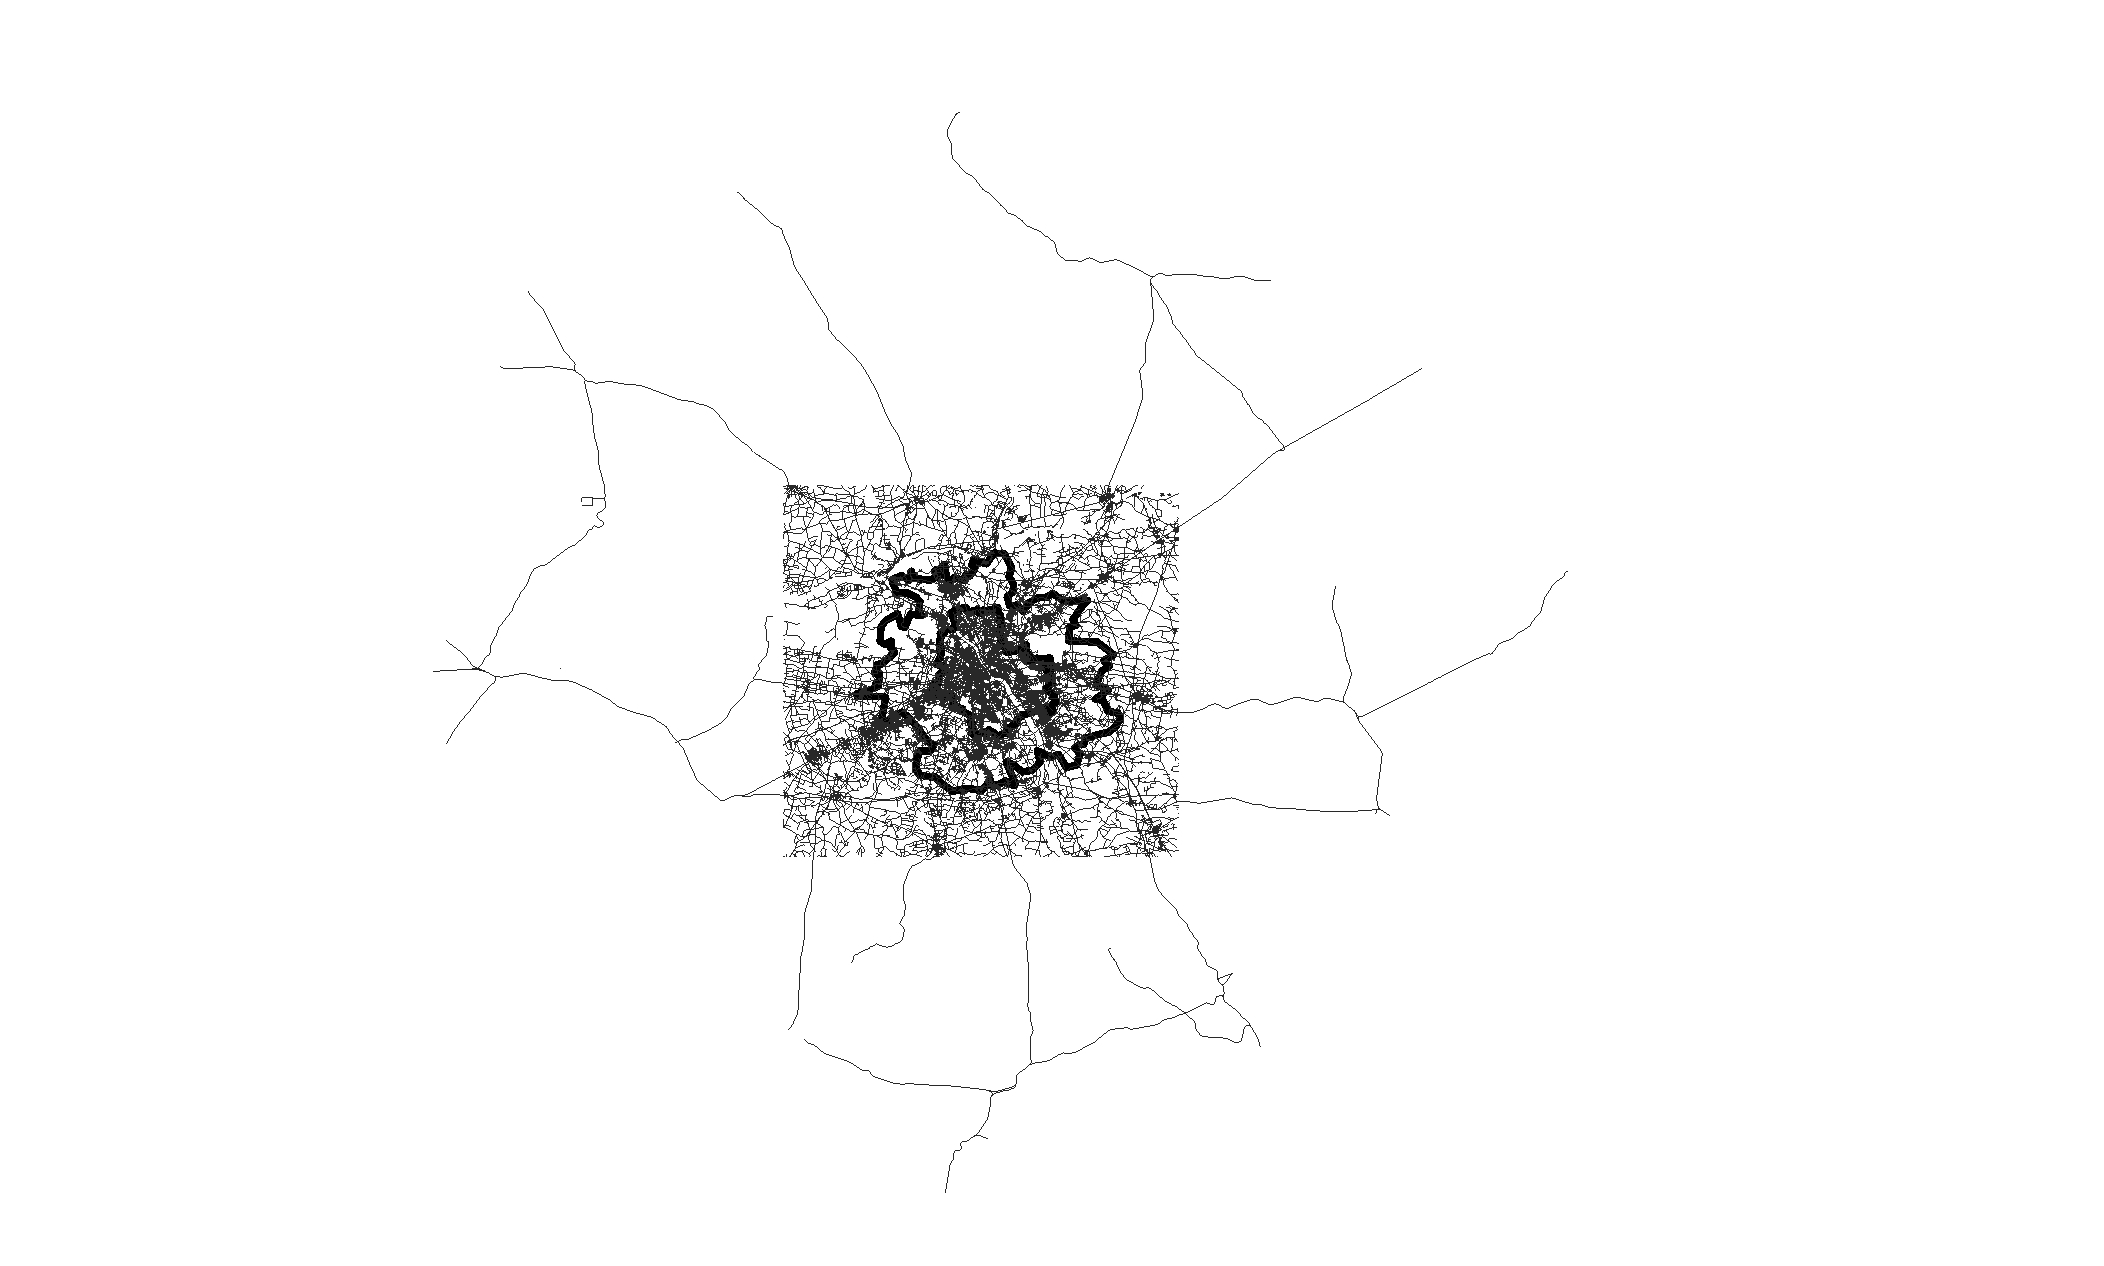
\includegraphics[width=0.9\textwidth]{n1}
 \end{center}  
 \end{figure} 
\end{frame}

\begin{frame}{Obszar}{Zasięg sieci - wycinek OSM}
\begin{figure}
\begin{center}
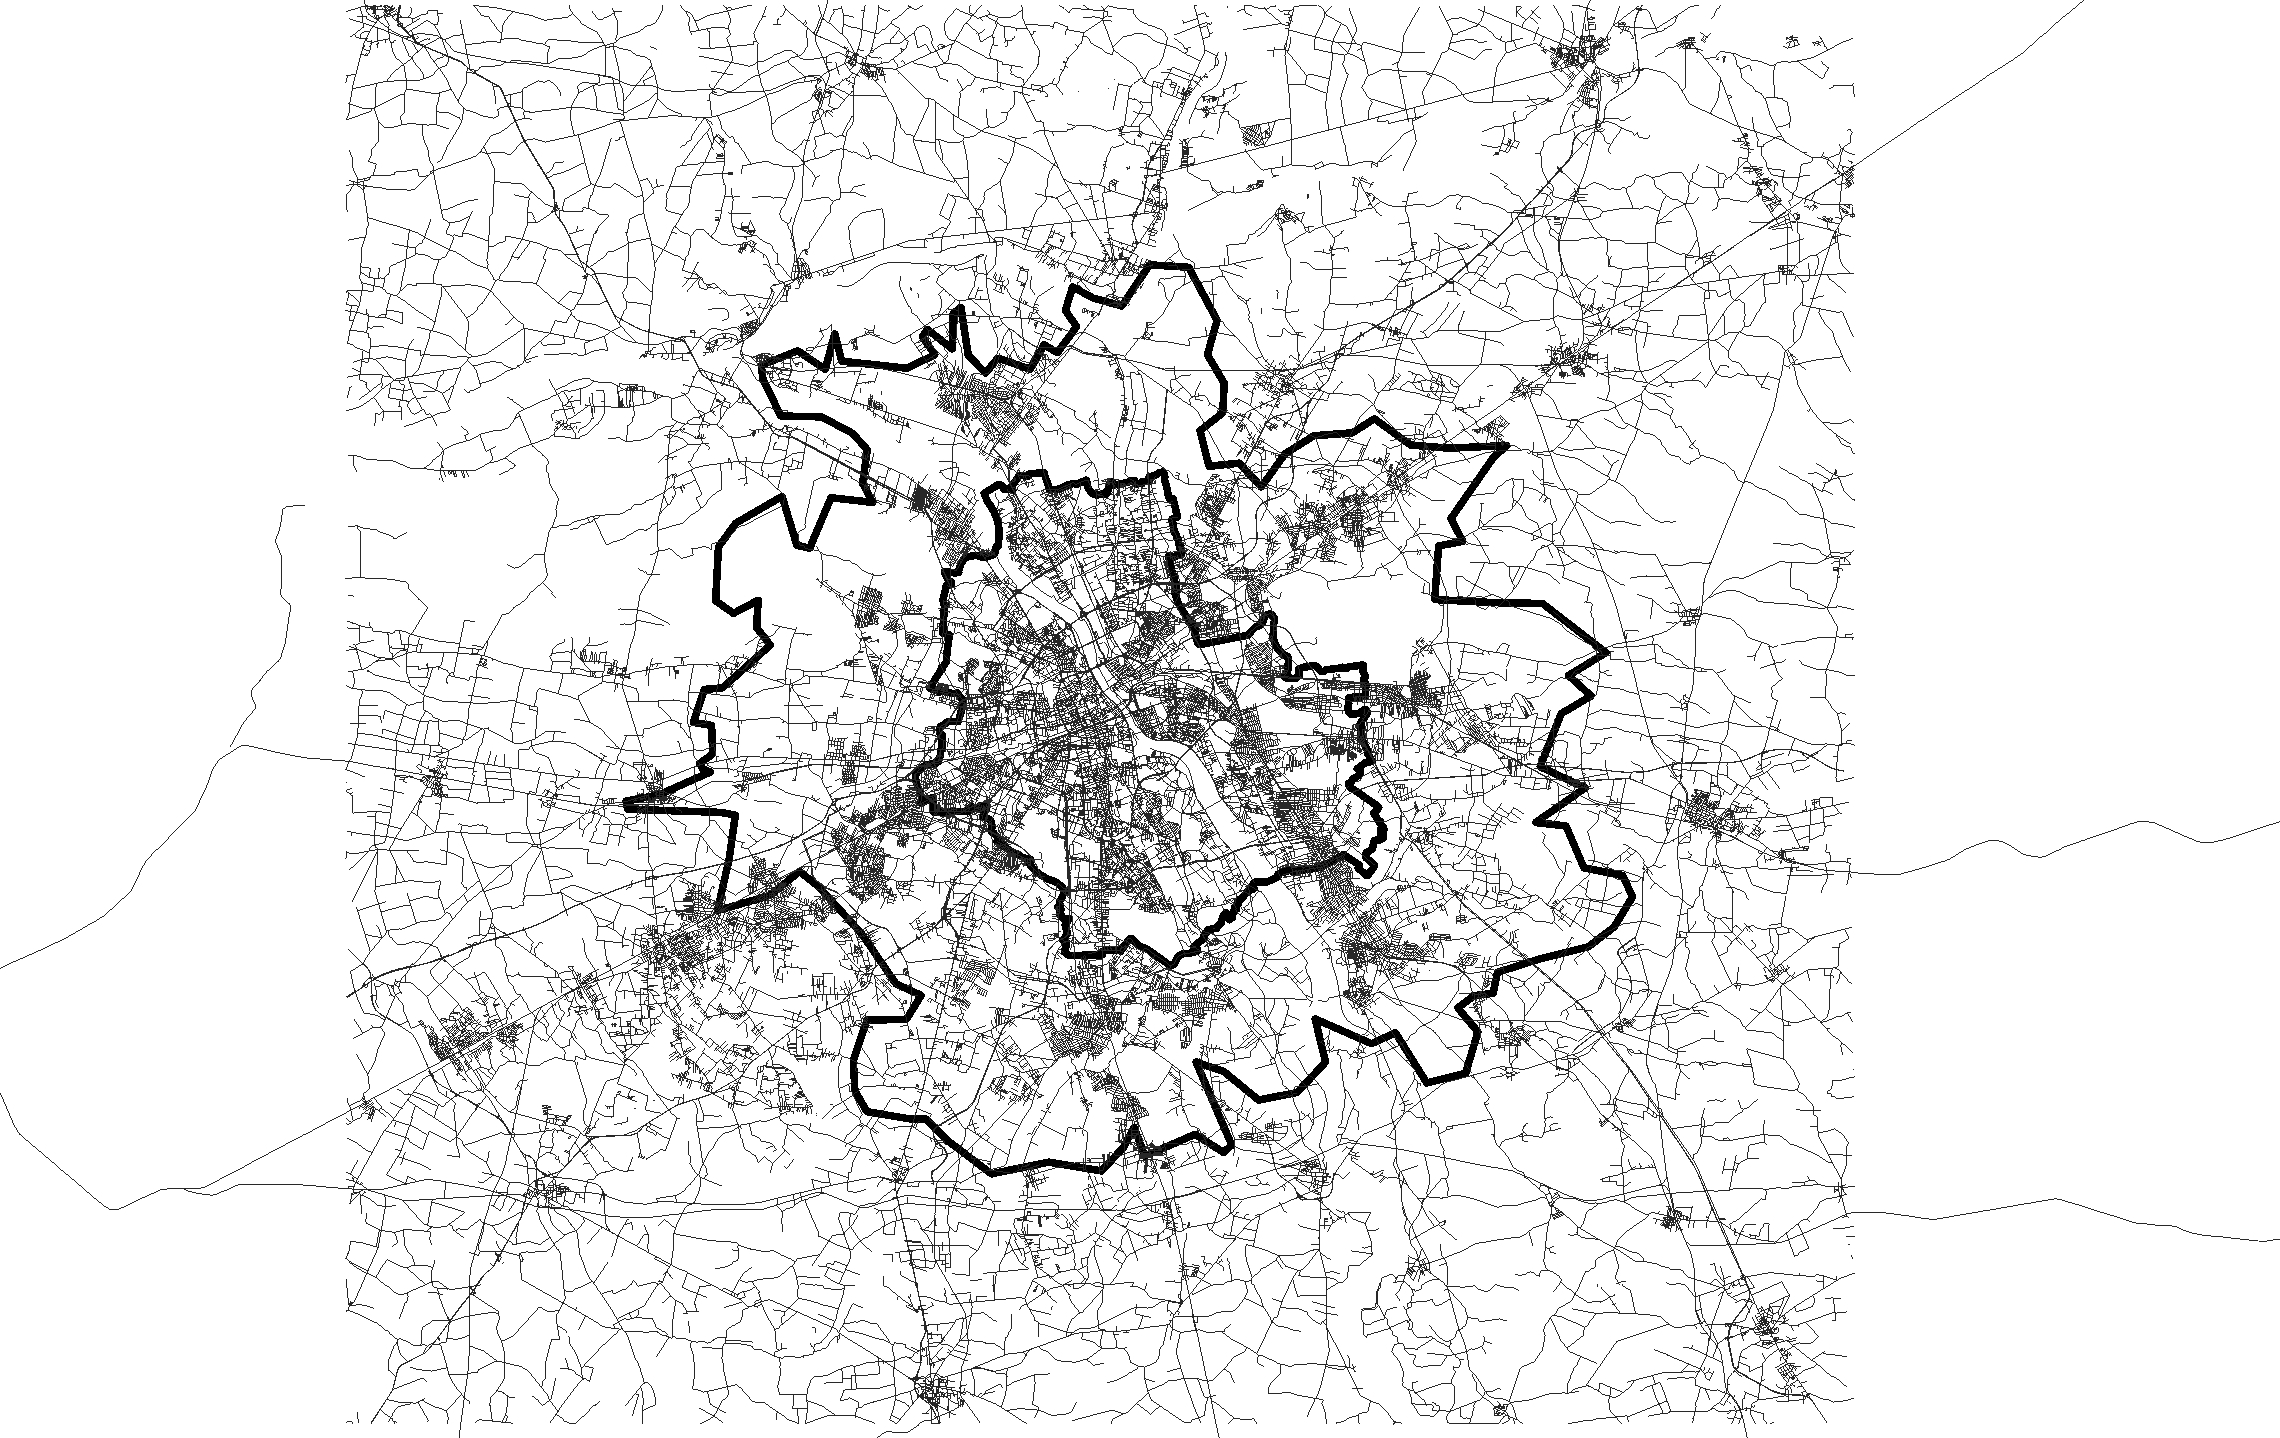
\includegraphics[width=0.9\textwidth]{n2}
 \end{center}
 \end{figure} 
\end{frame}

\begin{frame}{Obszar}{Aglomeracja Warszawska}
\begin{figure}
\begin{center}
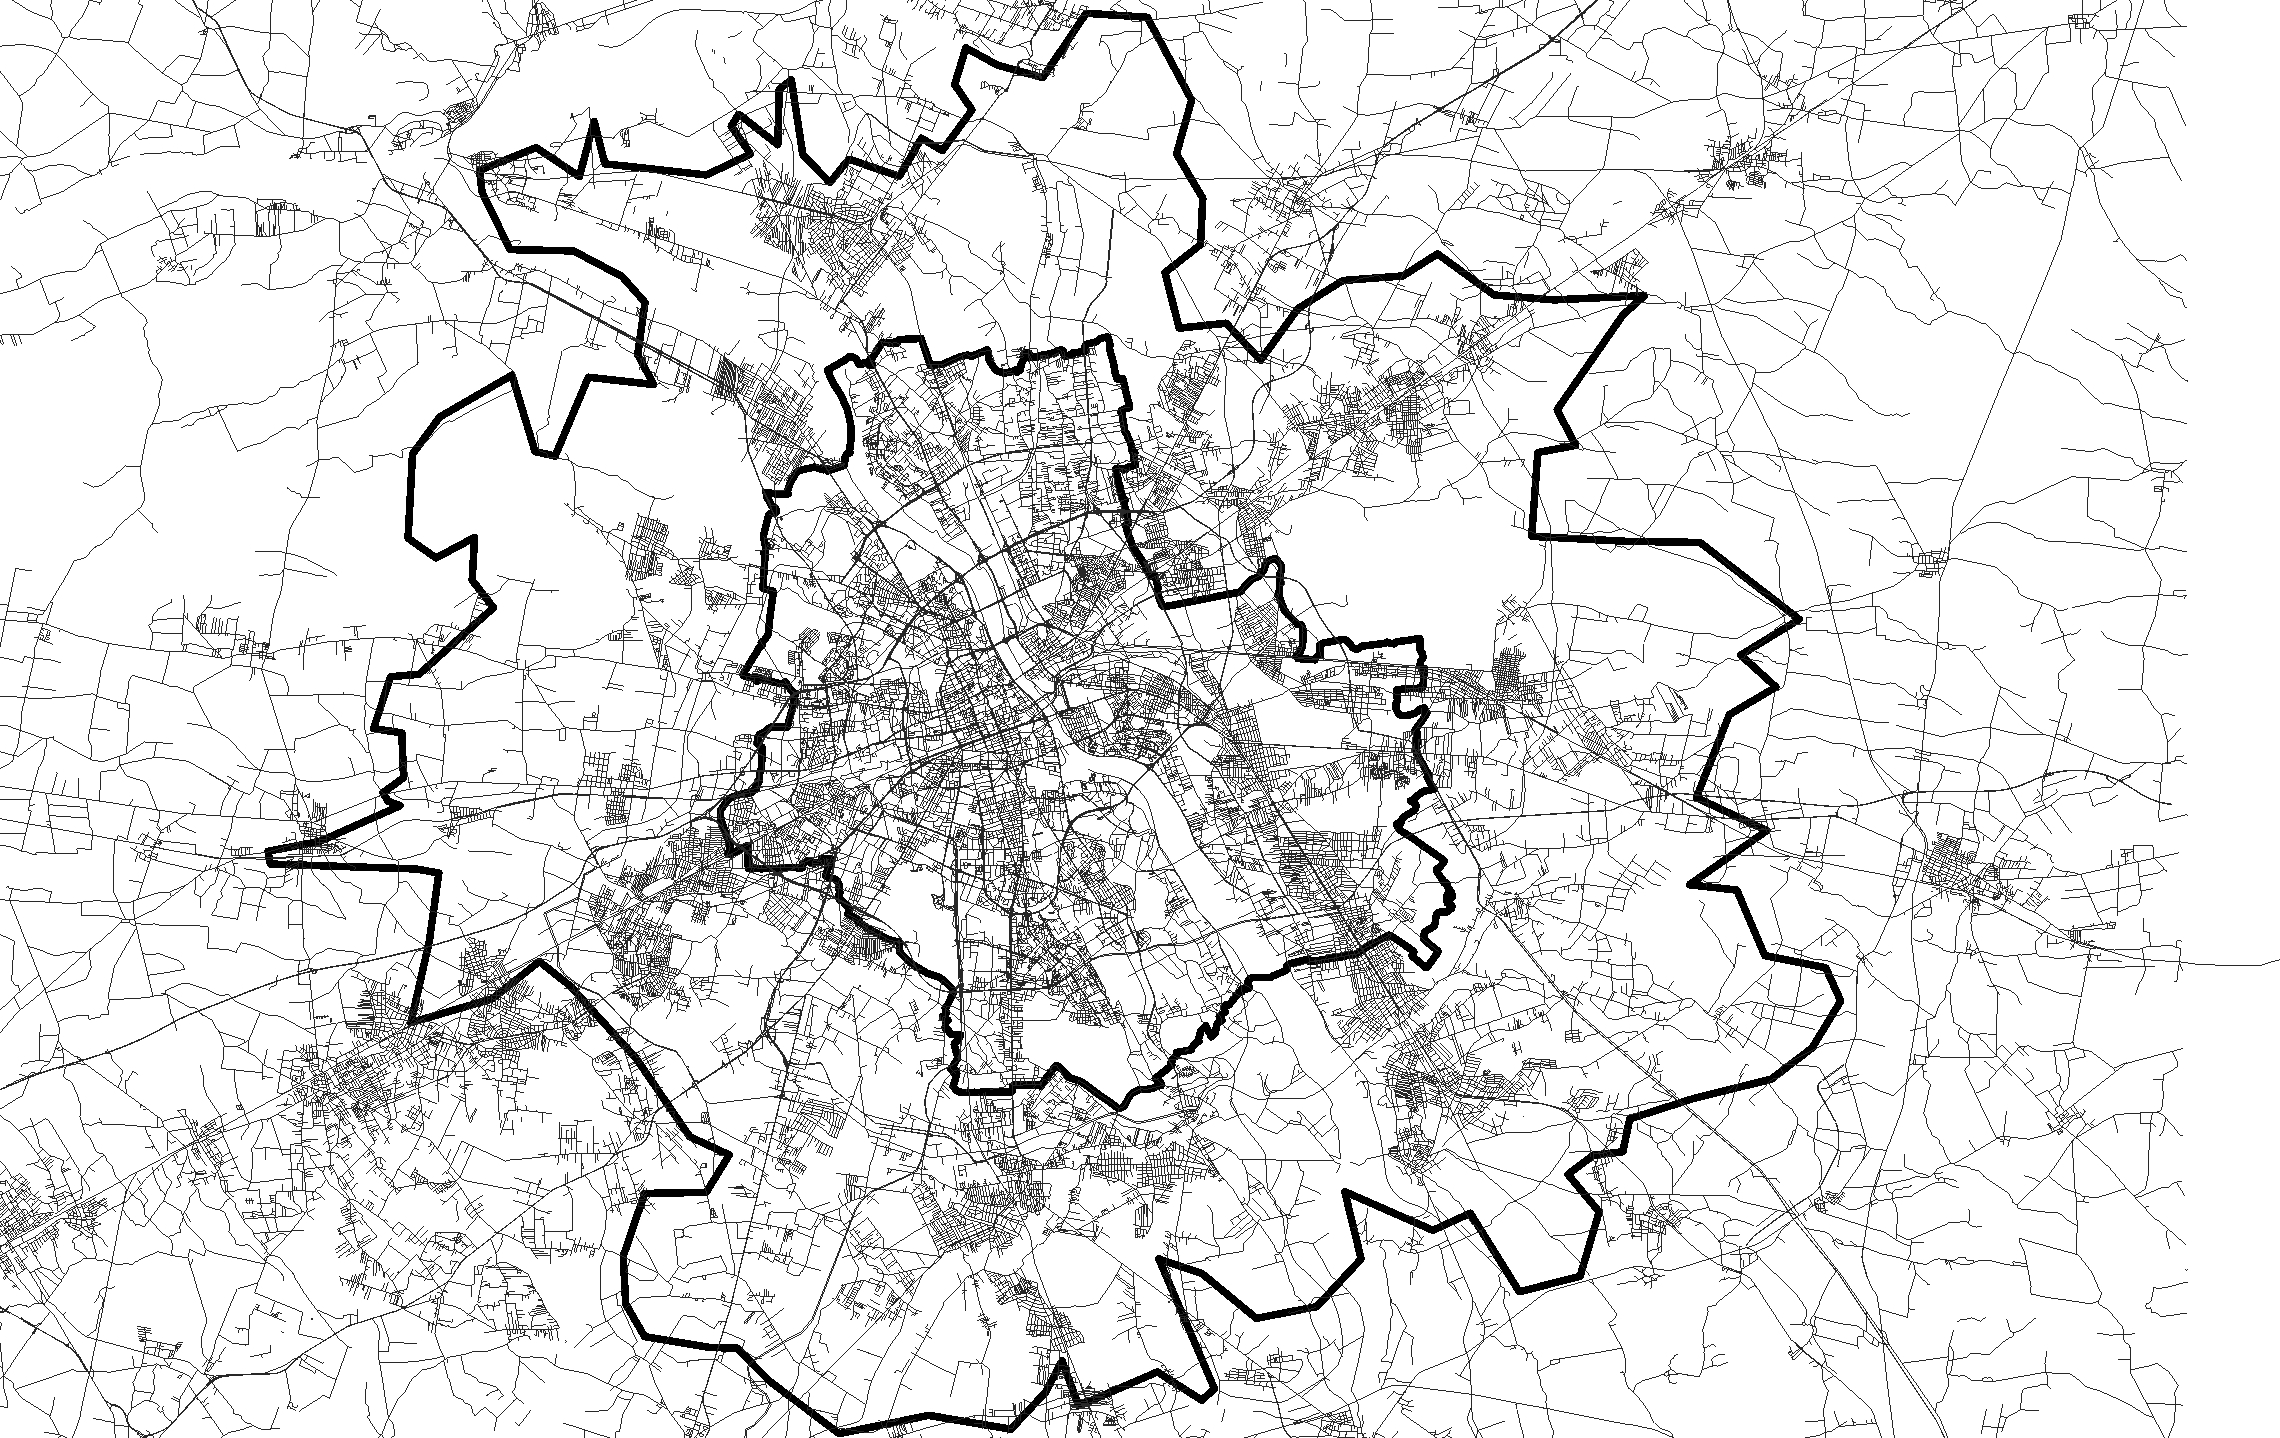
\includegraphics[width=0.9\textwidth]{n3}
 \end{center} 
 \end{figure} 
\end{frame}

\begin{frame}{Obszar}{Warszawa}
\begin{figure}
\begin{center}
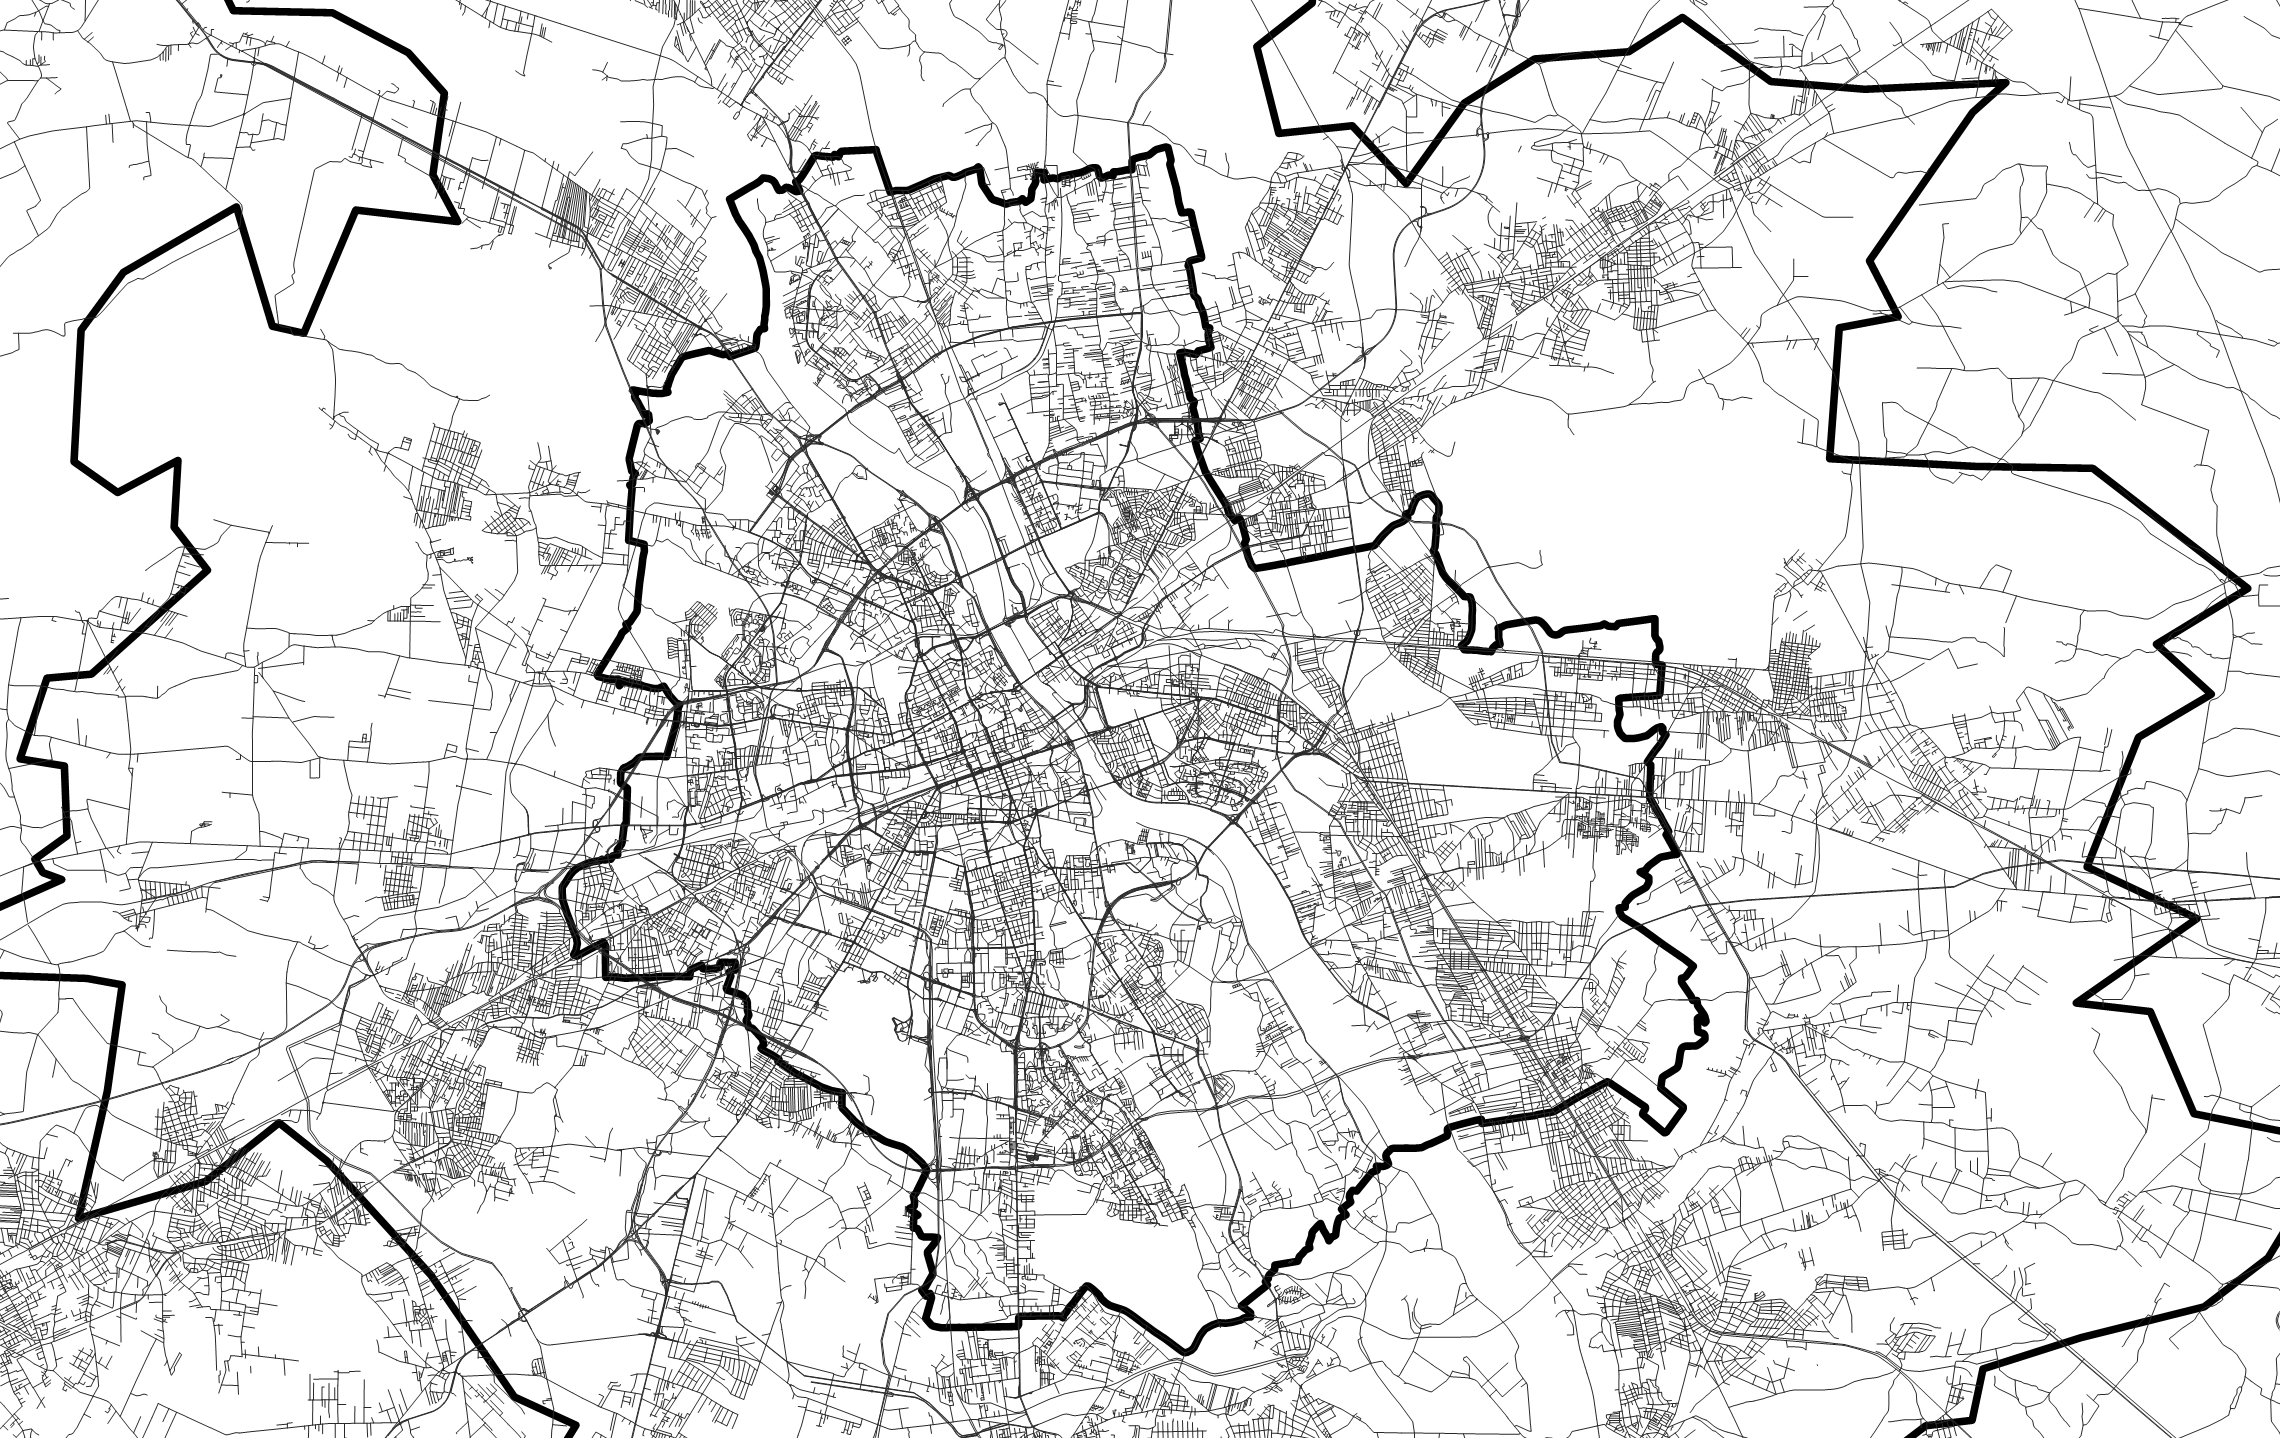
\includegraphics[width=0.9\textwidth]{n4}
 \end{center} 
 \end{figure} 
\end{frame}

\begin{frame}{Obszar}{Śródmieście}
\begin{figure}
\begin{center}
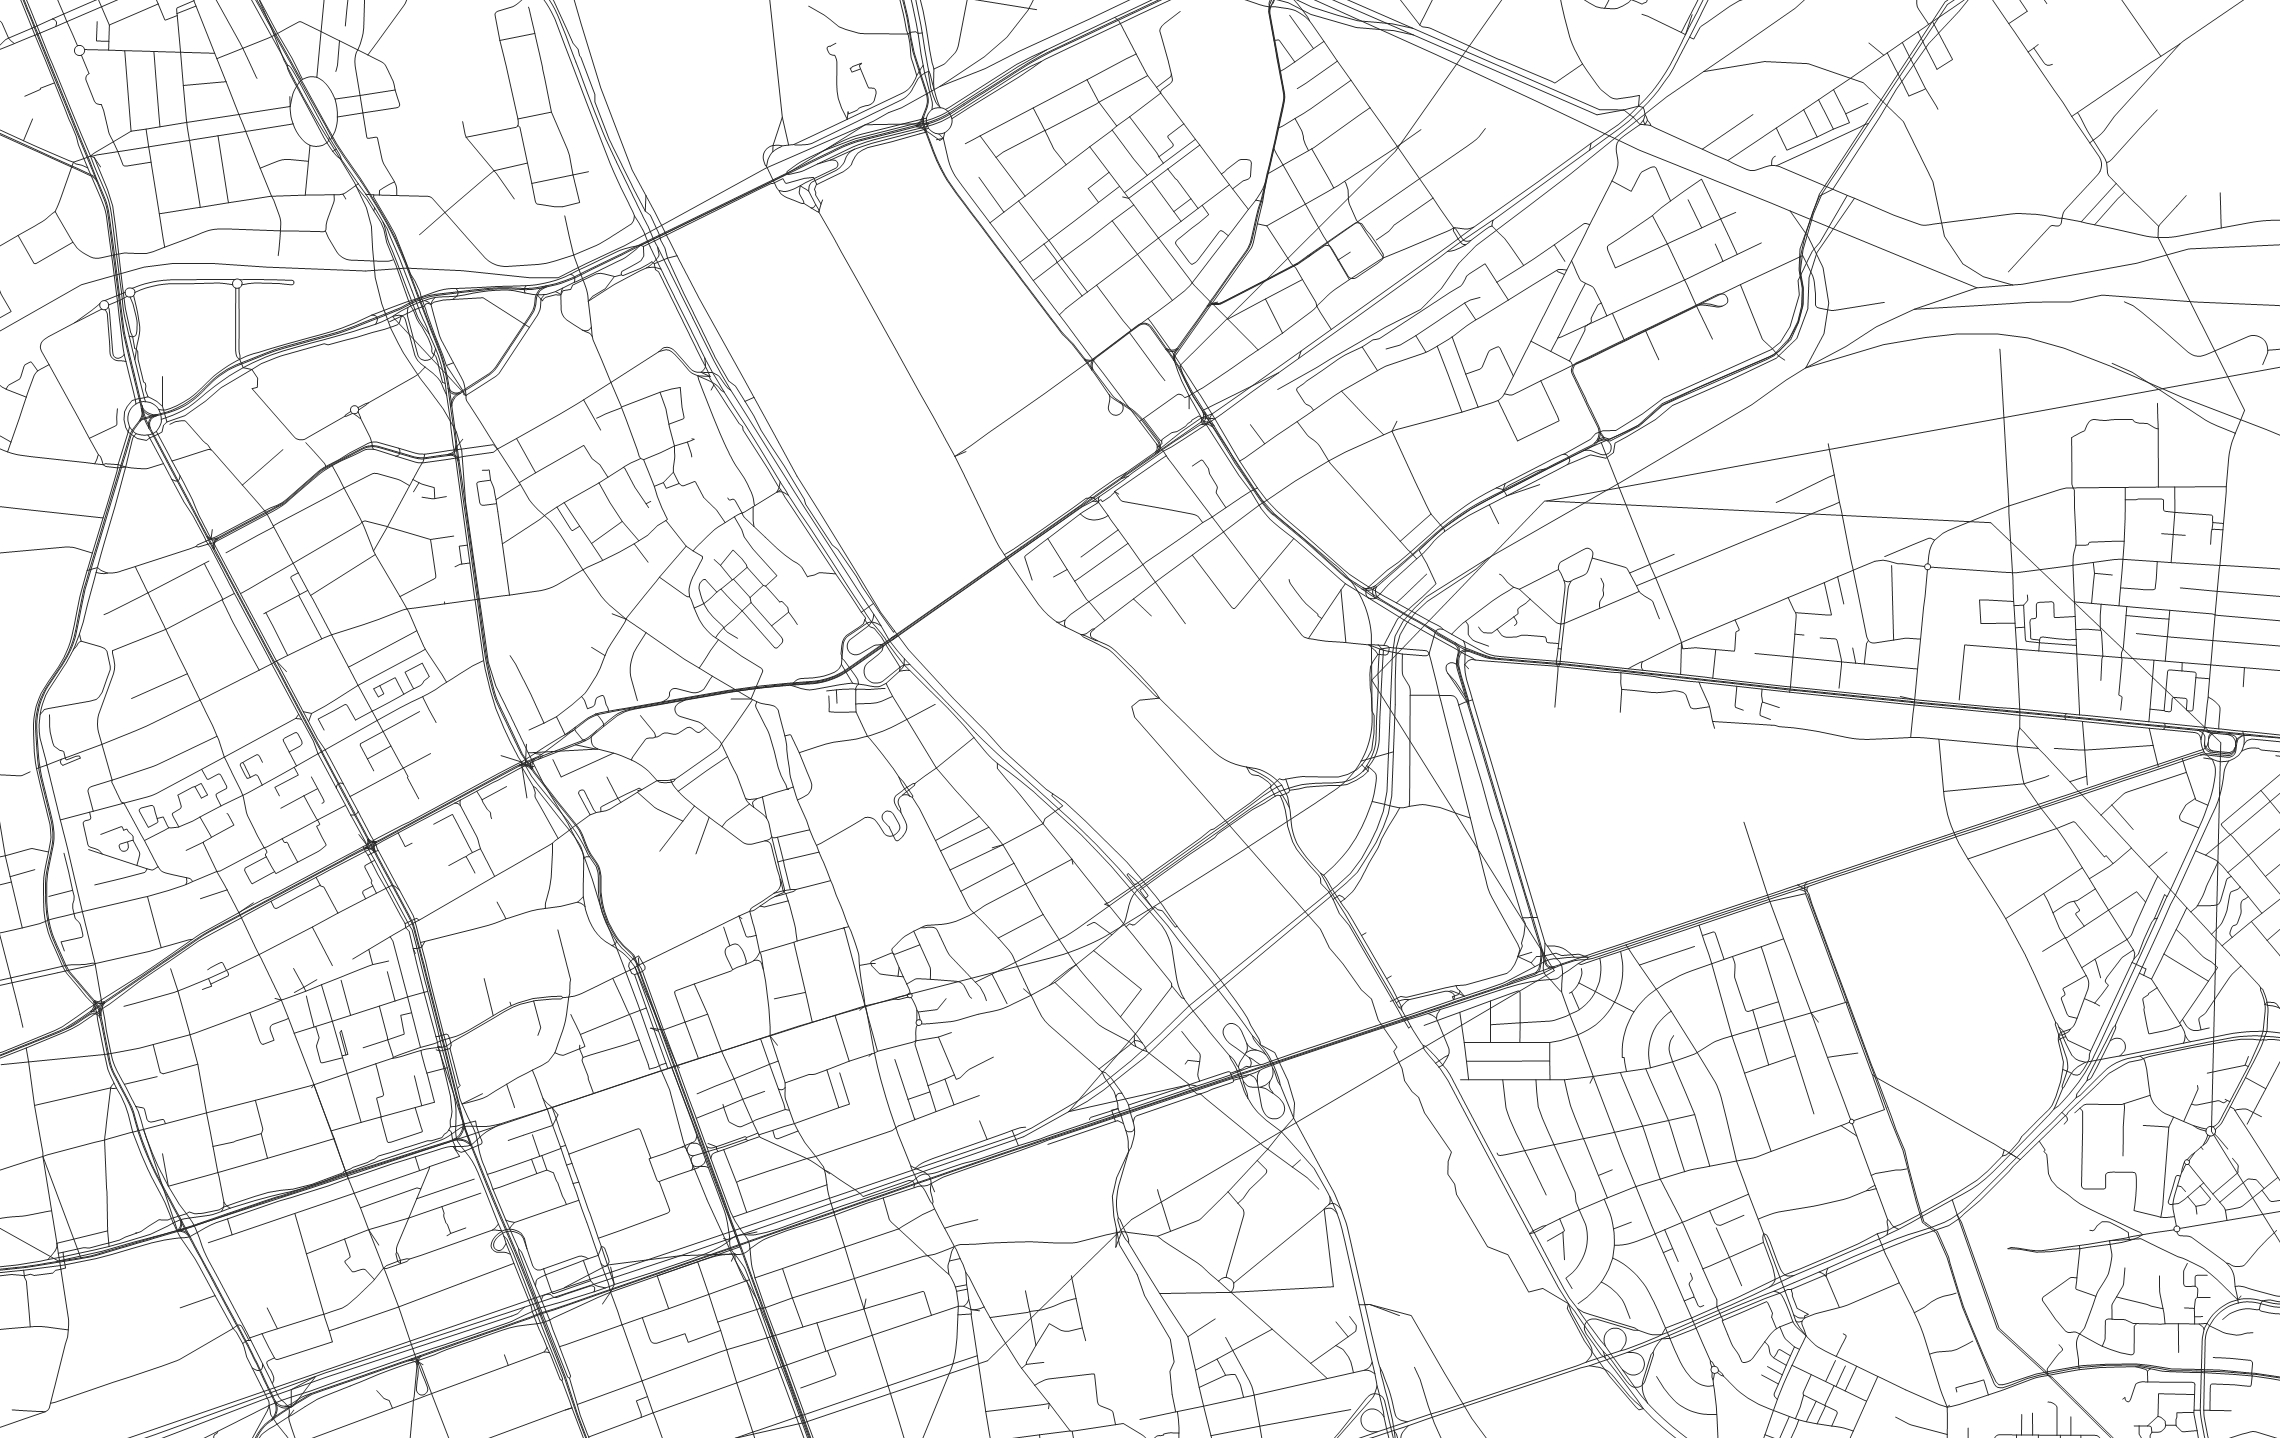
\includegraphics[width=0.9\textwidth]{n5}
 \end{center}
  \end{figure} 
\end{frame}

\subsection{Sieć}
\begin{frame}{Wielkość modelu}{}
\begin{figure}\begin{center}
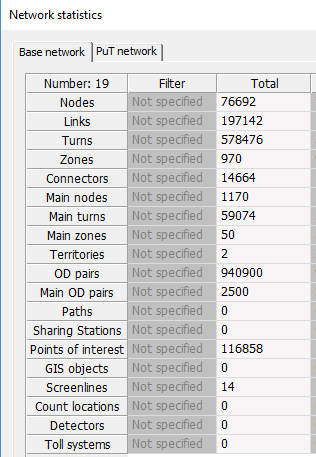
\includegraphics[width=0.4\textwidth]{size}
 \end{center}  \end{figure} 
\end{frame}

\begin{frame}{Węzły}{graf sieci}
\begin{figure}
\begin{center}
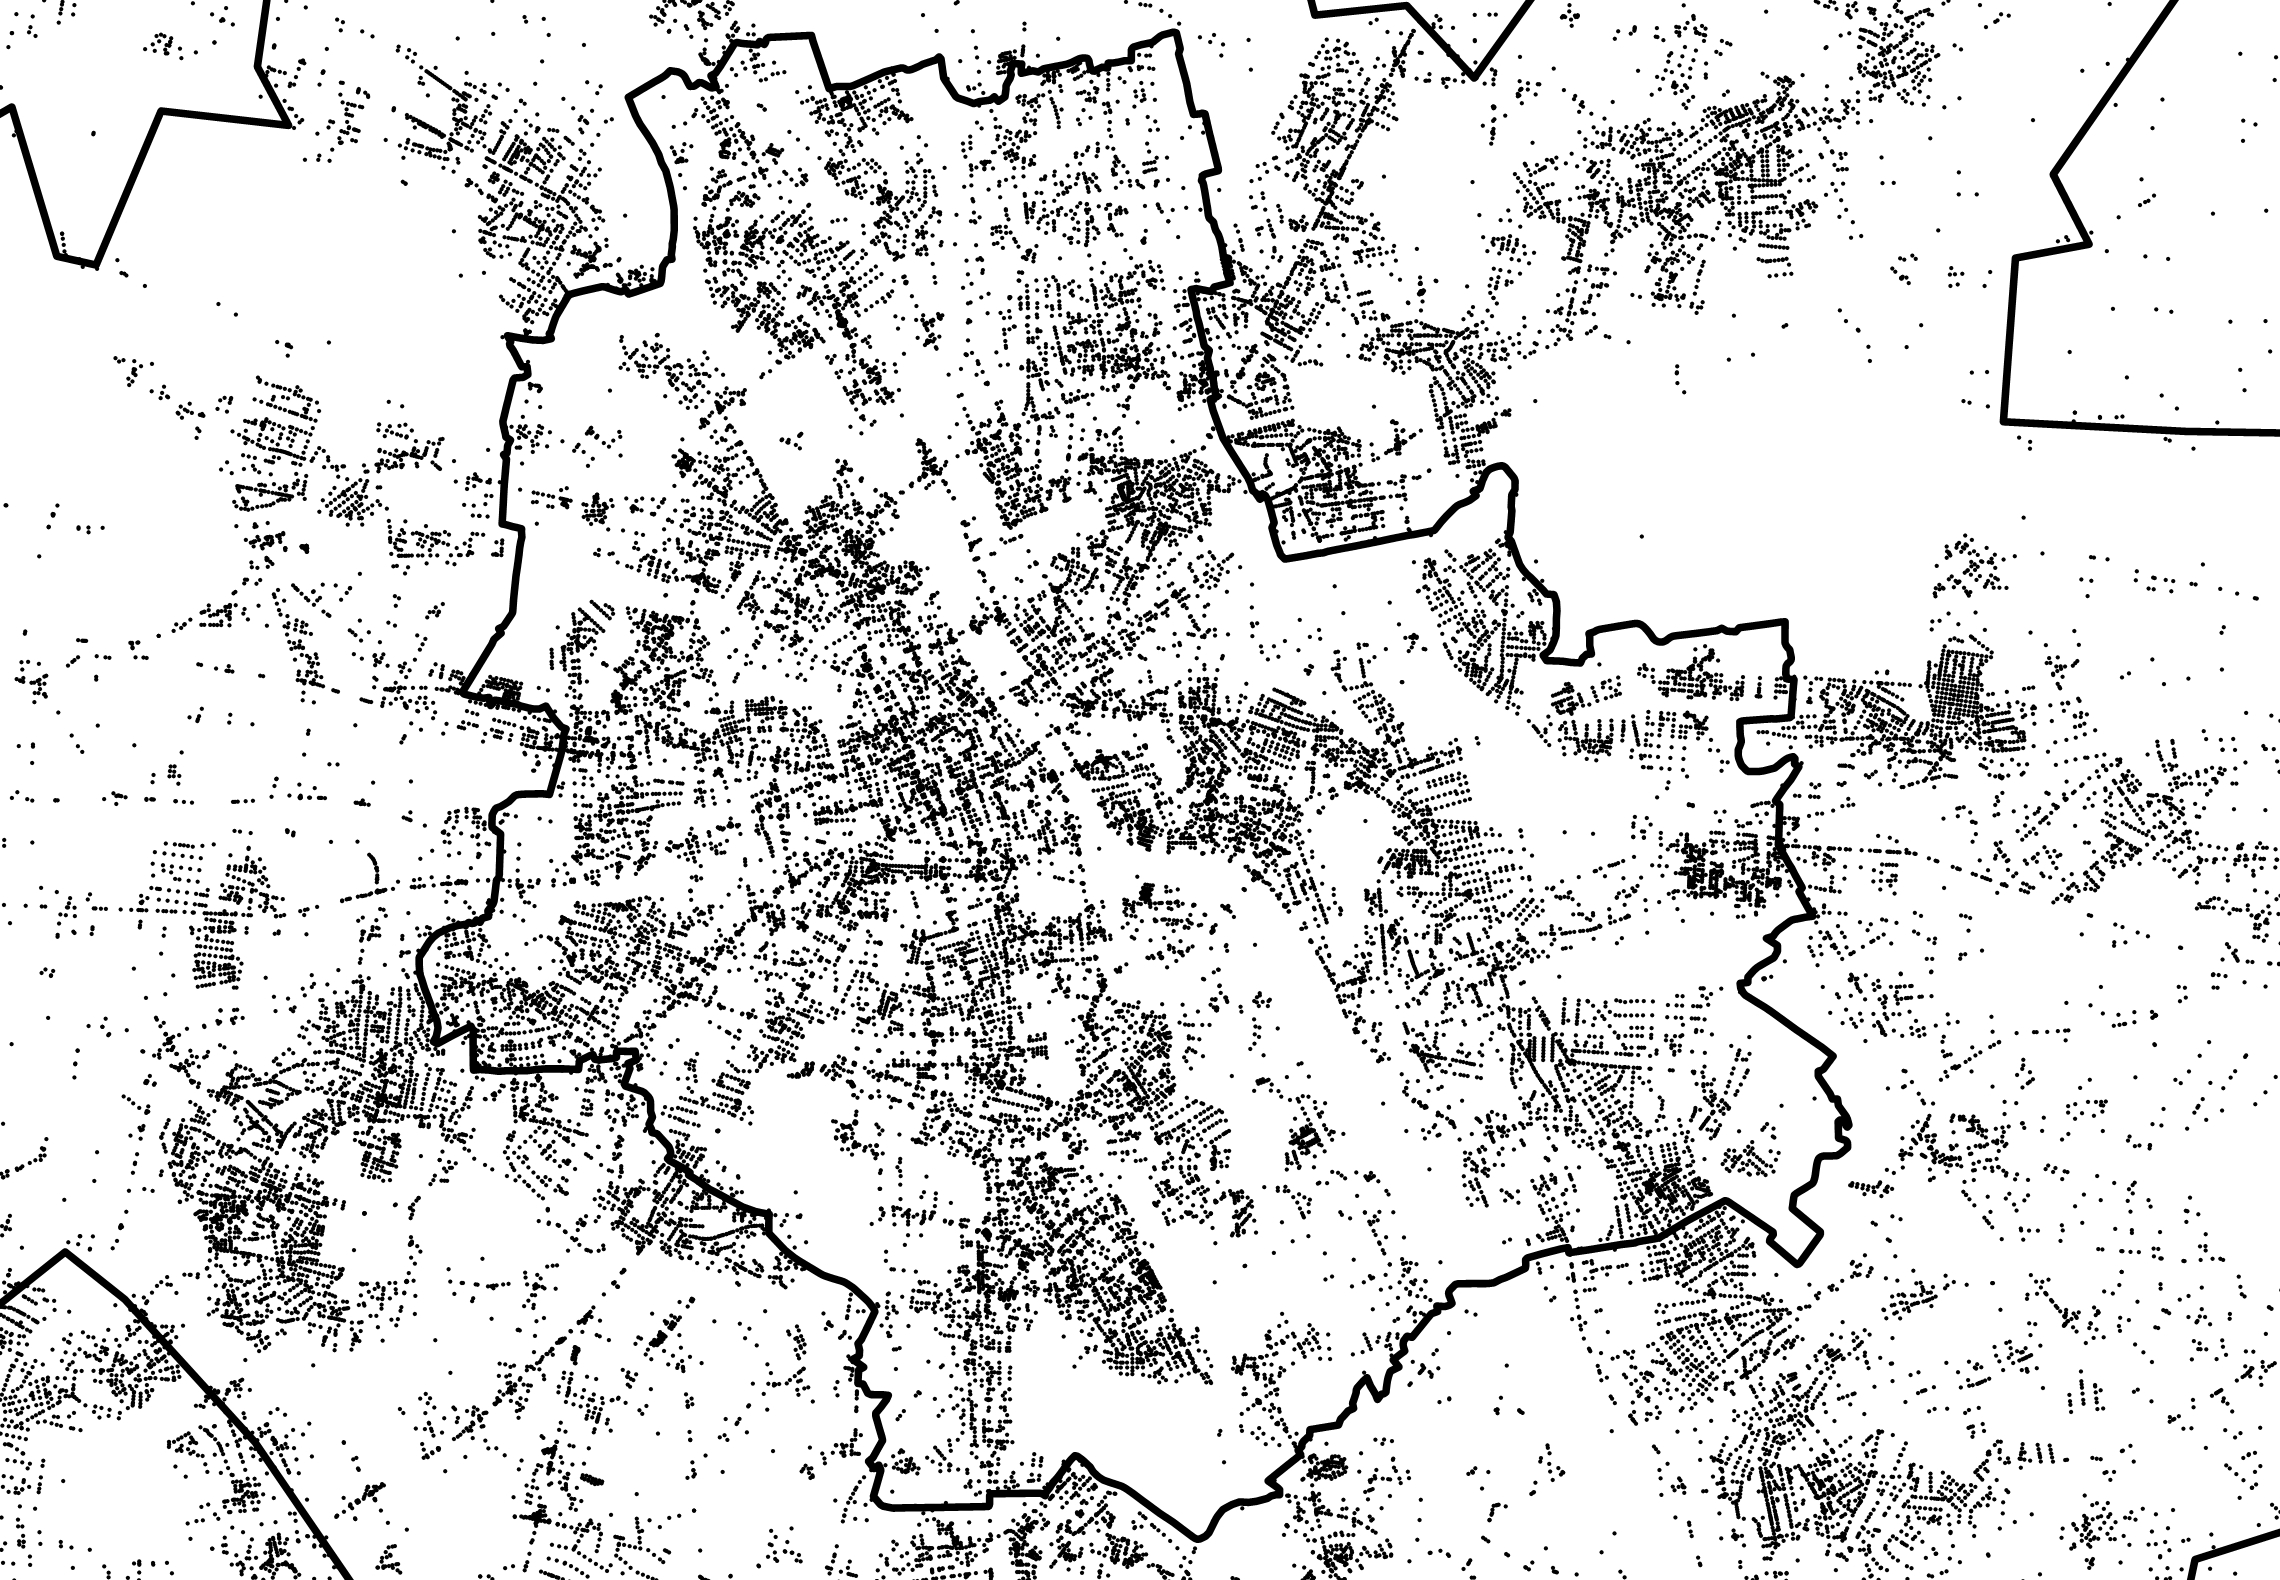
\includegraphics[width=0.9\textwidth]{nodes}
 \end{center}
  \end{figure} 
\end{frame}

\begin{frame}{Odcinki}{kategoryzacja}
\begin{figure}
\begin{center}
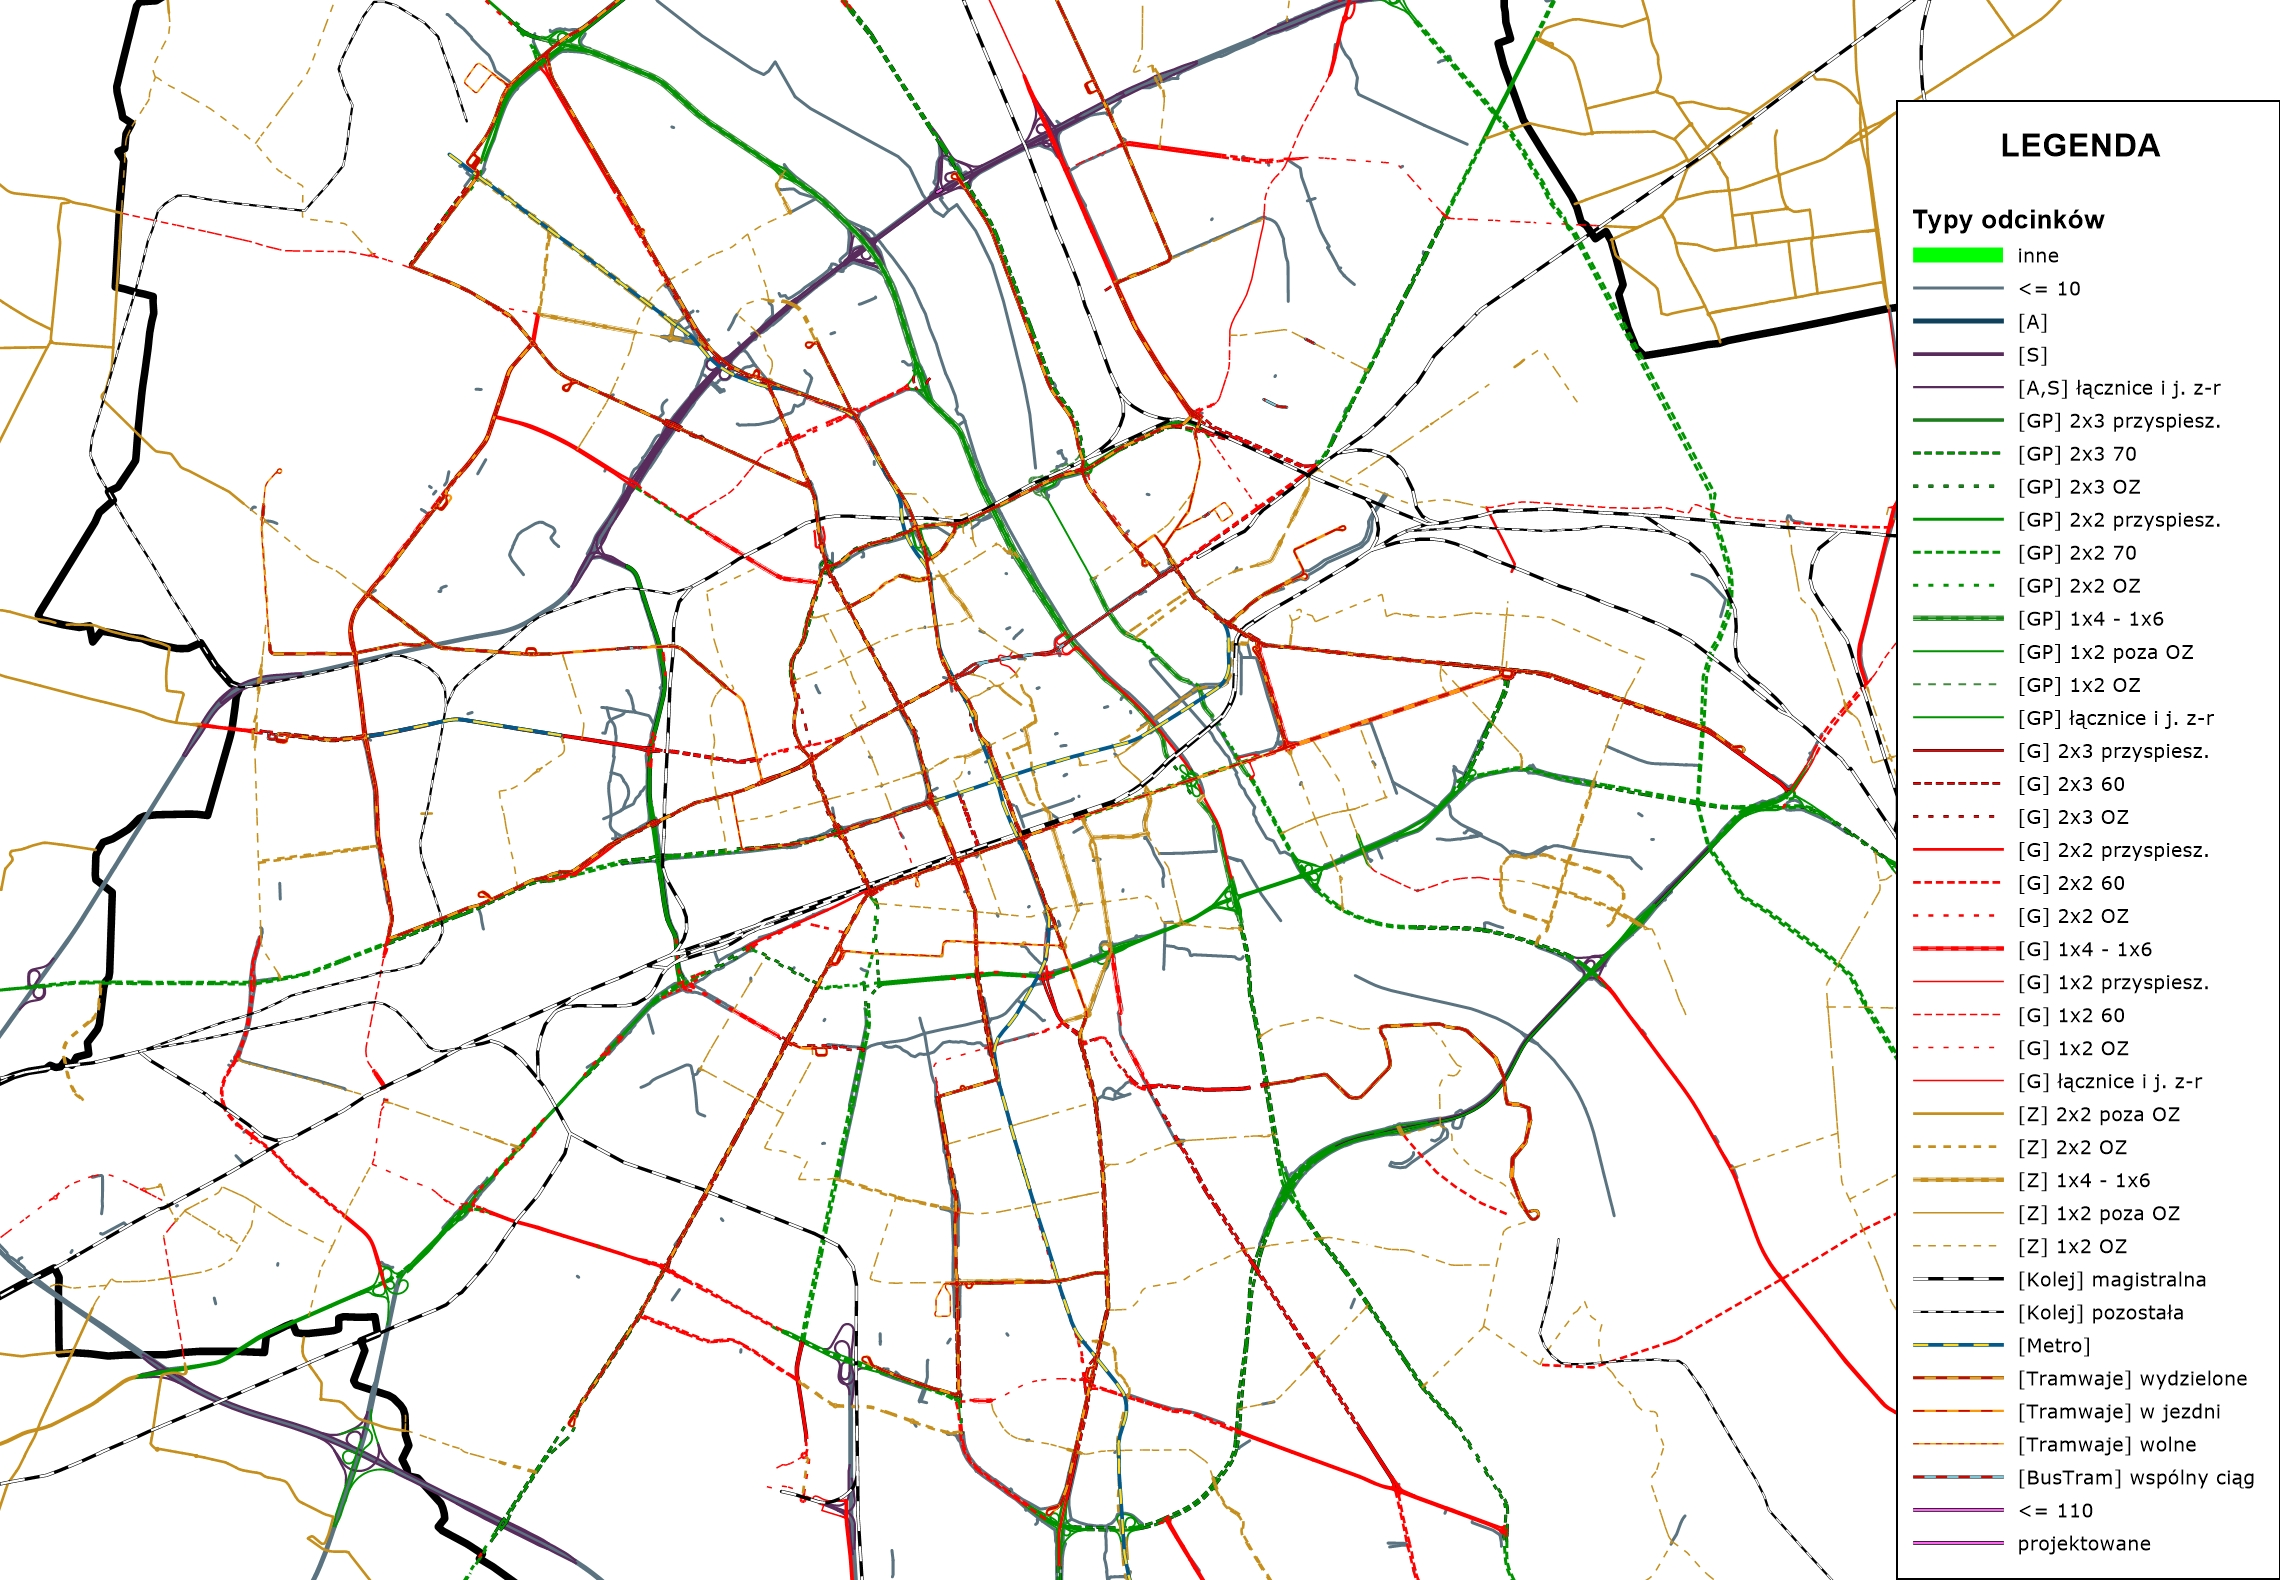
\includegraphics[width=0.9\textwidth]{links}
 \end{center}
  \end{figure} 
\end{frame}

\begin{frame}{Odcinki}{geometria}
\begin{figure}
\begin{center}
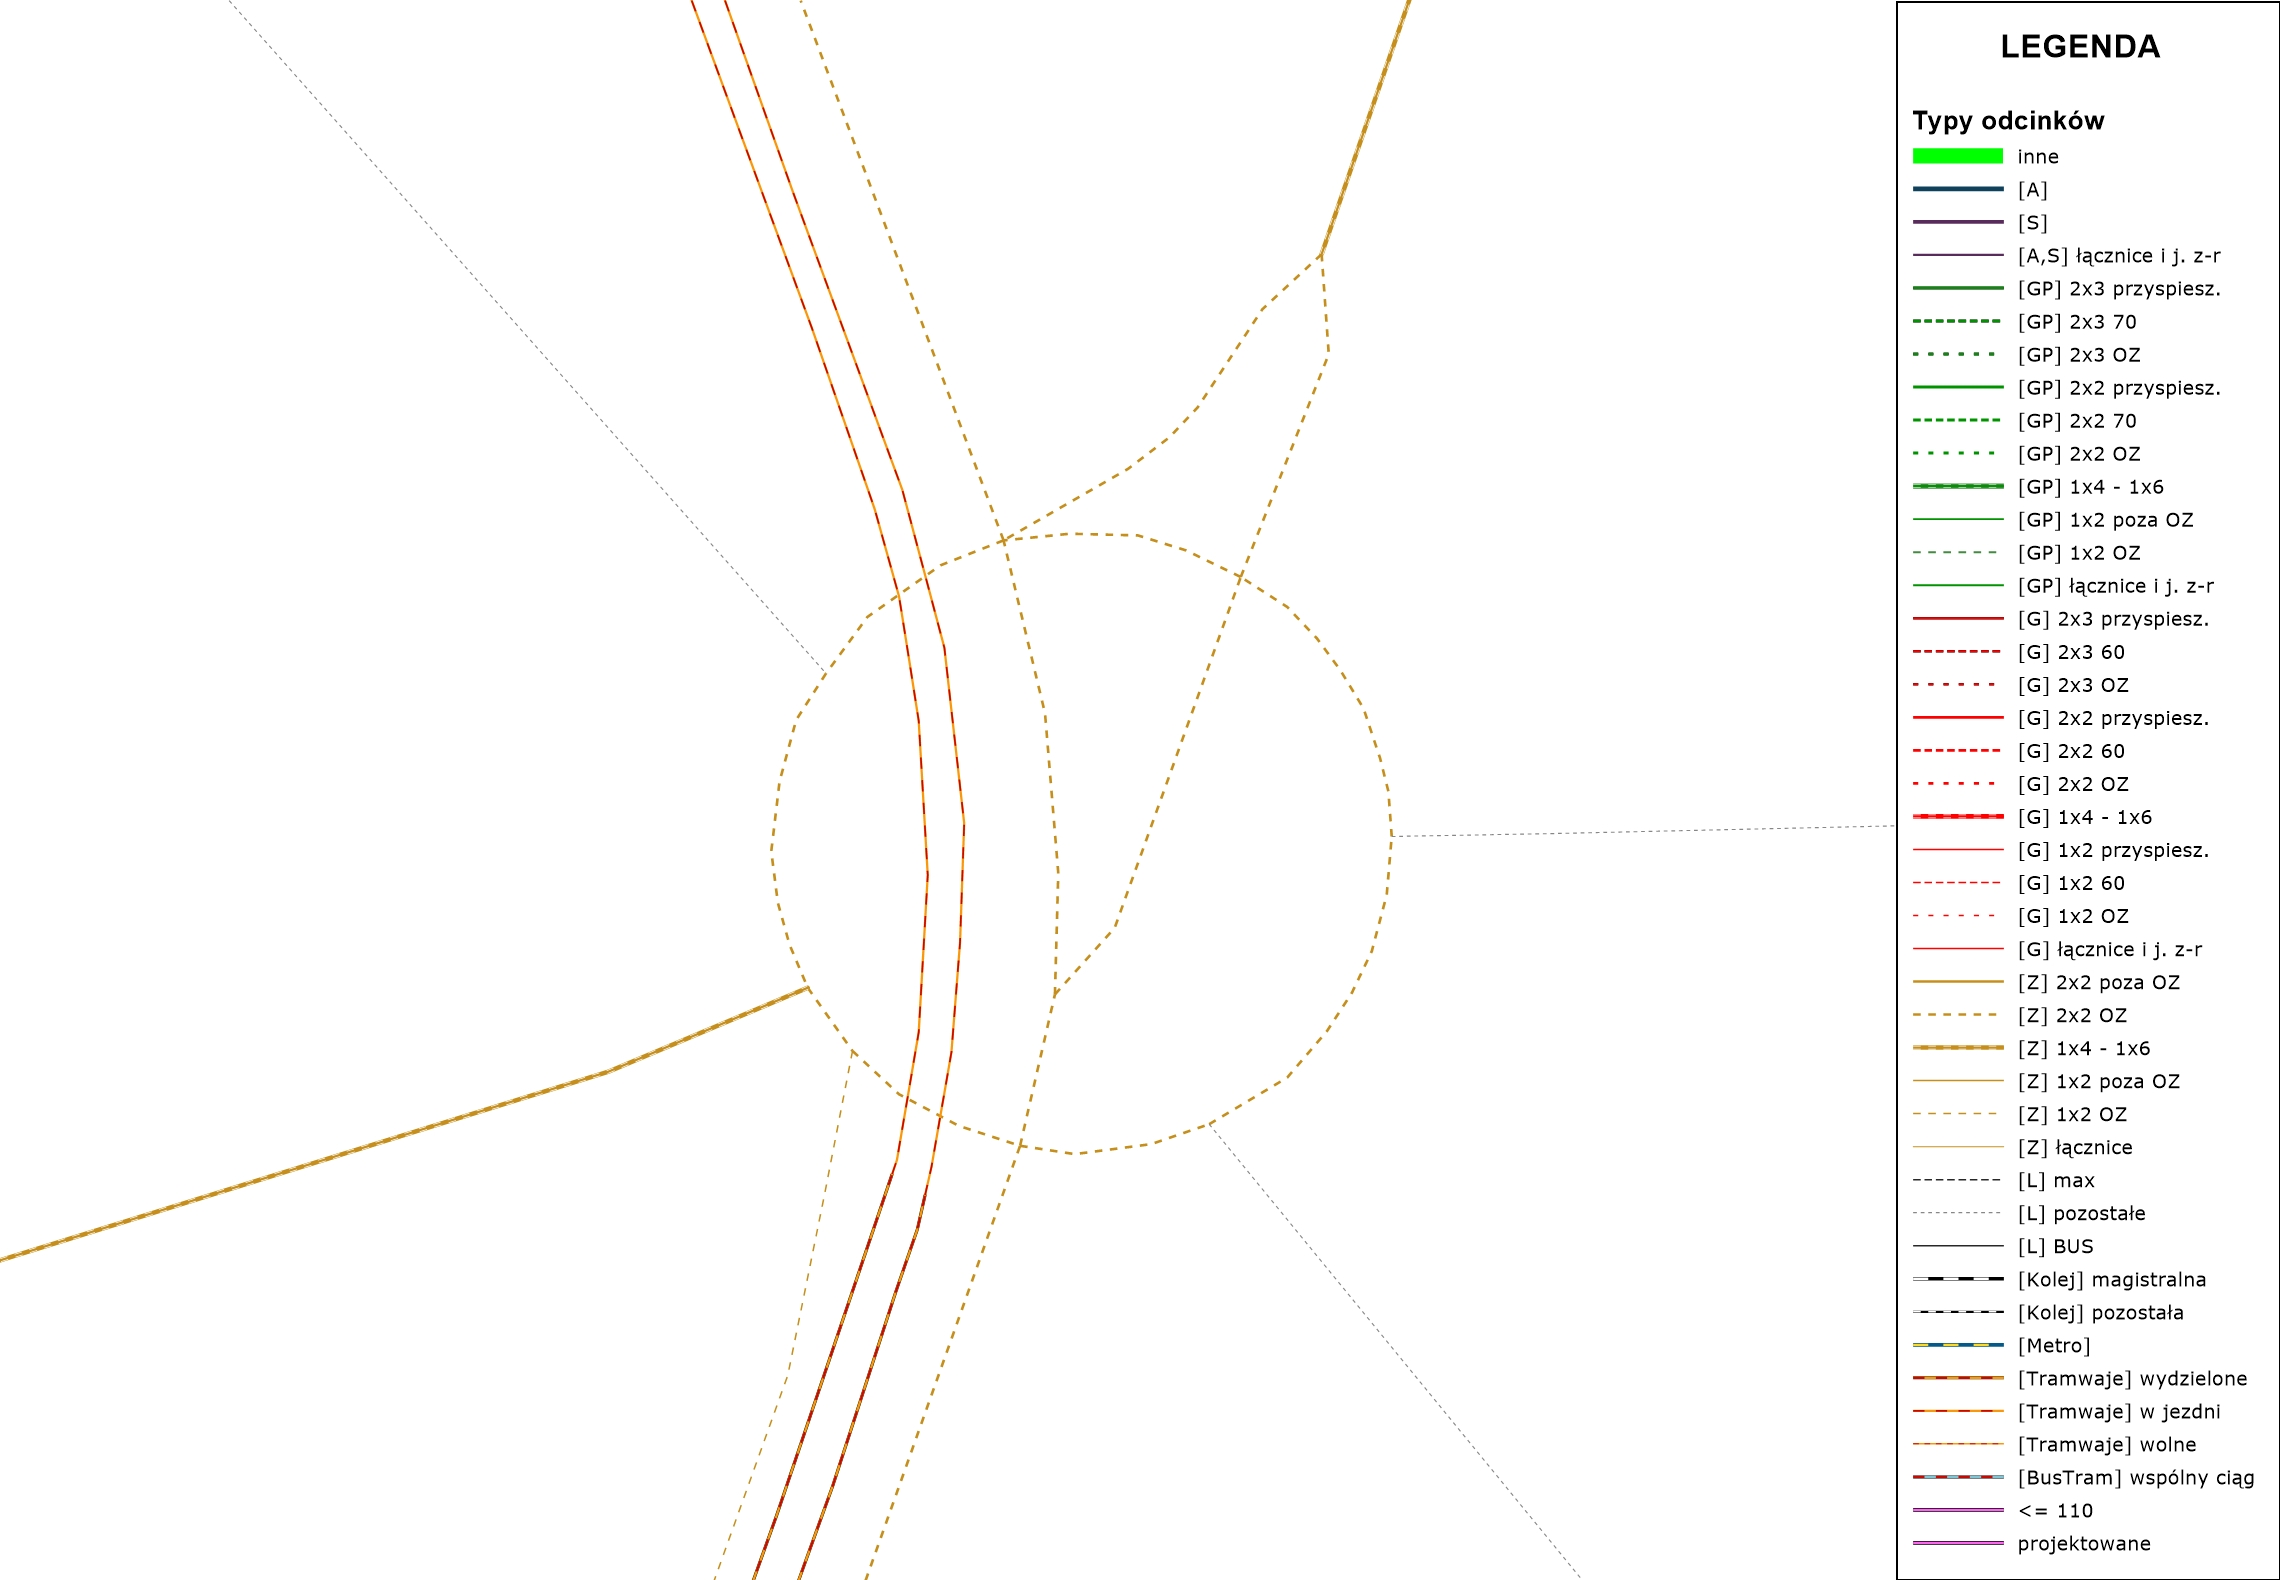
\includegraphics[width=0.9\textwidth]{geom}
 \end{center}
  \end{figure} 
\end{frame}

\begin{frame}{Odcinki}{układ lokalny}
\begin{figure}
\begin{center}
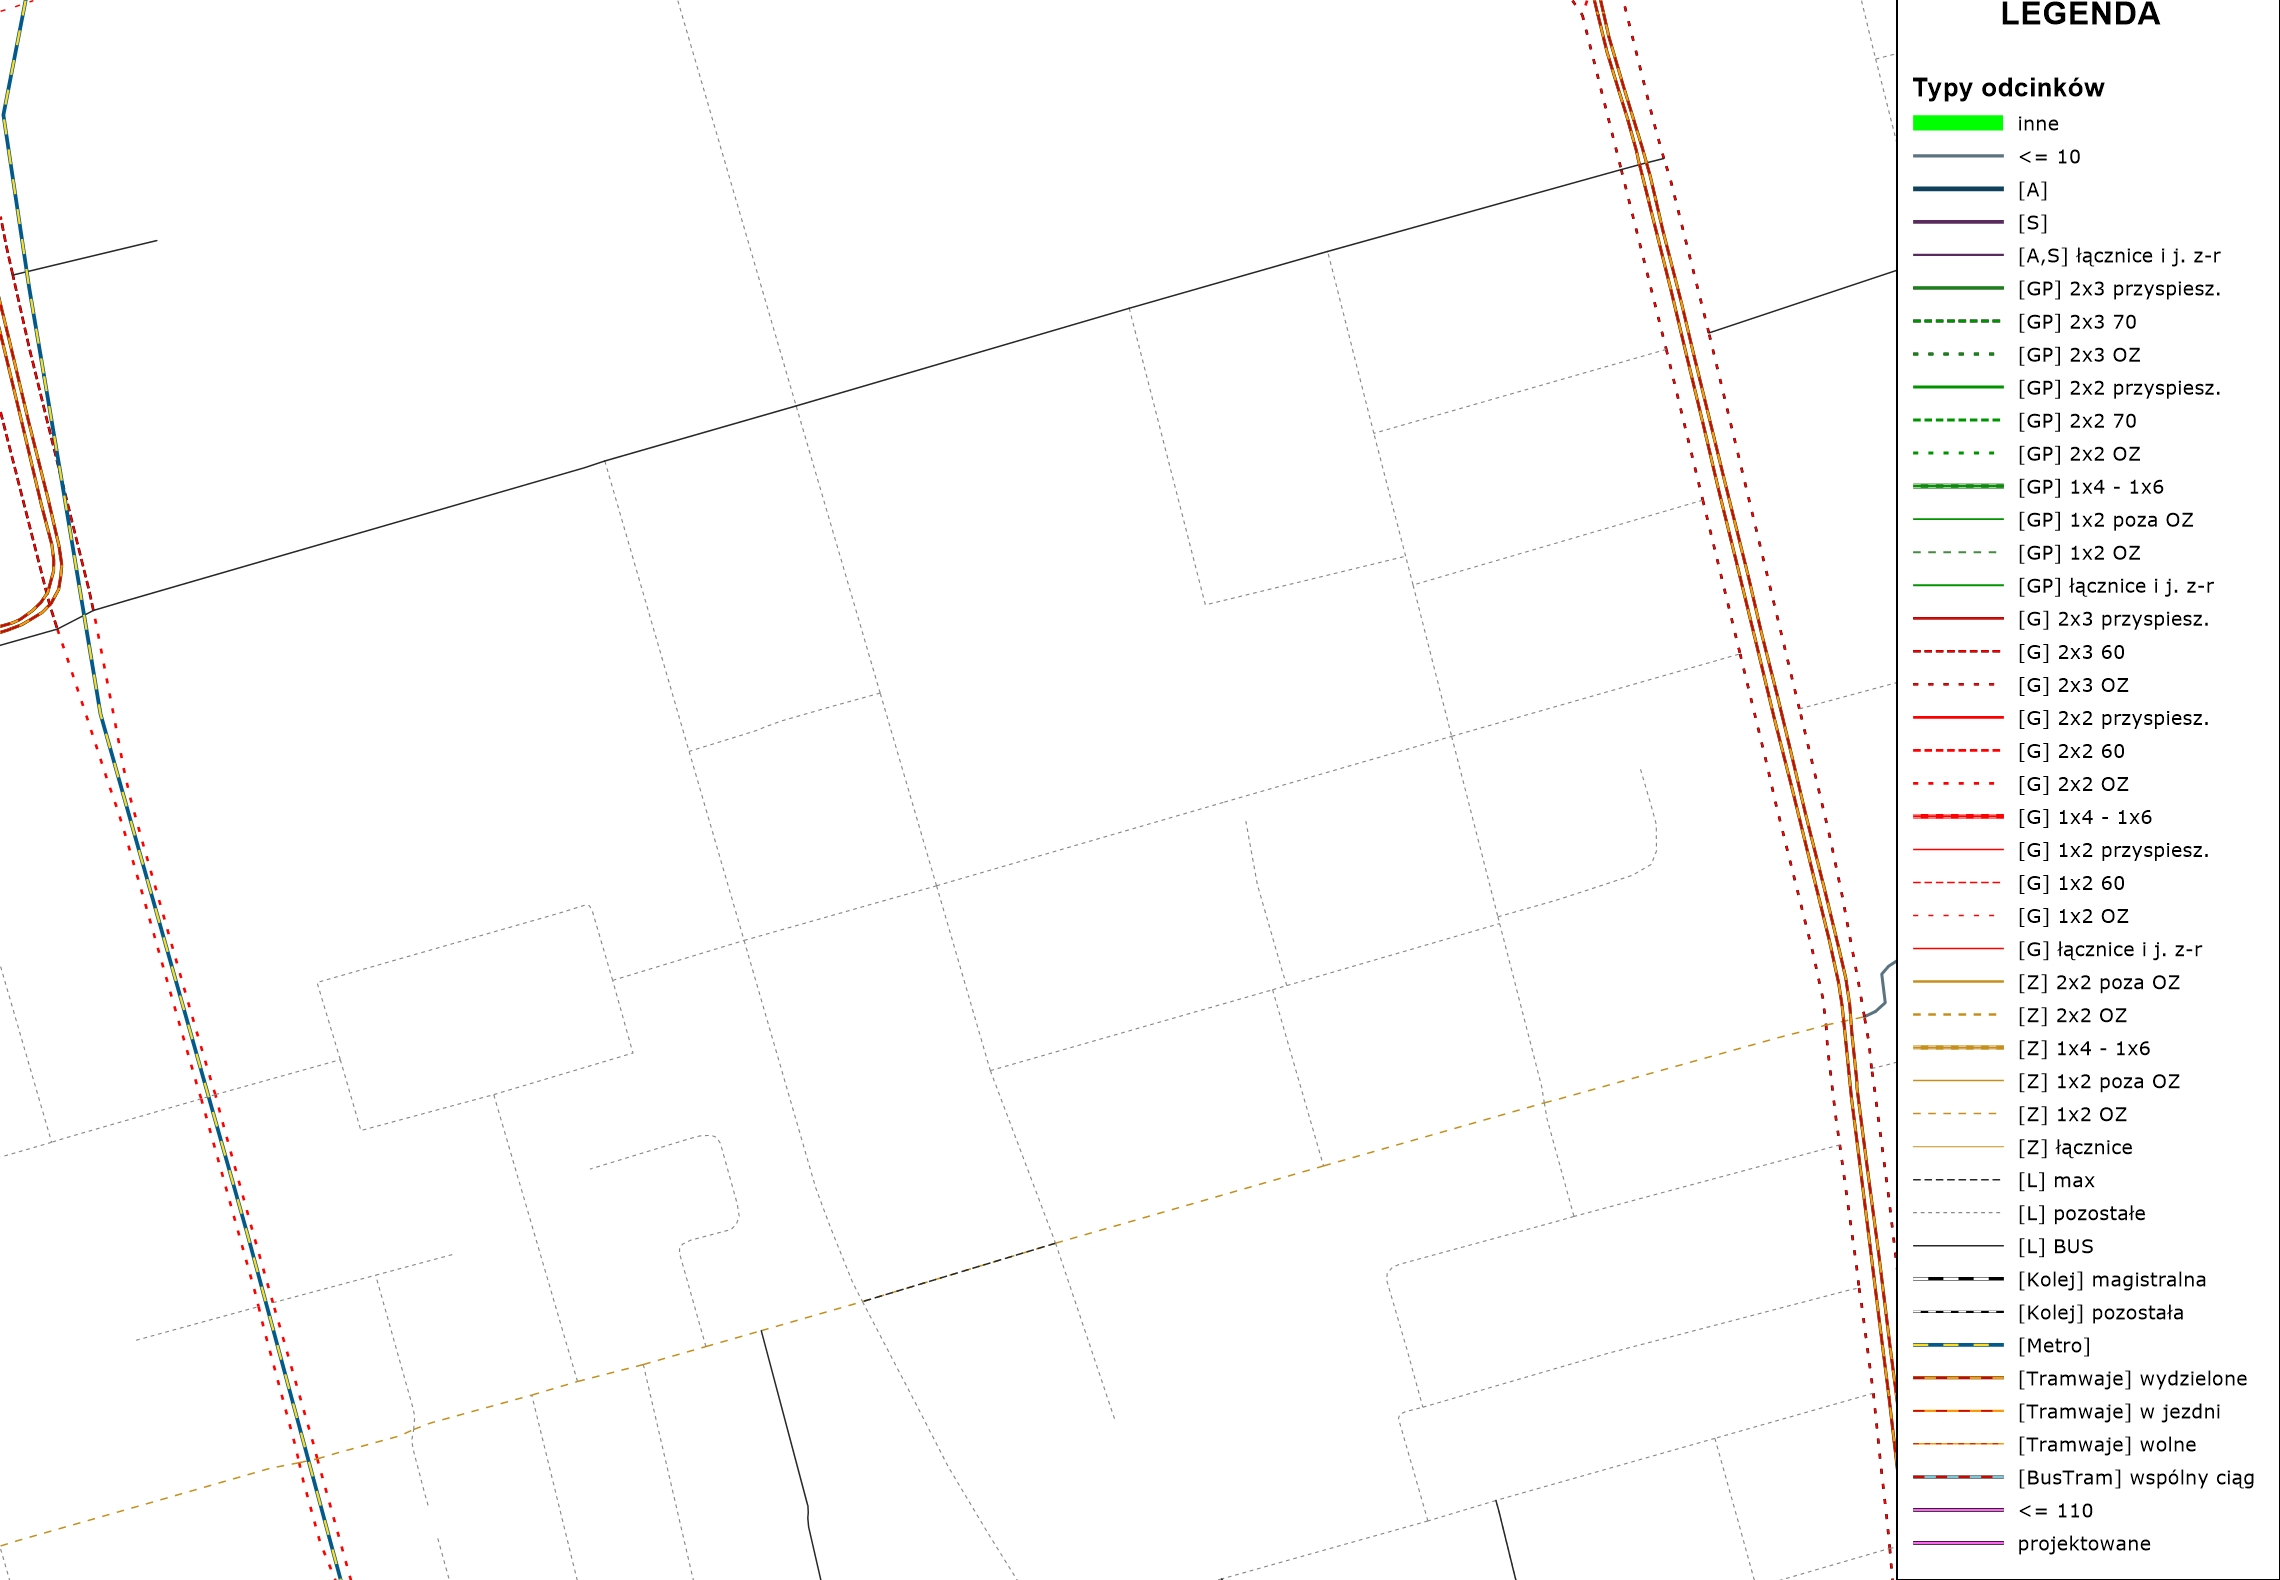
\includegraphics[width=0.9\textwidth]{local_roads}
 \end{center}
  \end{figure} 
\end{frame}

\begin{frame}{Odcinki}{węzły drogowe}
\begin{figure}
\begin{center}
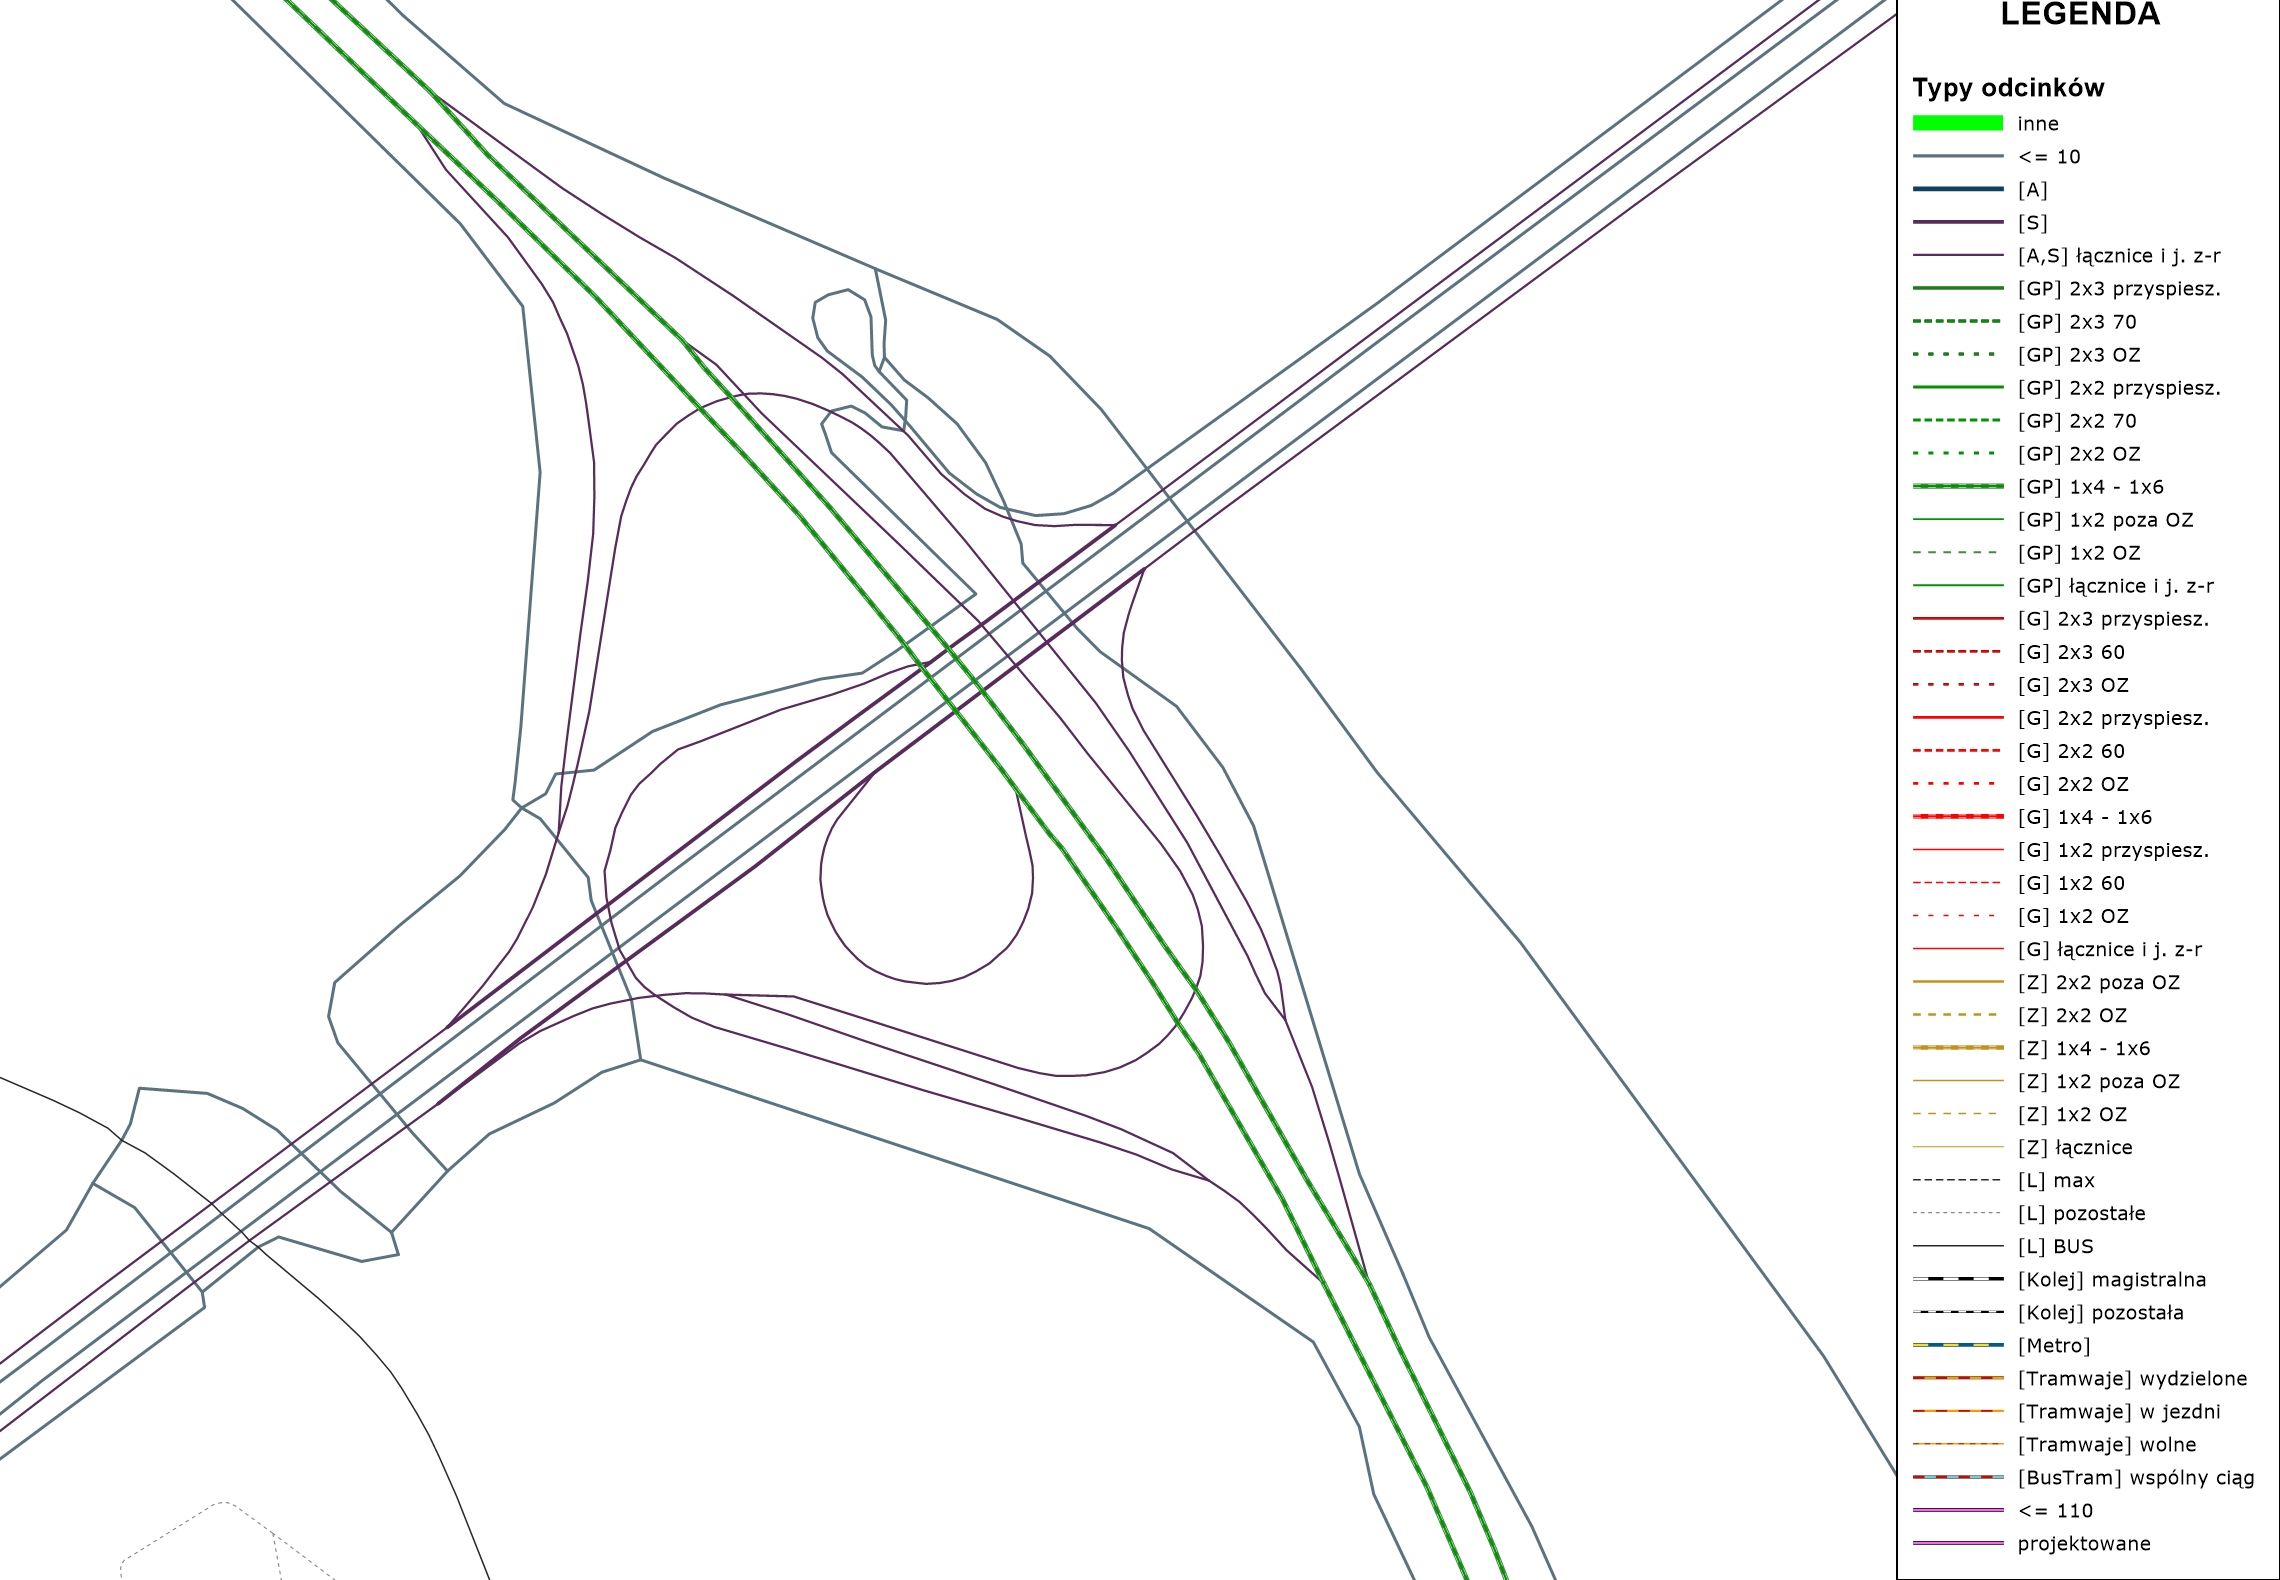
\includegraphics[width=0.9\textwidth]{junction}
 \end{center}
  \end{figure} 
\end{frame}


\begin{frame}{Odcinki}{inwestycje planowane}
\begin{figure}
\begin{center}
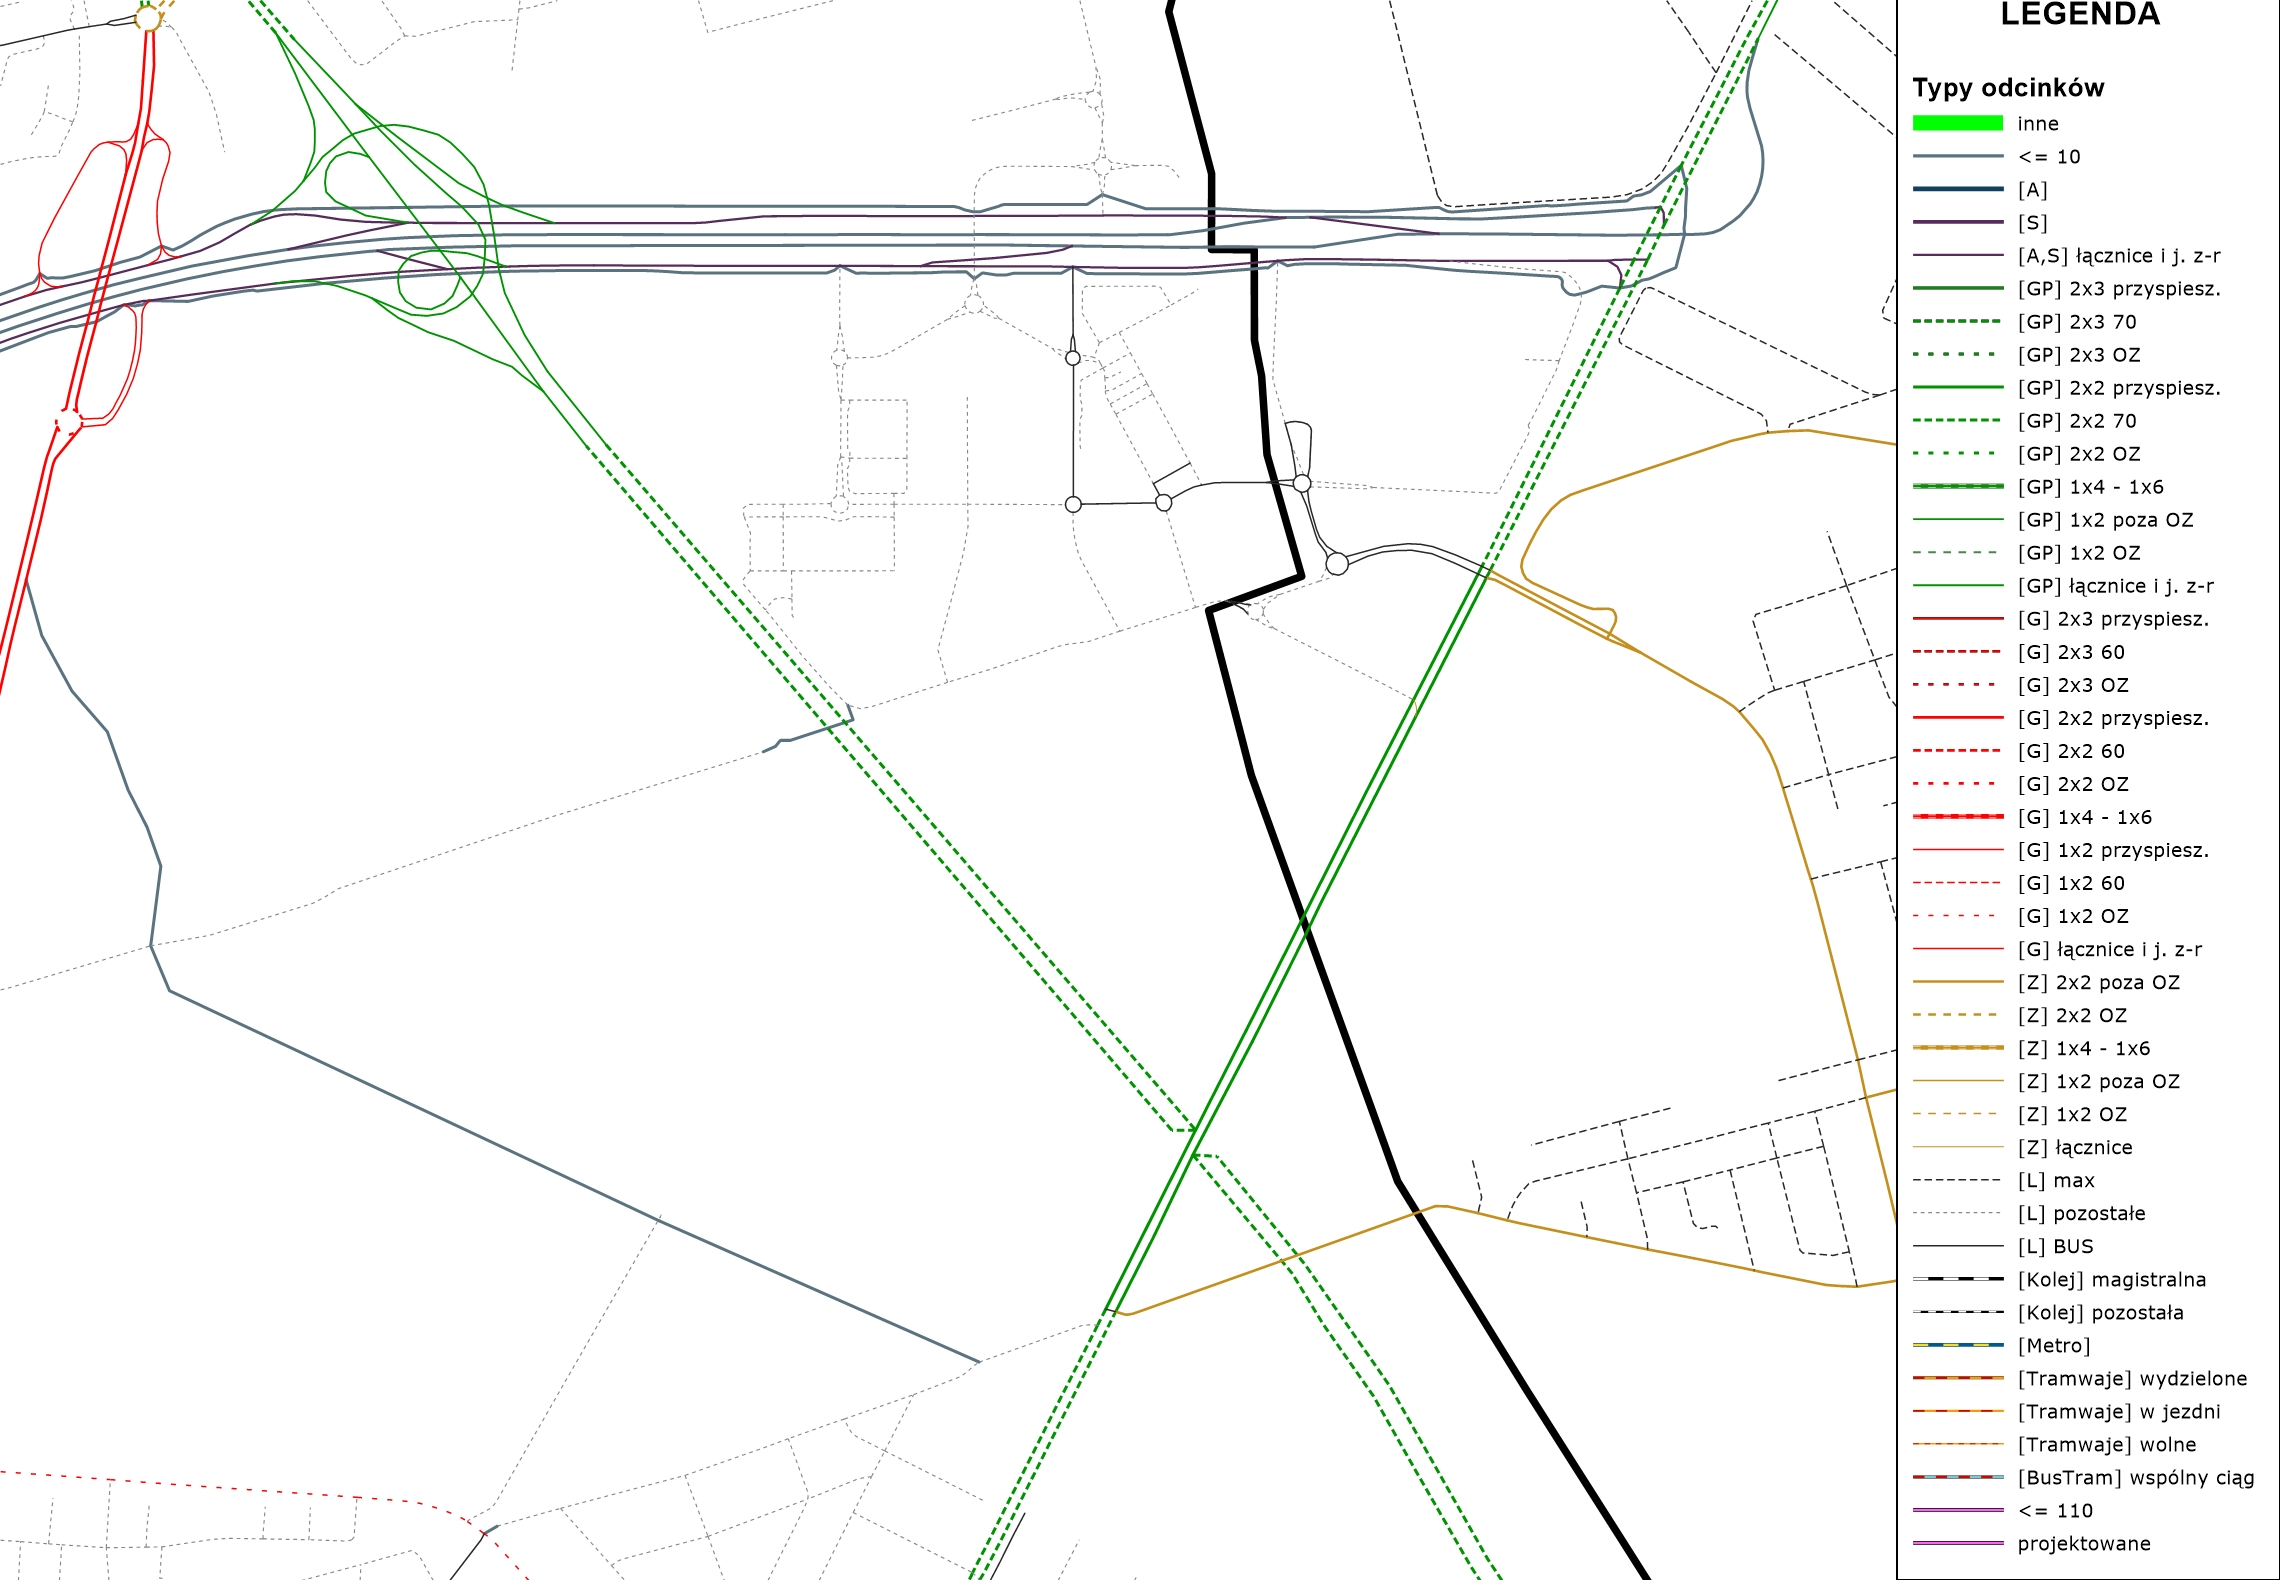
\includegraphics[width=0.9\textwidth]{planned}
 \end{center}
  \end{figure} 
\end{frame}


\begin{frame}{Odcinki}{kolej}
\begin{figure}
\begin{center}
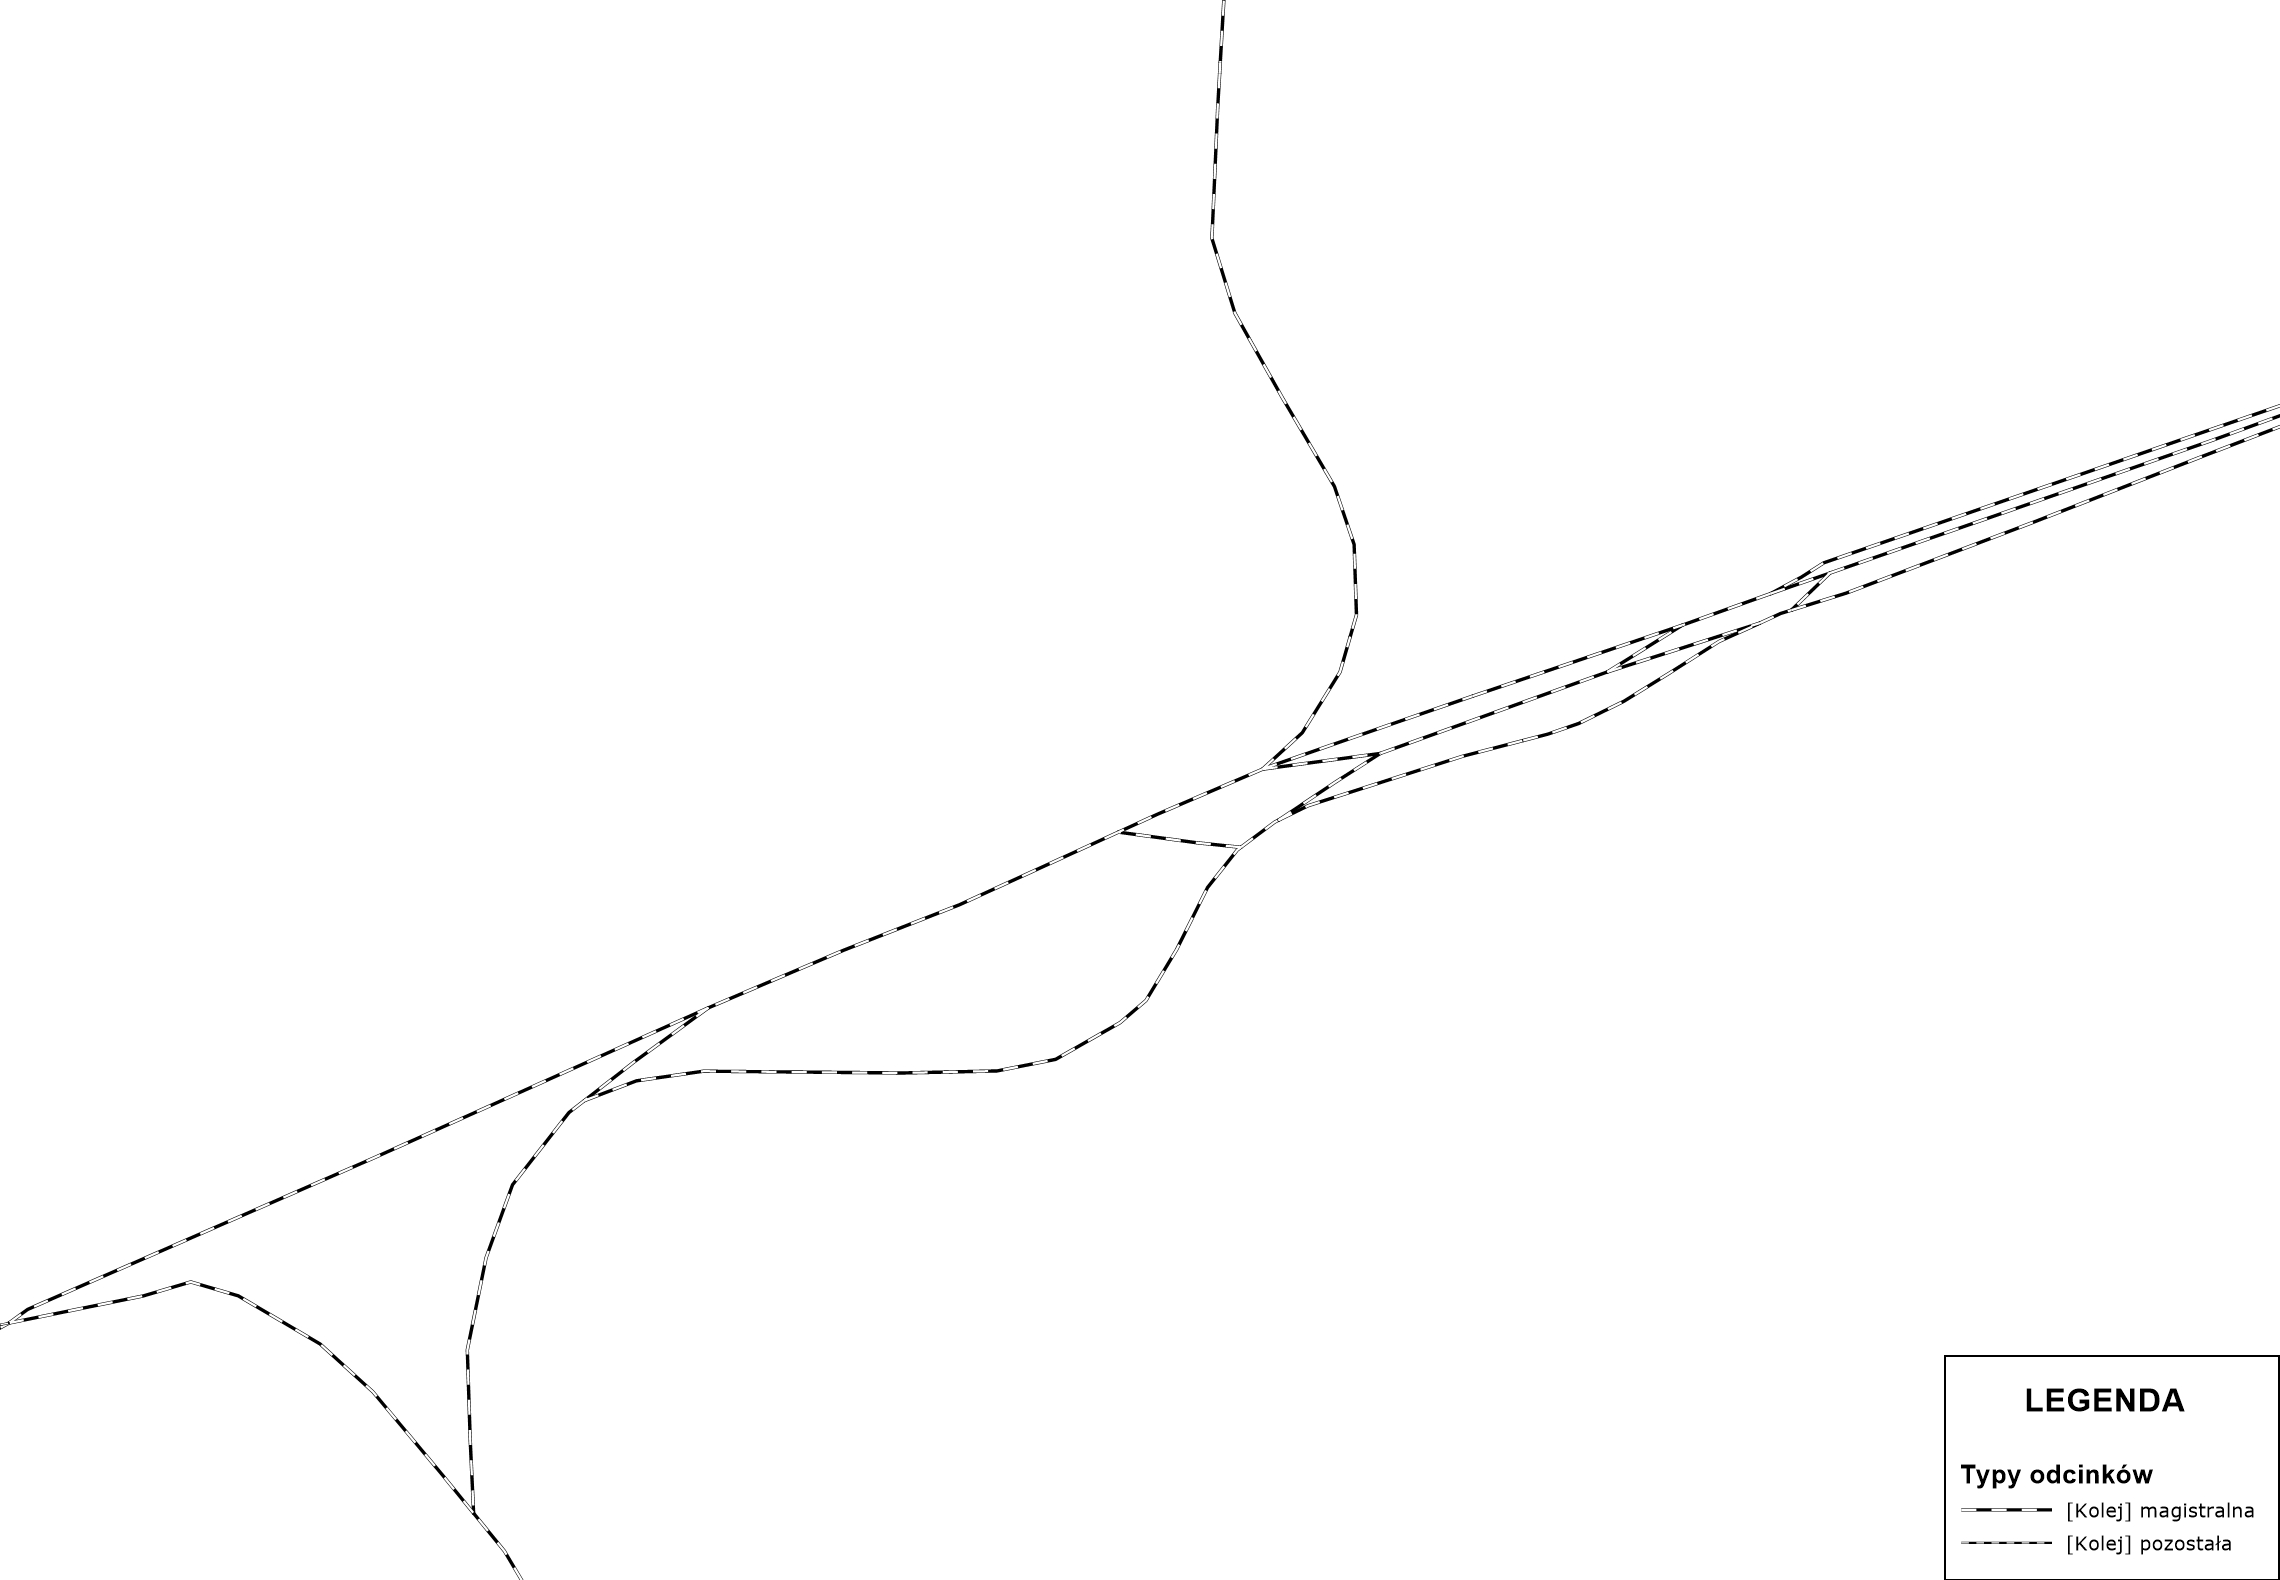
\includegraphics[width=0.9\textwidth]{rail}
 \end{center}
  \end{figure} 
\end{frame}

\begin{frame}{Odcinki}{metro}
\begin{figure}
\begin{center}
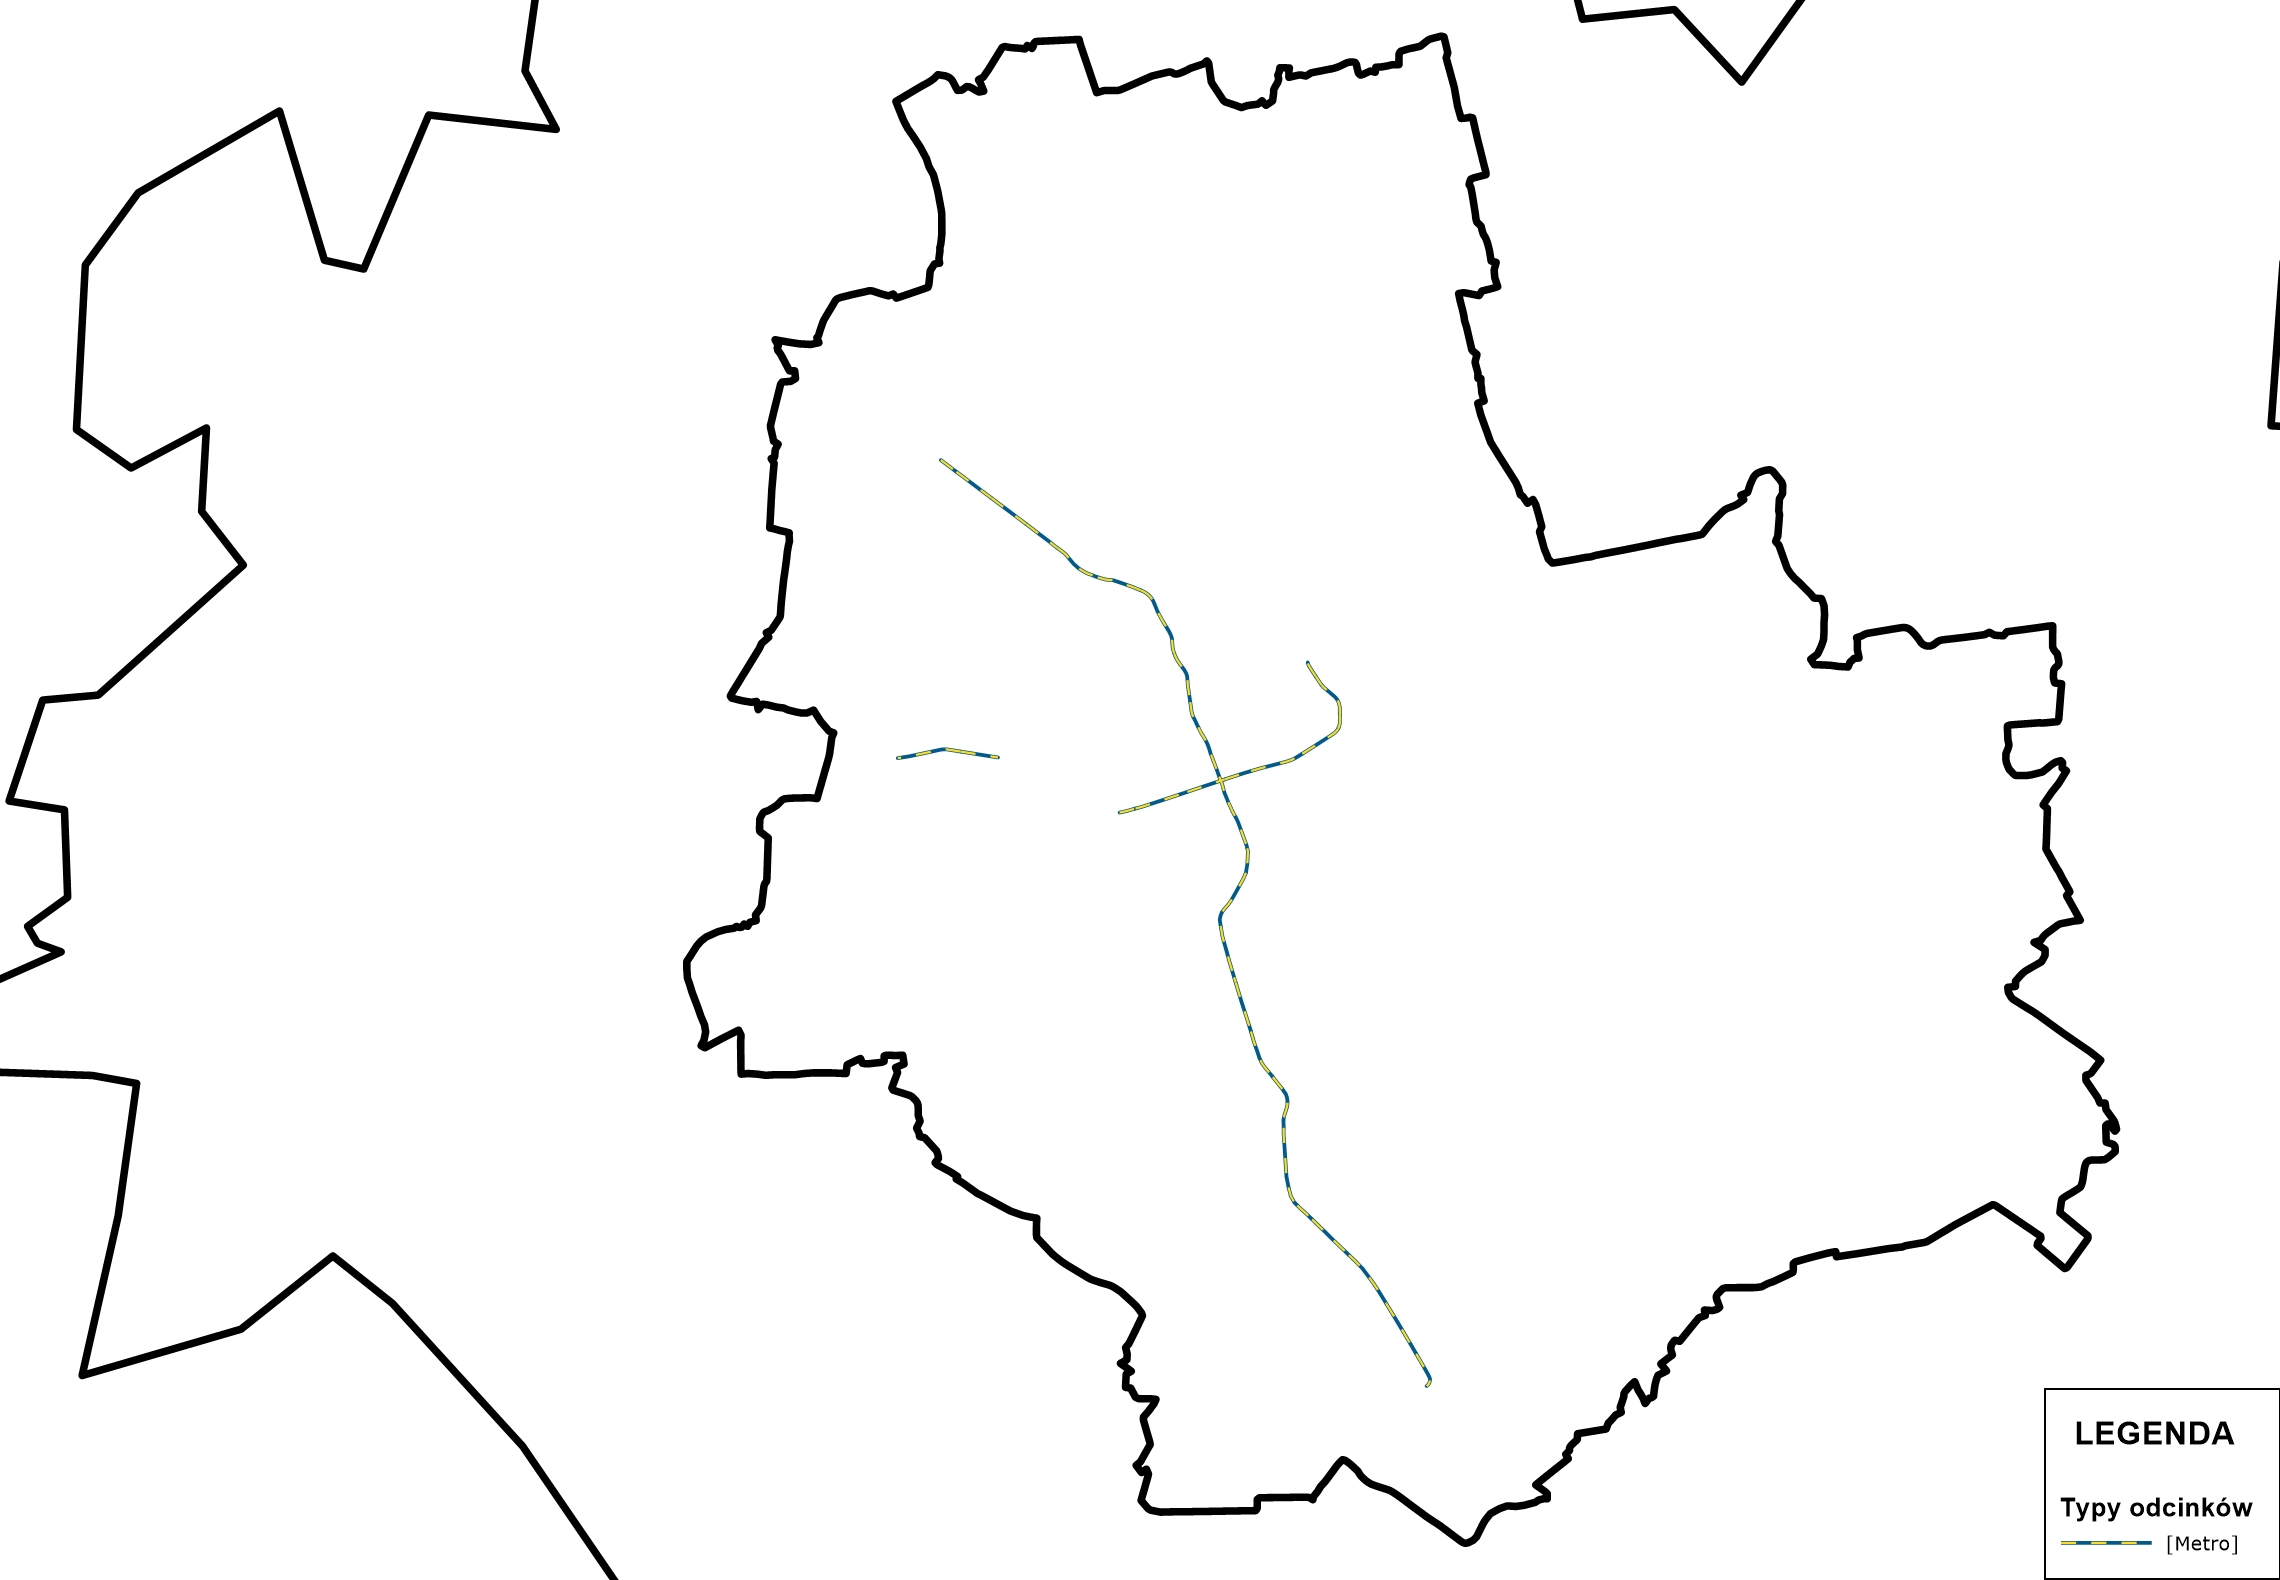
\includegraphics[width=0.9\textwidth]{metro}
 \end{center}
  \end{figure} 
\end{frame}

\begin{frame}{Odcinki}{tramwaj}
\begin{figure}
\begin{center}
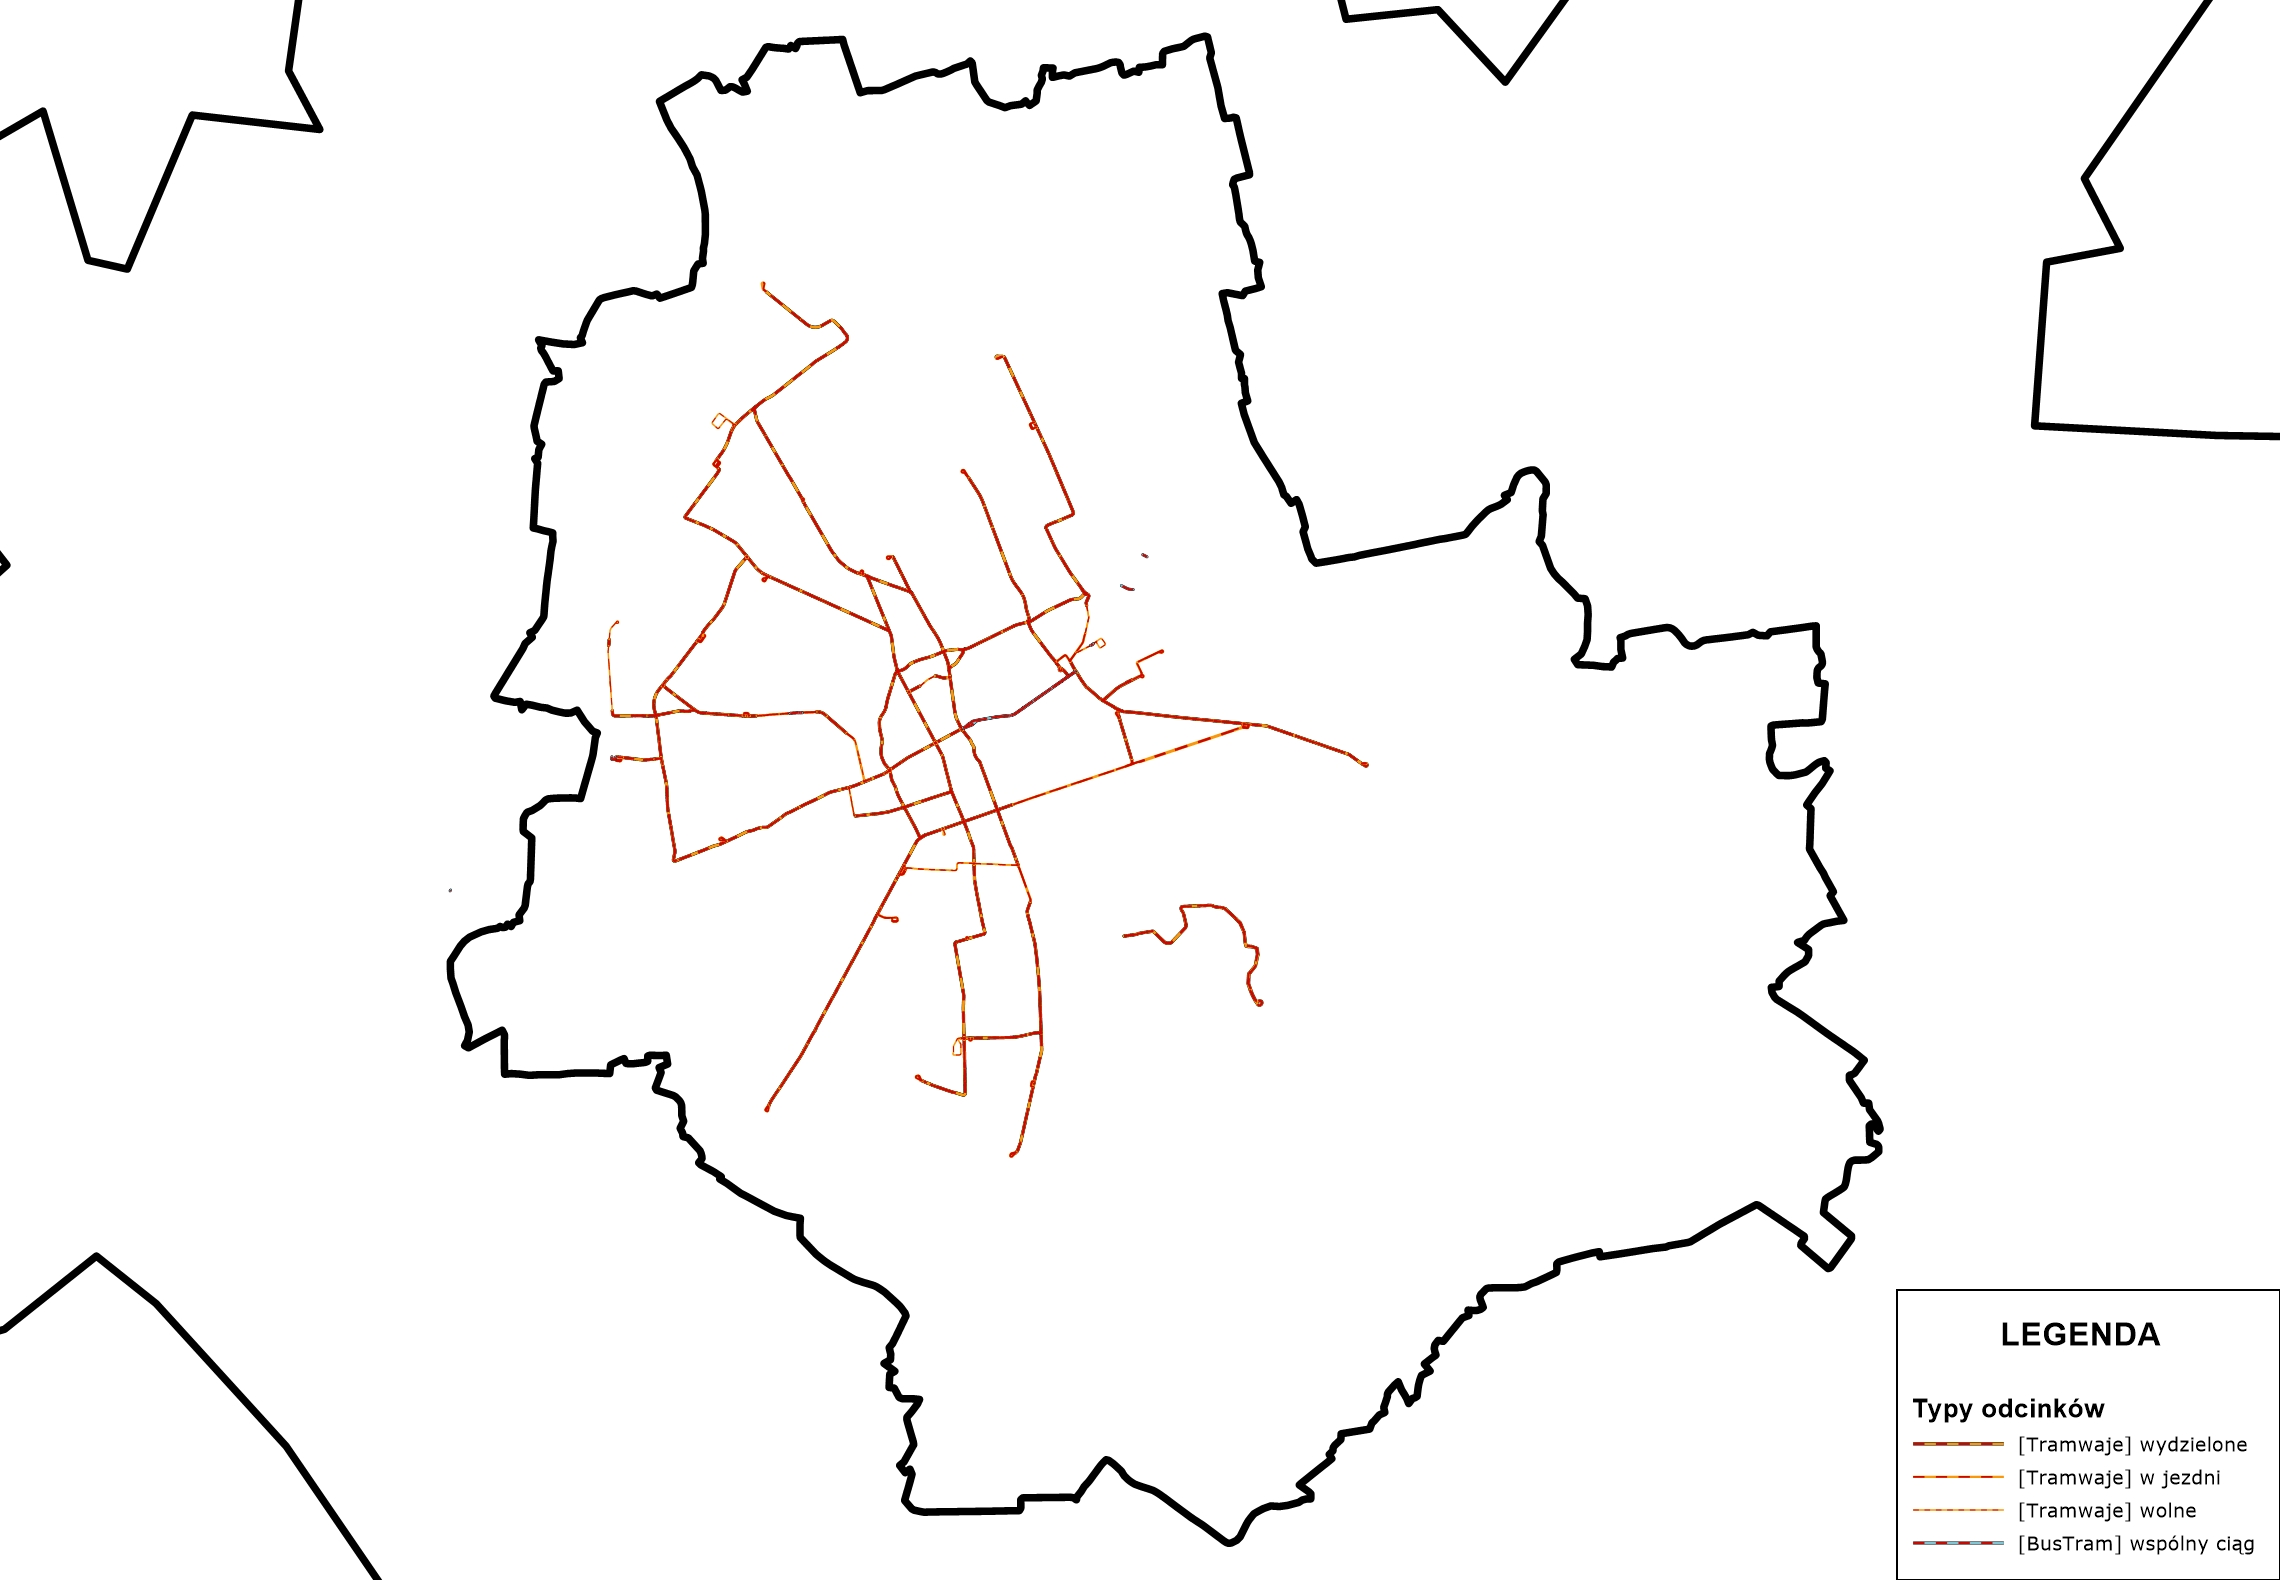
\includegraphics[width=0.9\textwidth]{tram}
 \end{center}
  \end{figure} 
\end{frame}

\begin{frame}{Odcinki}{układ torowy}
\begin{figure}
\begin{center}
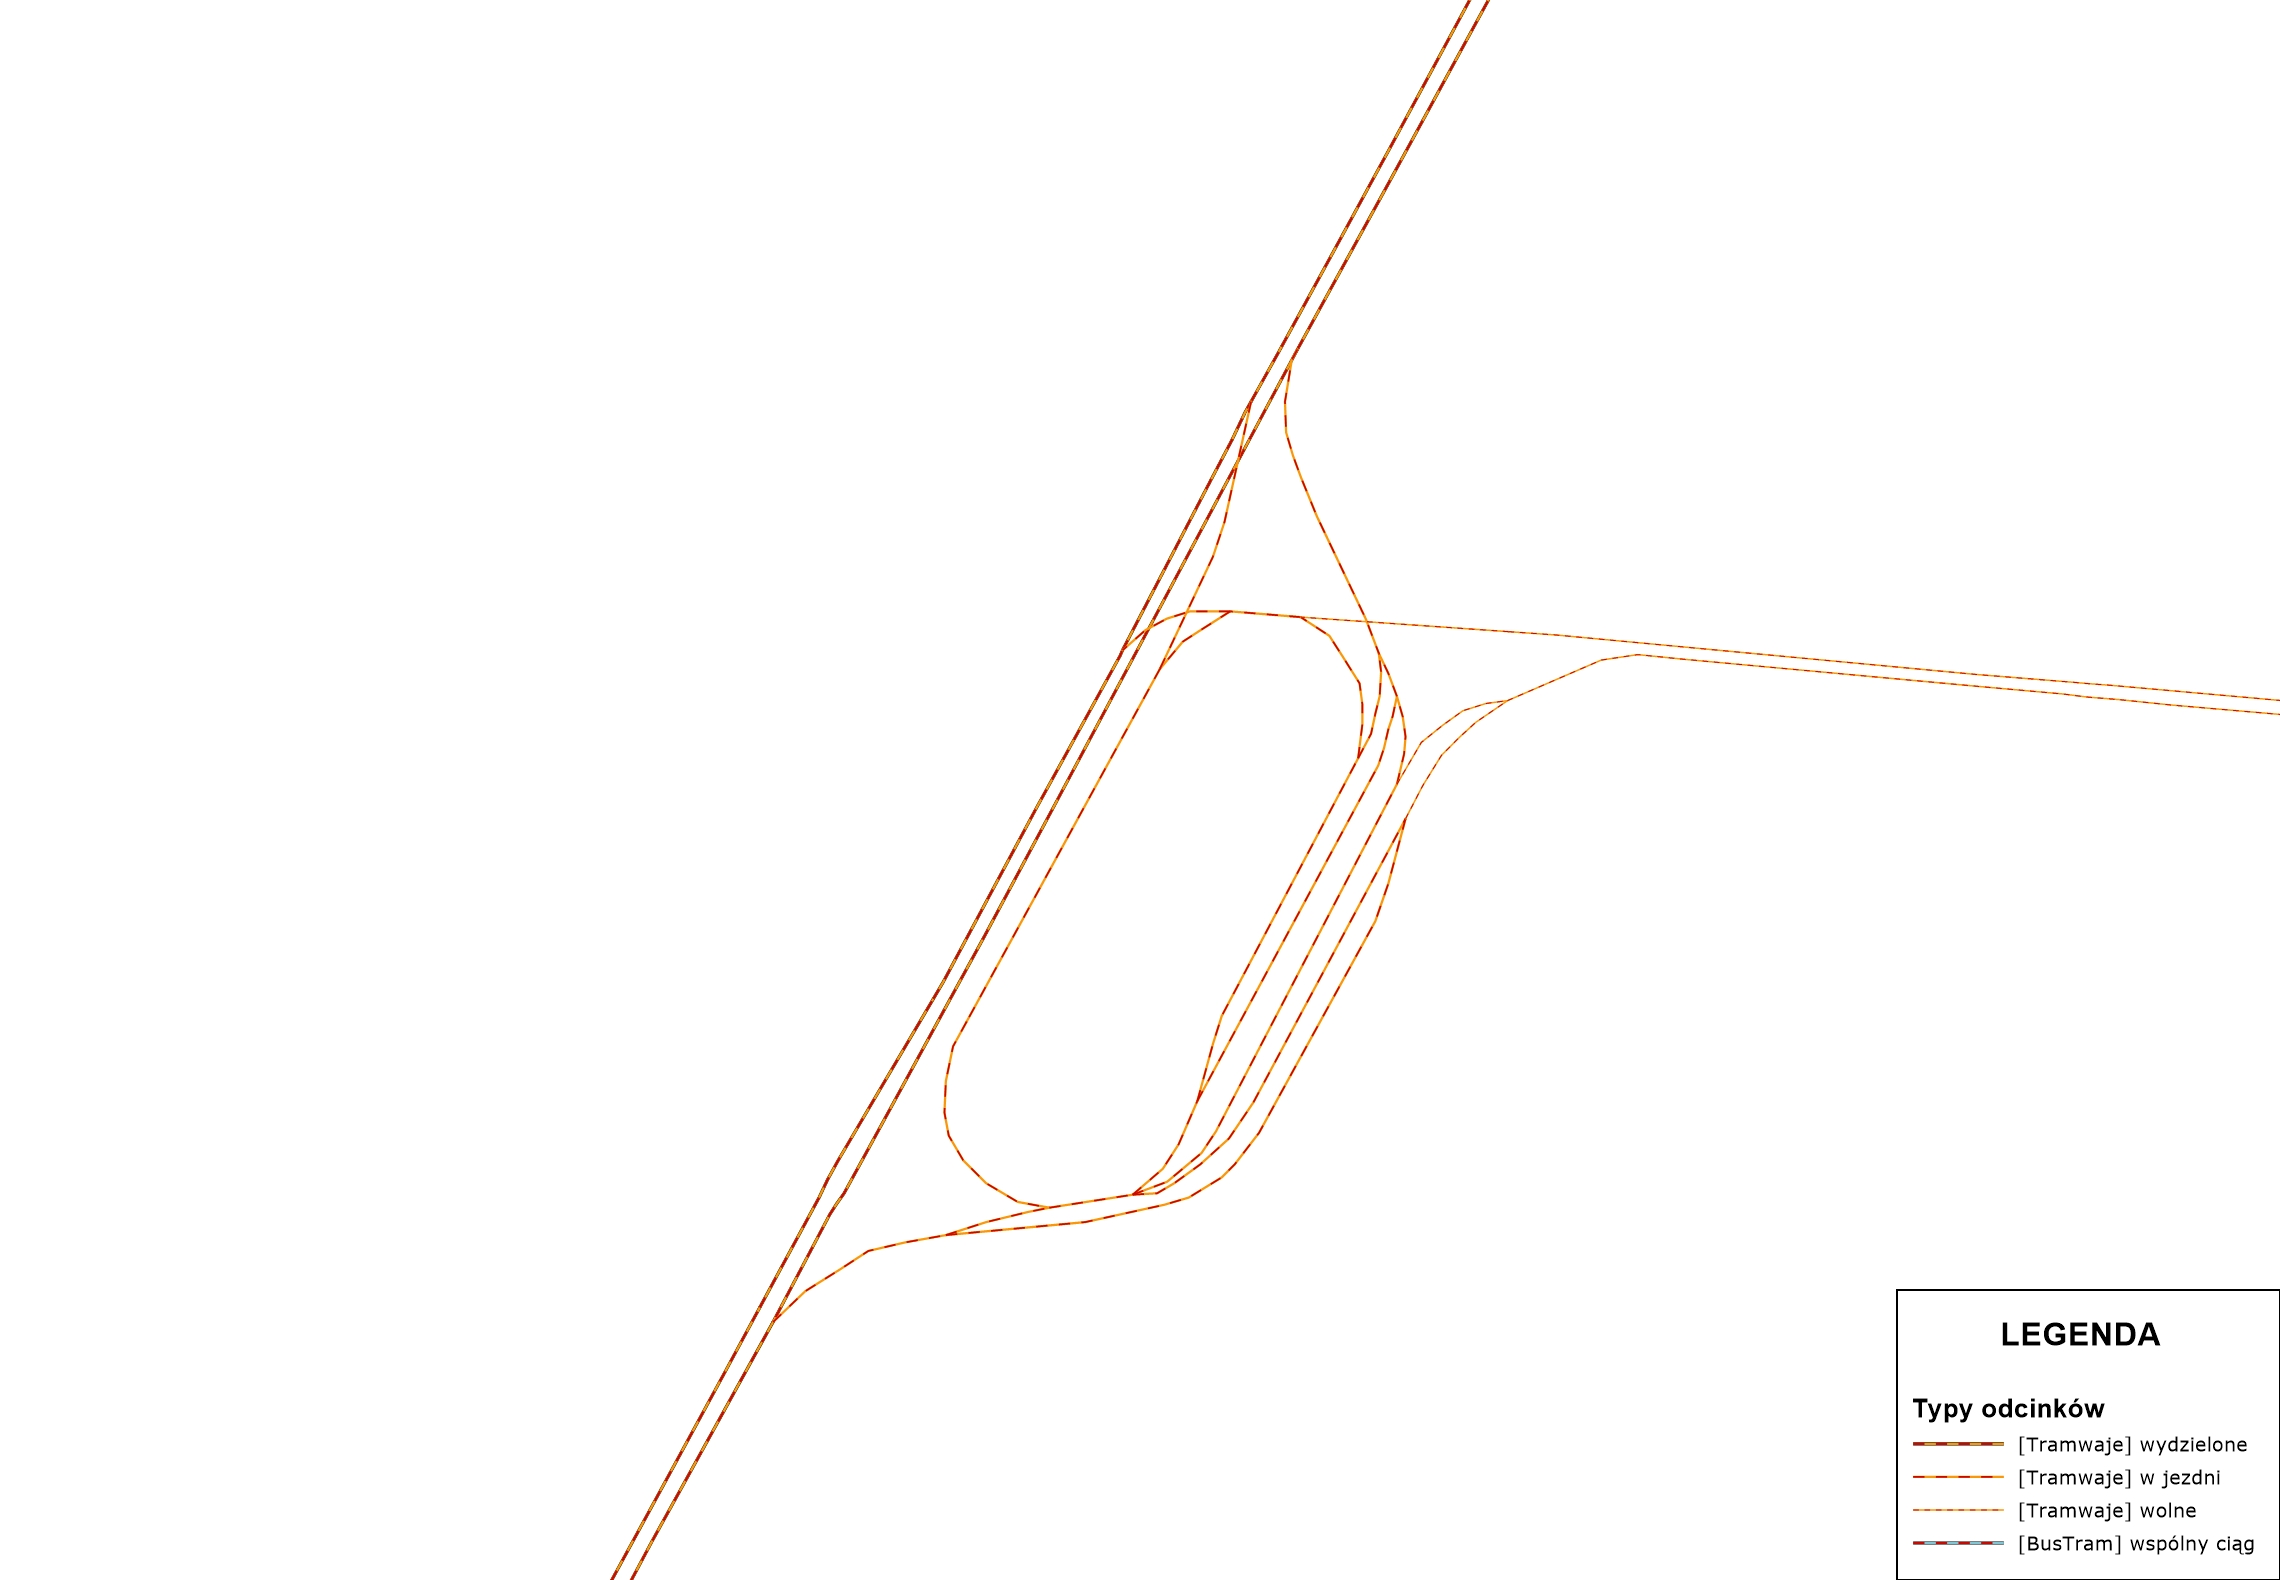
\includegraphics[width=0.9\textwidth]{tram2}
 \end{center}
  \end{figure} 
\end{frame}

\subsection{Sieć komunikacji zbiorowej}
\begin{frame}{Przystanki}
\begin{figure}
\begin{center}
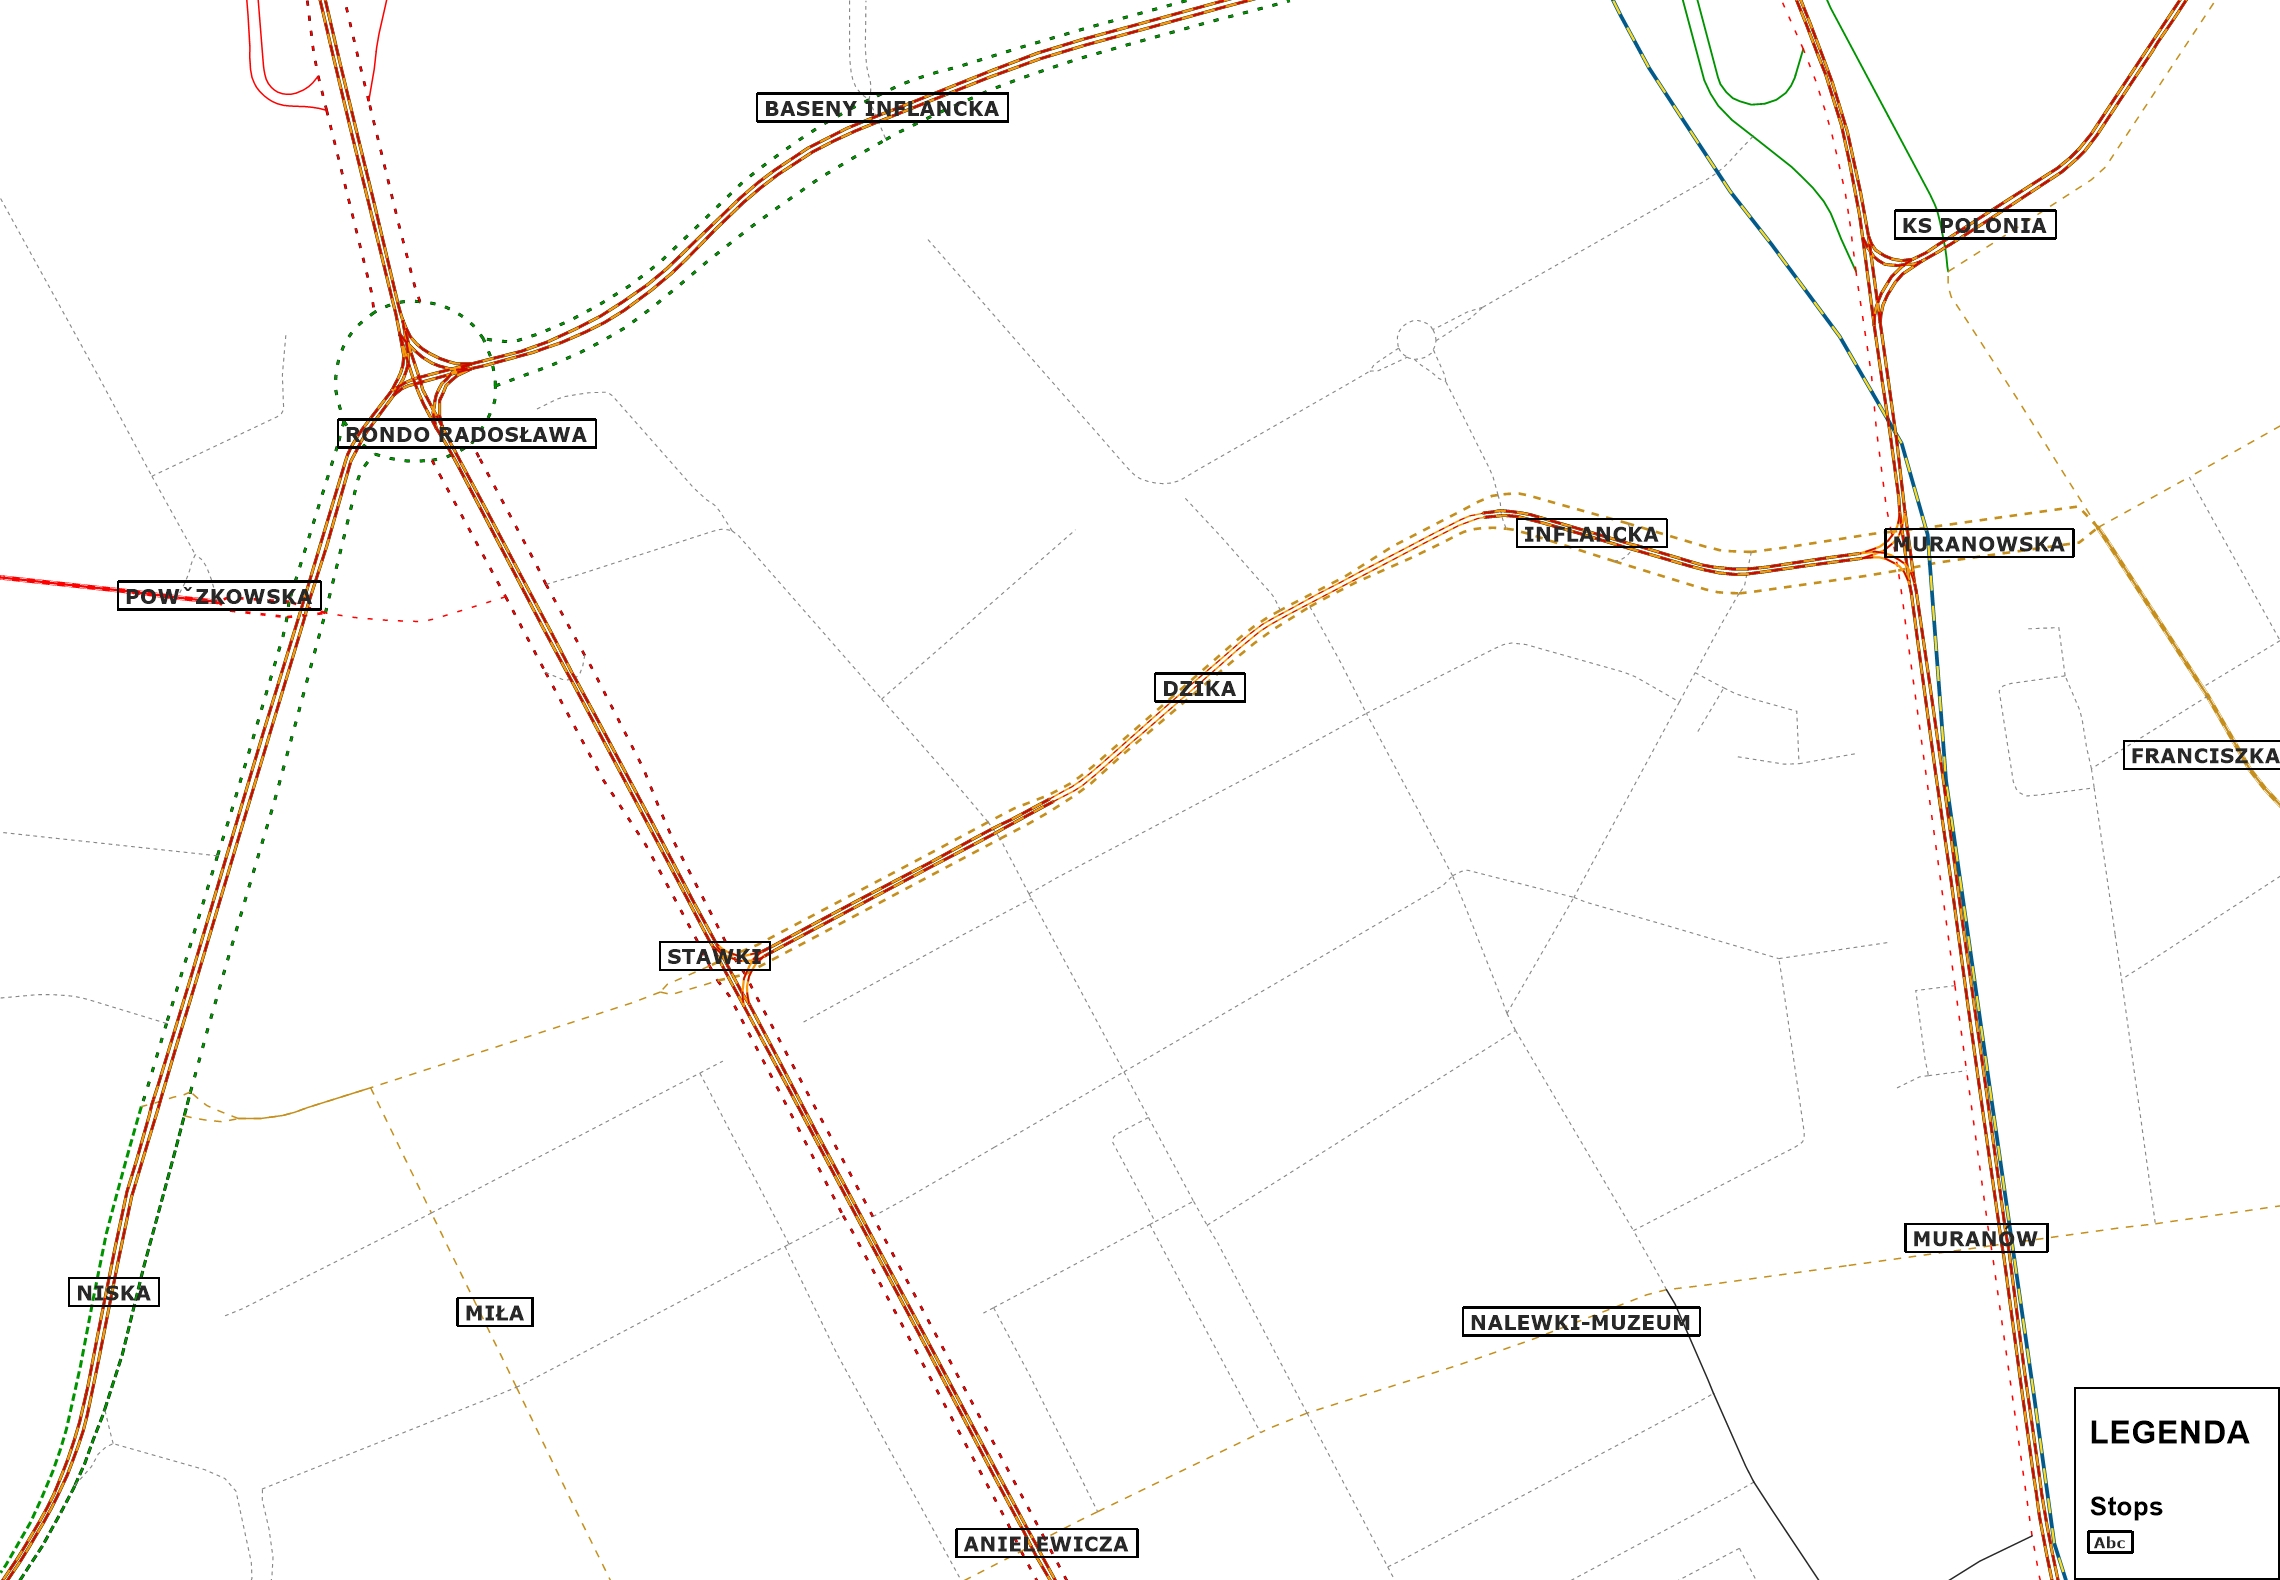
\includegraphics[width=0.9\textwidth]{stops}
 \end{center}
  \end{figure} 
\end{frame}

\begin{frame}{Przystanki}{Zespoły przystankowe}
\begin{figure}\begin{center}
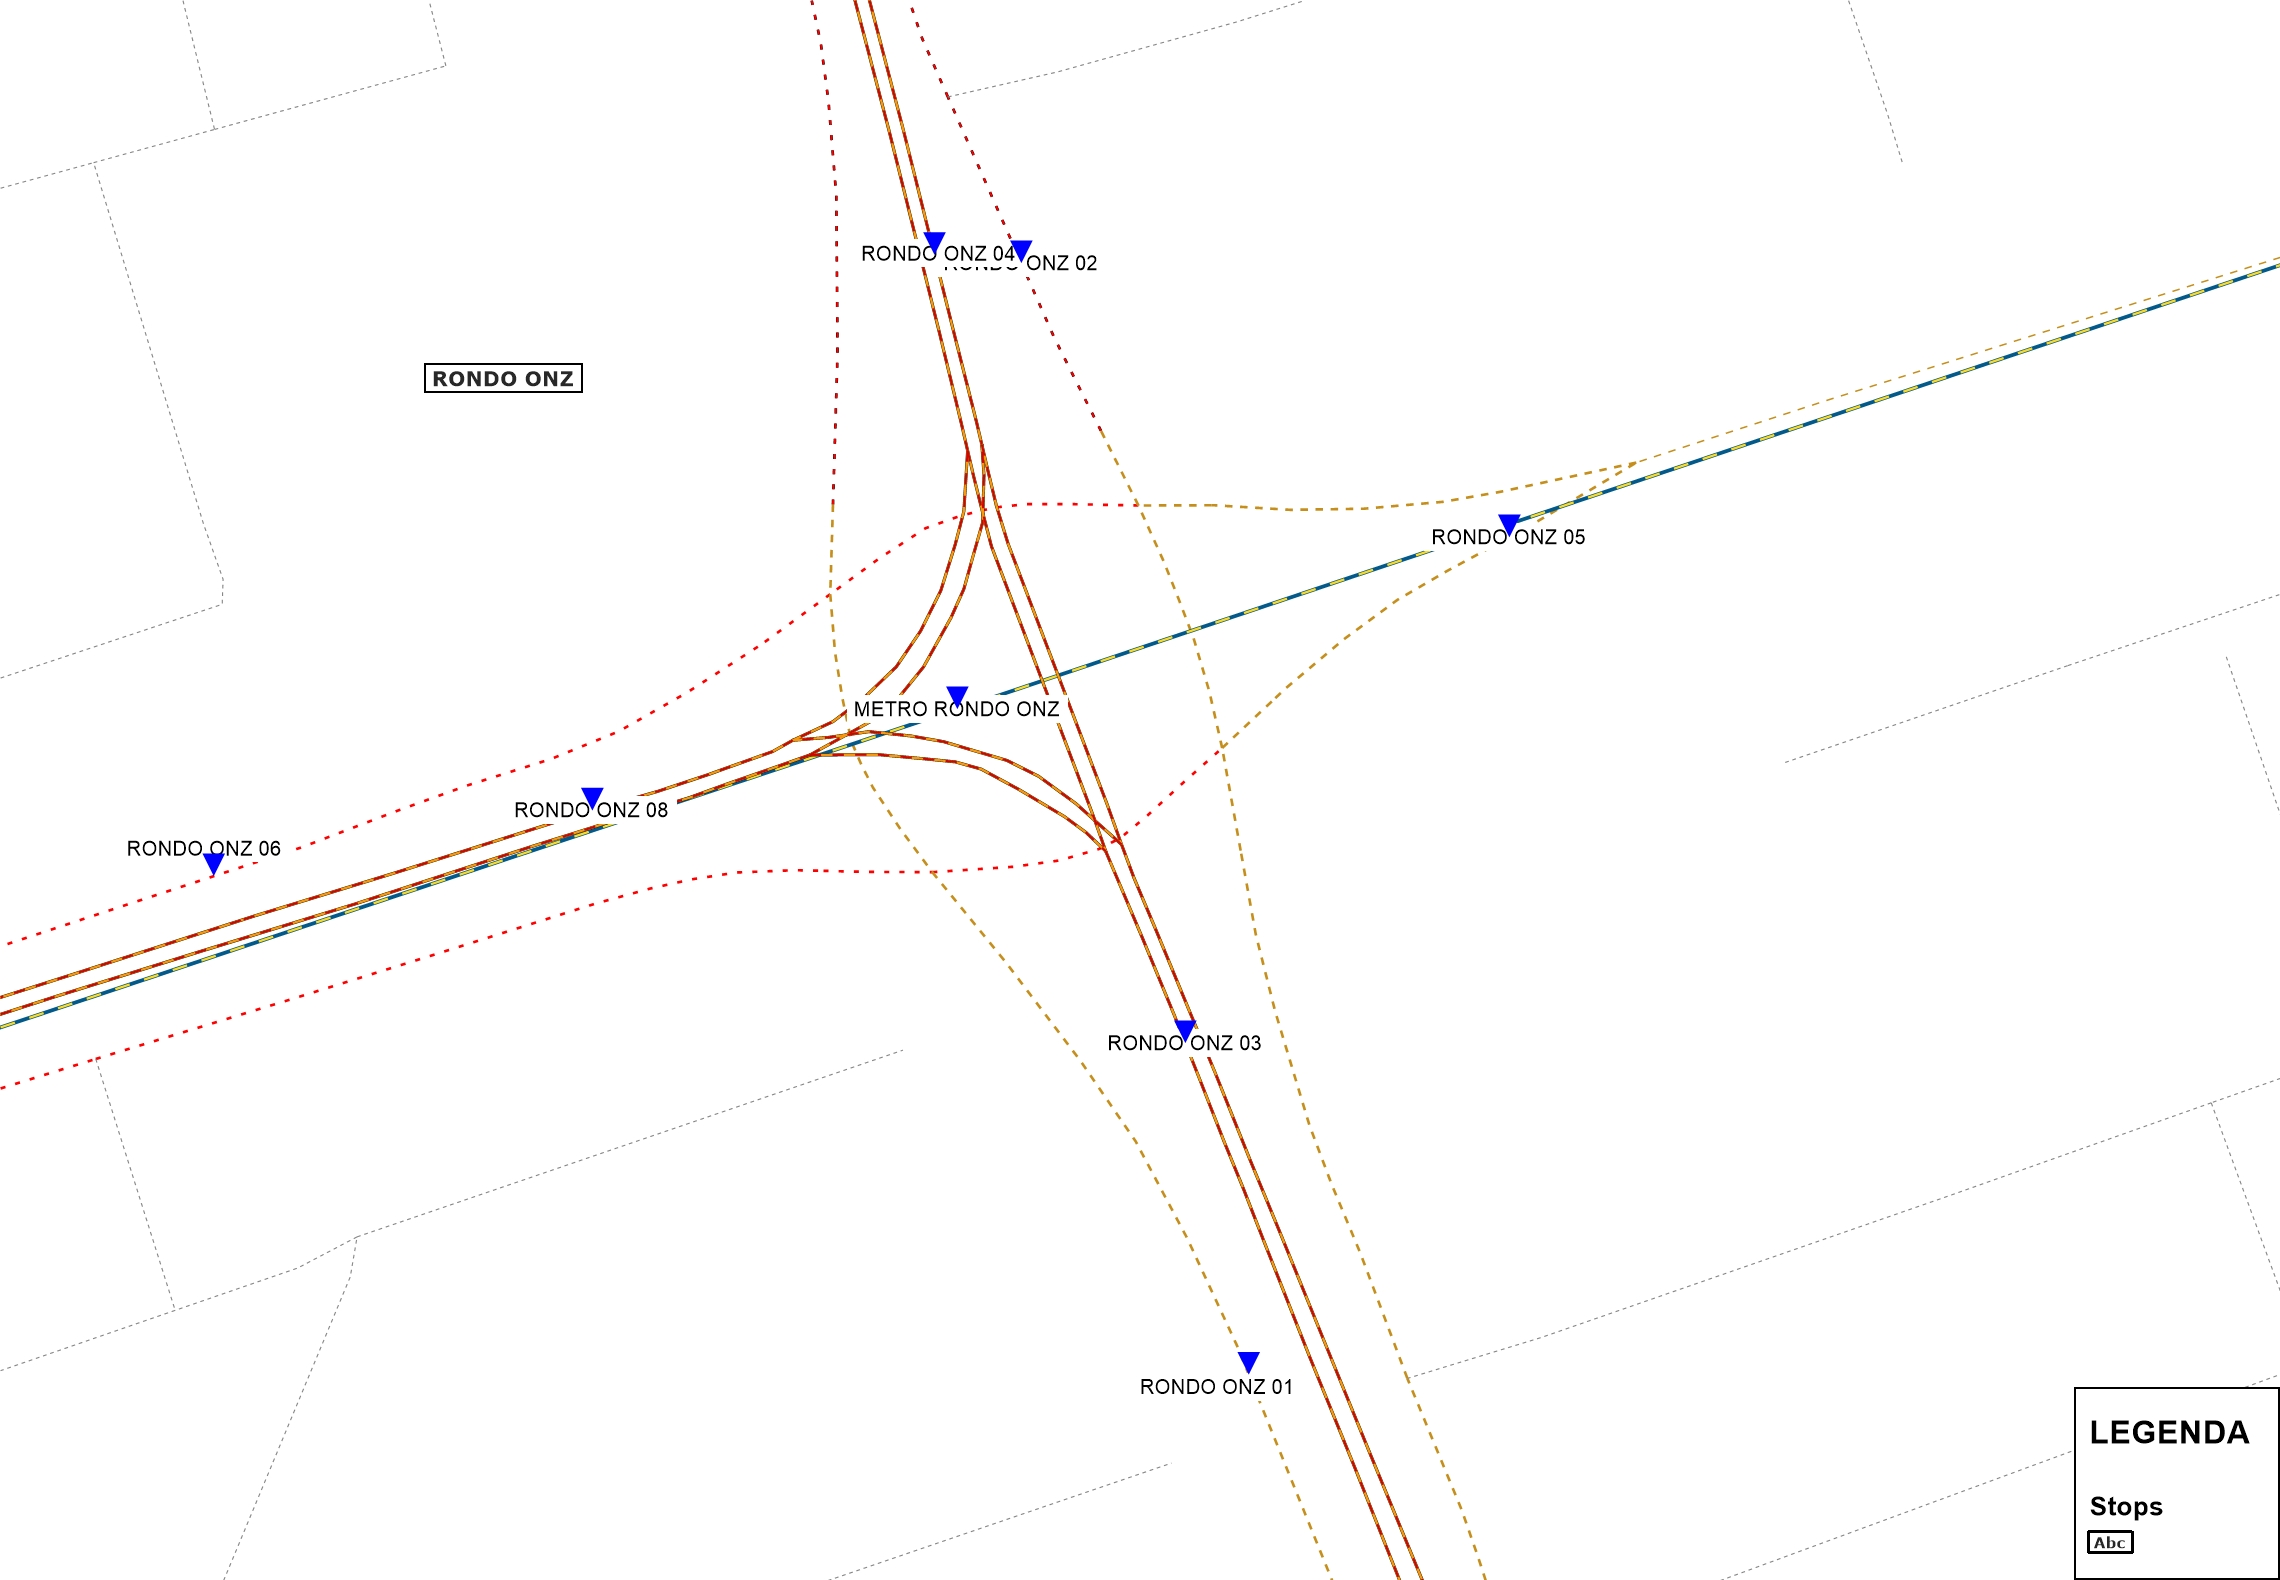
\includegraphics[width=0.9\textwidth]{stop_points}
 \end{center}  \end{figure} 
\end{frame}

\begin{frame}{Przystanki}{Zespoły przystankowe multimodalne}
\begin{figure}\begin{center}
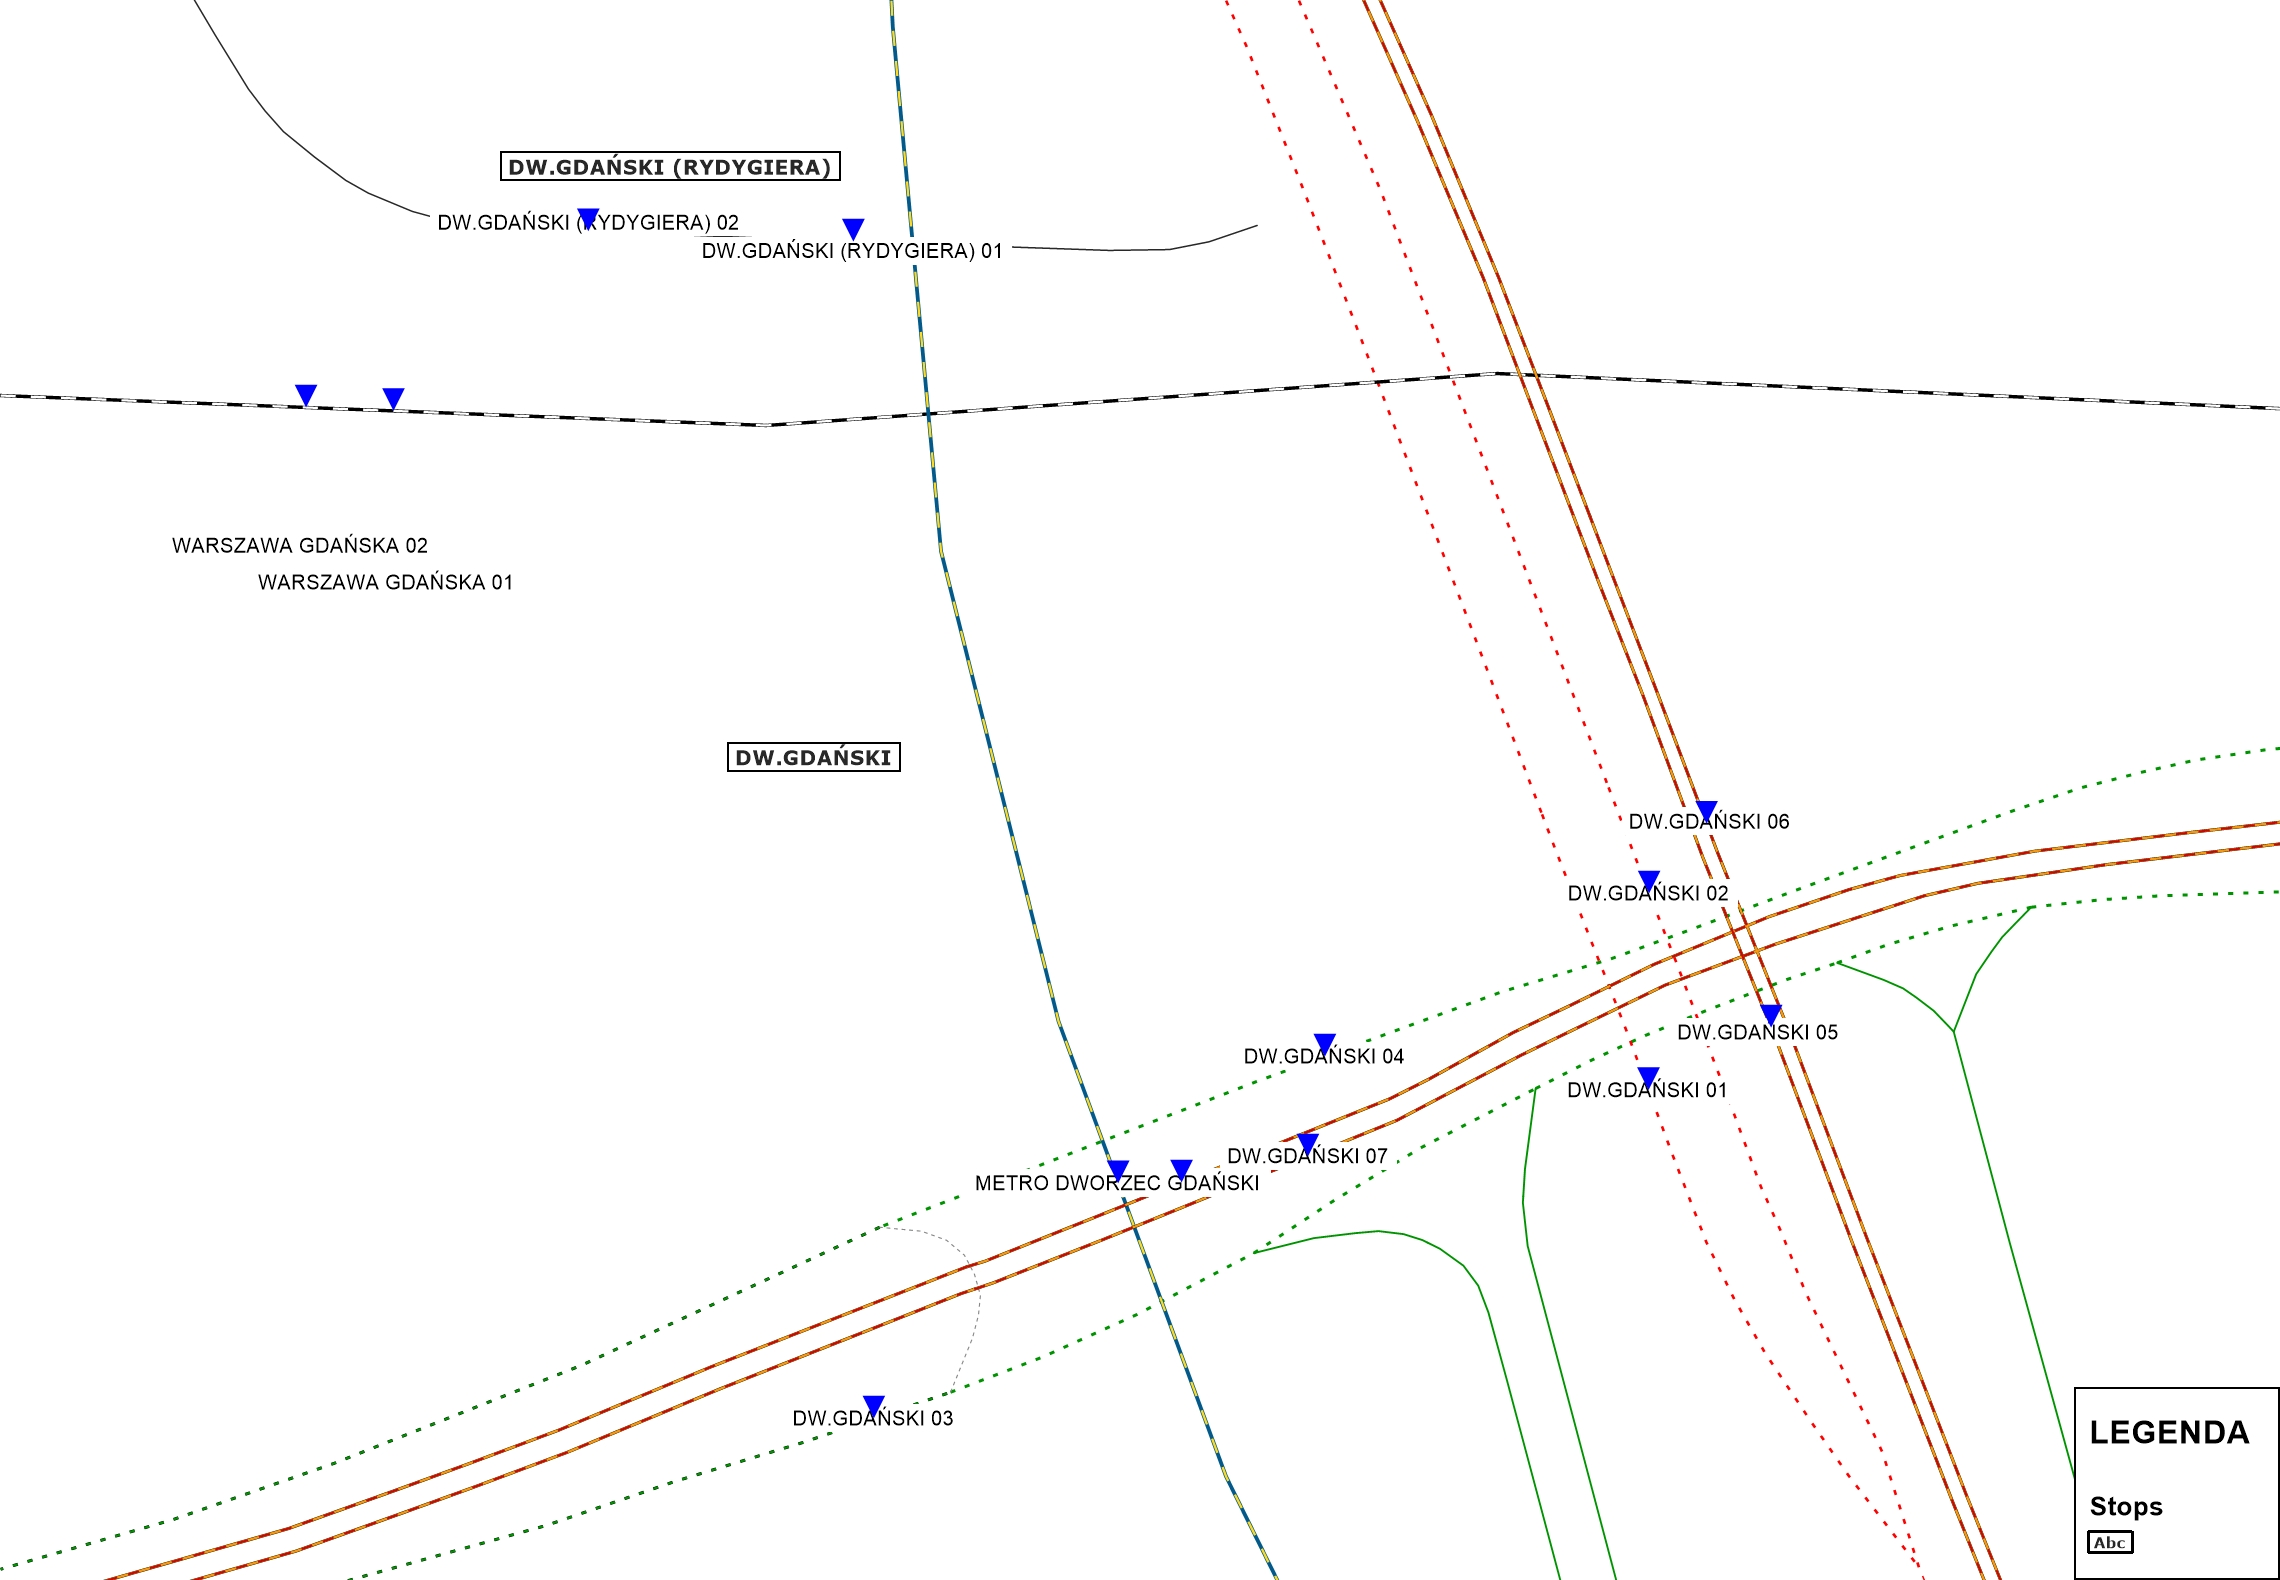
\includegraphics[width=0.9\textwidth]{multi_modal}
 \end{center}  \end{figure} 
\end{frame}

\begin{frame}{Przystanki}{Relacje przesiadkowe - potoki}
\begin{figure}\begin{center}
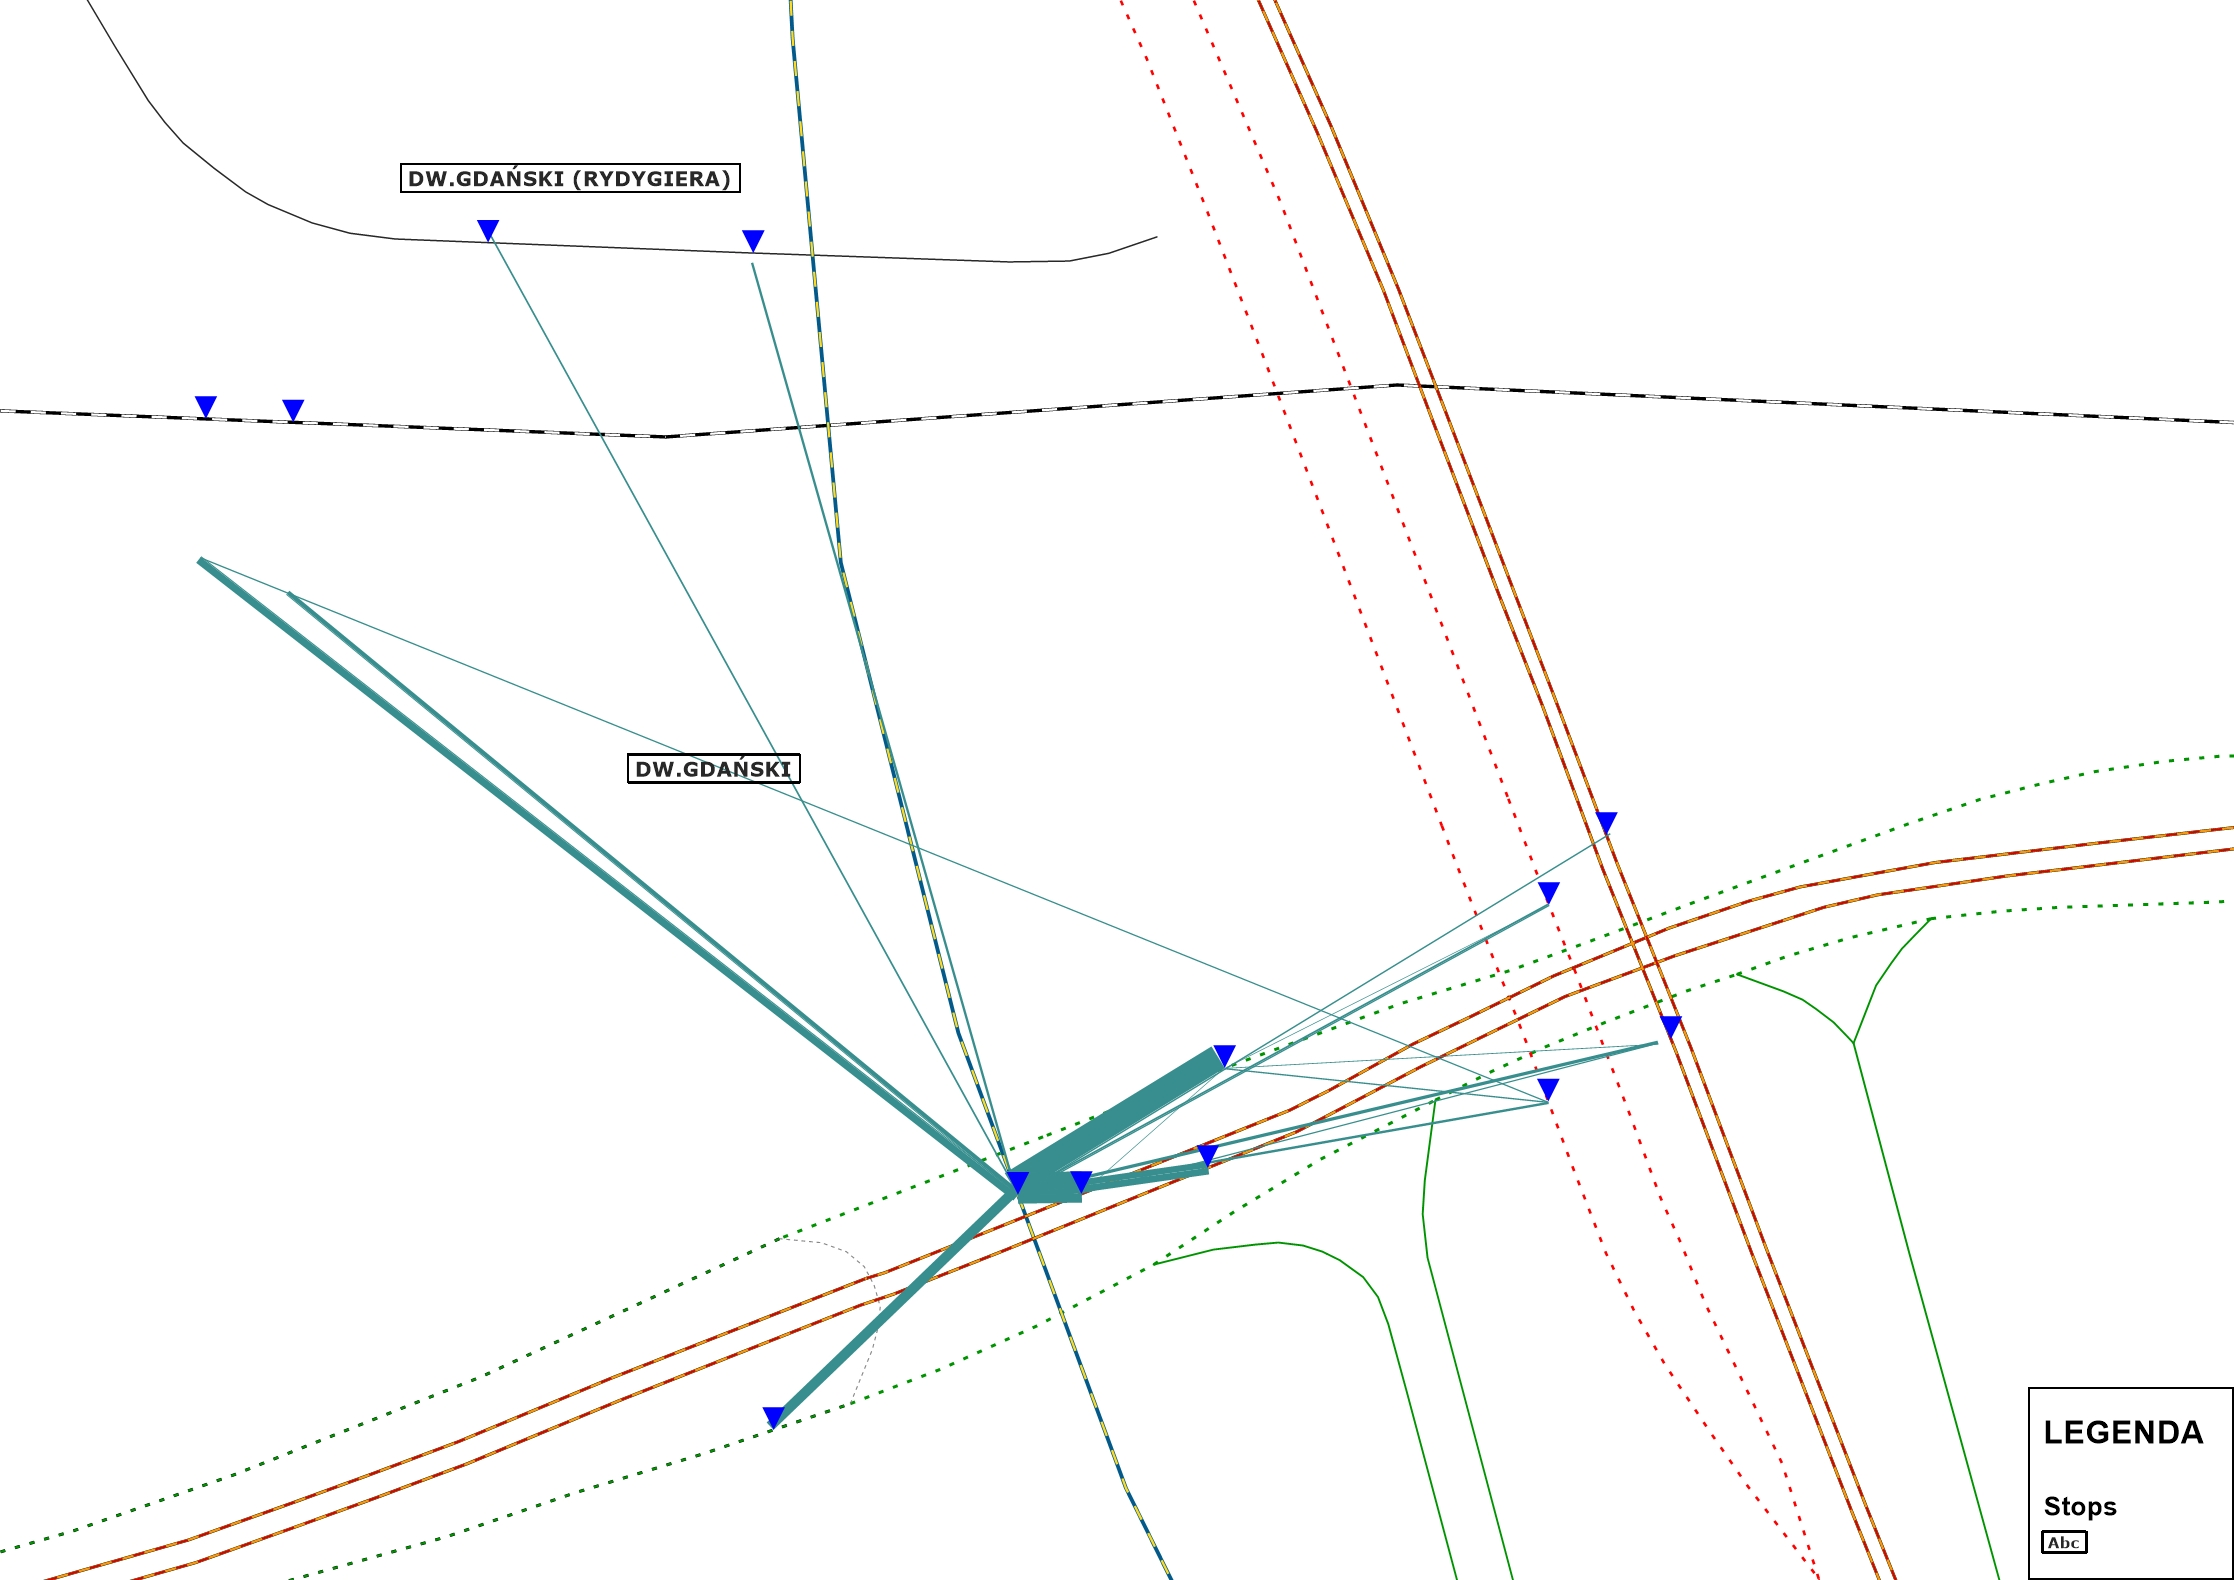
\includegraphics[width=0.9\textwidth]{transfers}
 \end{center}  \end{figure} 
\end{frame}

\begin{frame}{Przystanki}{Relacje przesiadkowe - czasy przejść}
\begin{figure}\begin{center}
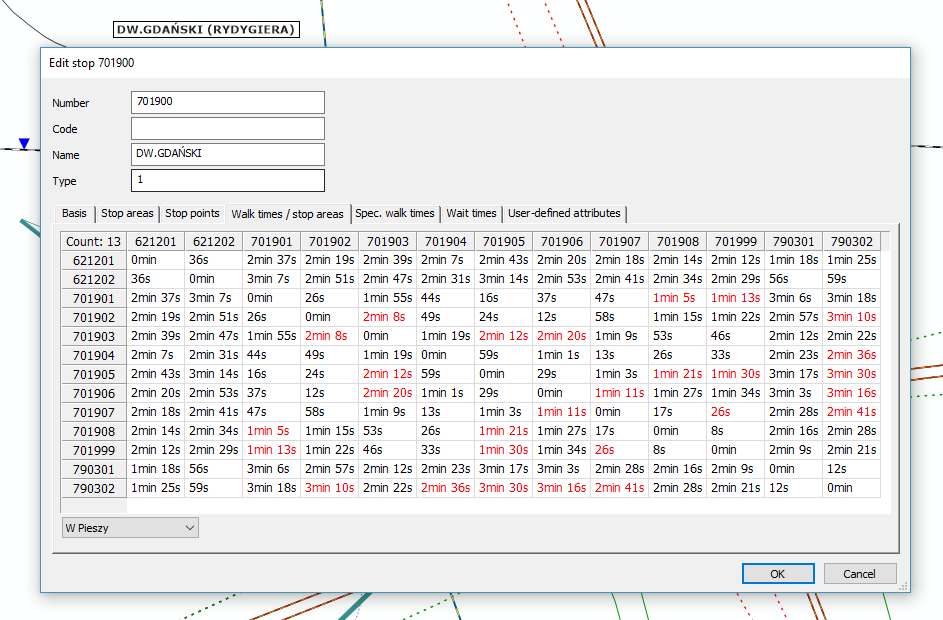
\includegraphics[width=0.9\textwidth]{transfer_times}
 \end{center}  \end{figure} 
\end{frame}

\subsection{Rozkład jazdy}
\begin{frame}{Rozkład jazdy}{Linie zatrzymujące się na przystankach}
\begin{figure}\begin{center}
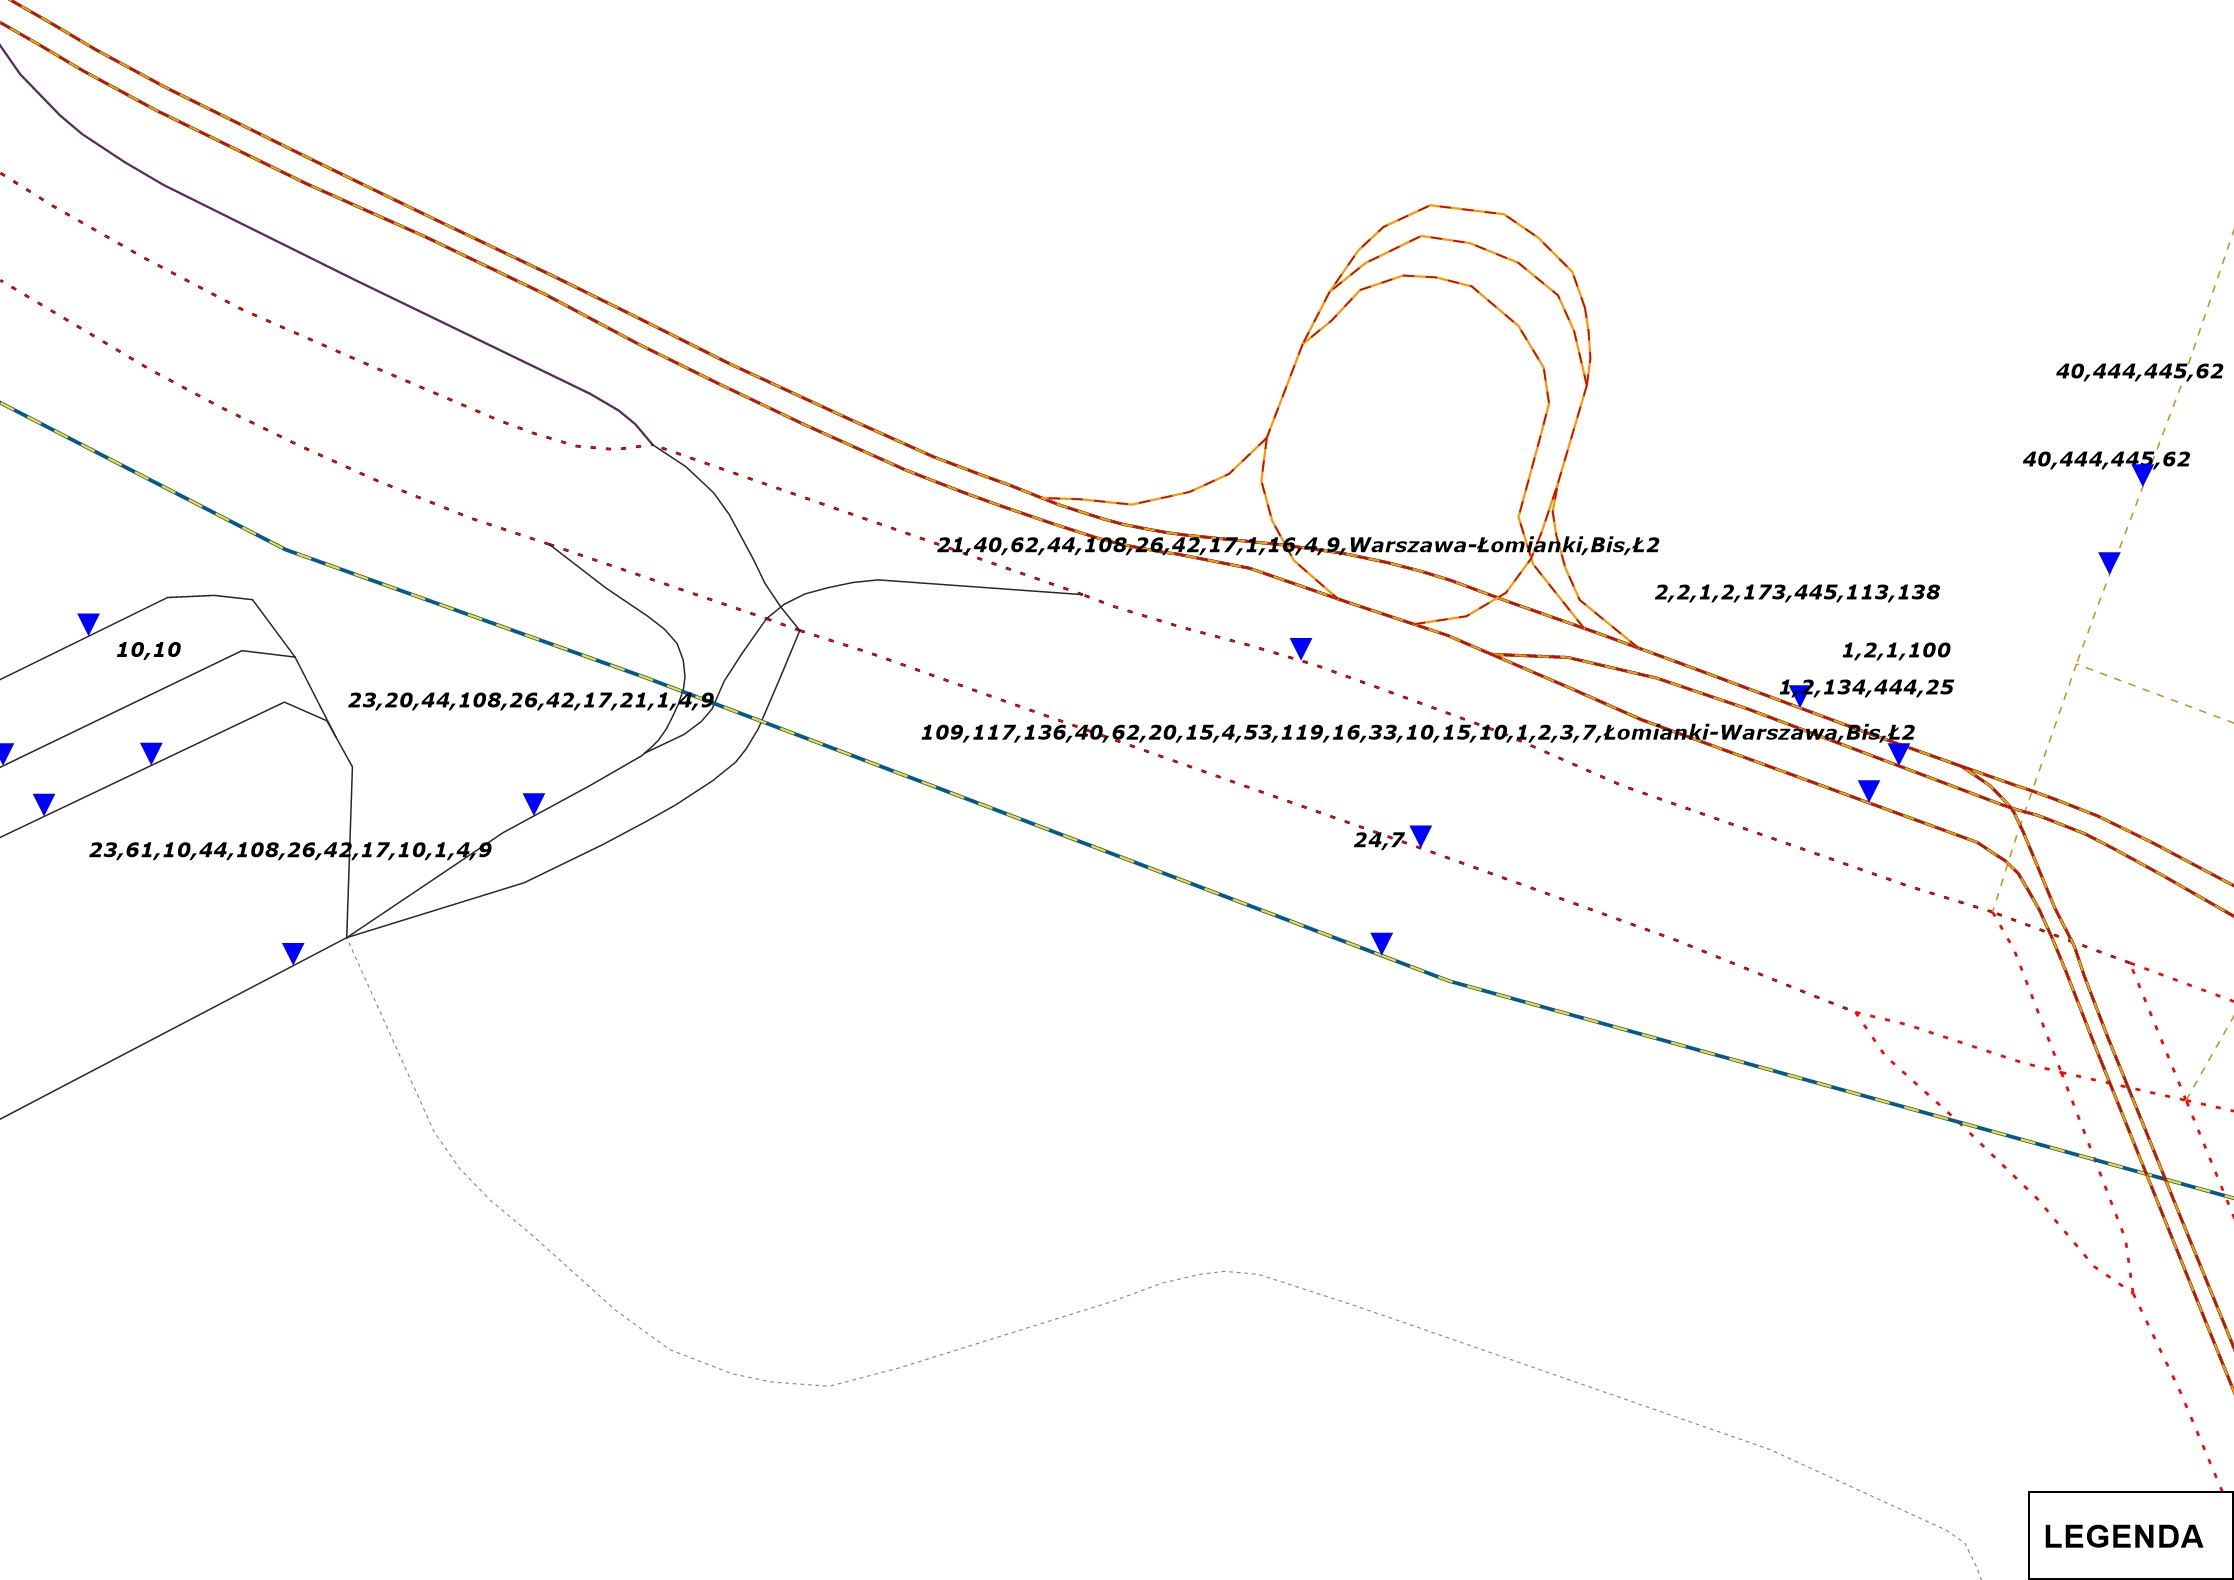
\includegraphics[width=0.9\textwidth]{lines}
 \end{center}  \end{figure} 
\end{frame}

\begin{frame}{Przebieg linii}{autobus}
\begin{figure}\begin{center}
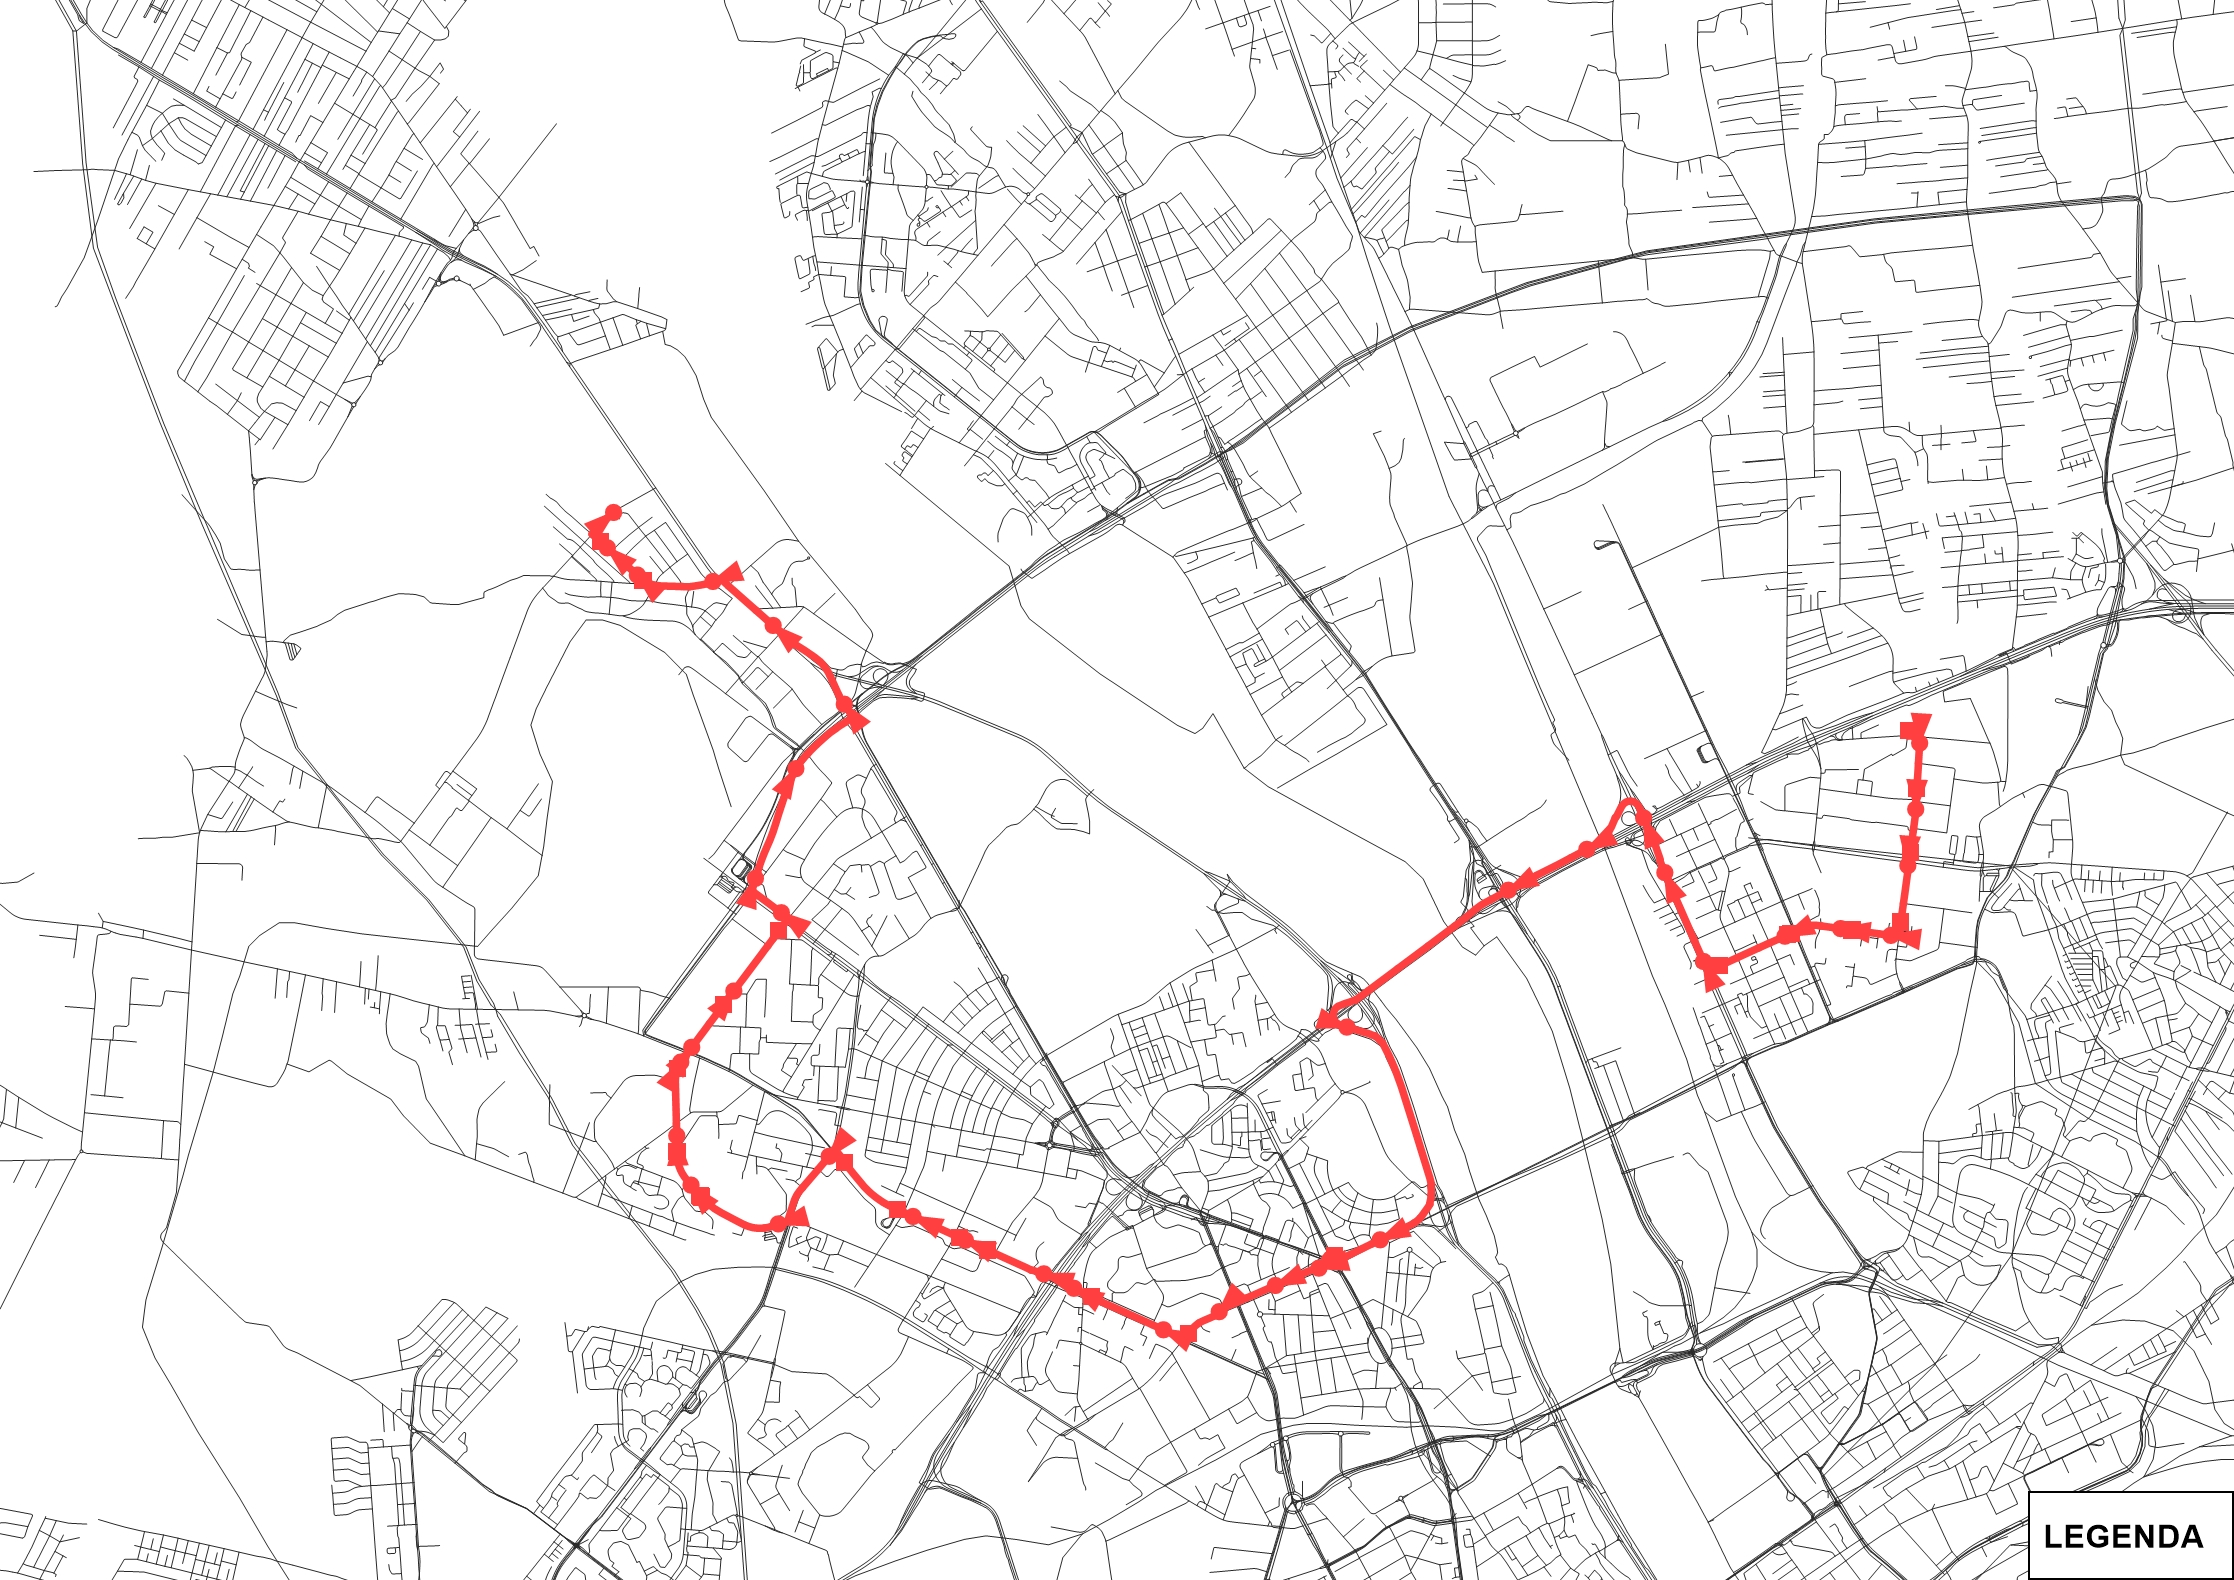
\includegraphics[width=0.9\textwidth]{line}
 \end{center}  \end{figure} 
\end{frame}

\begin{frame}{Przebieg linii}{kolej}
\begin{figure}\begin{center}
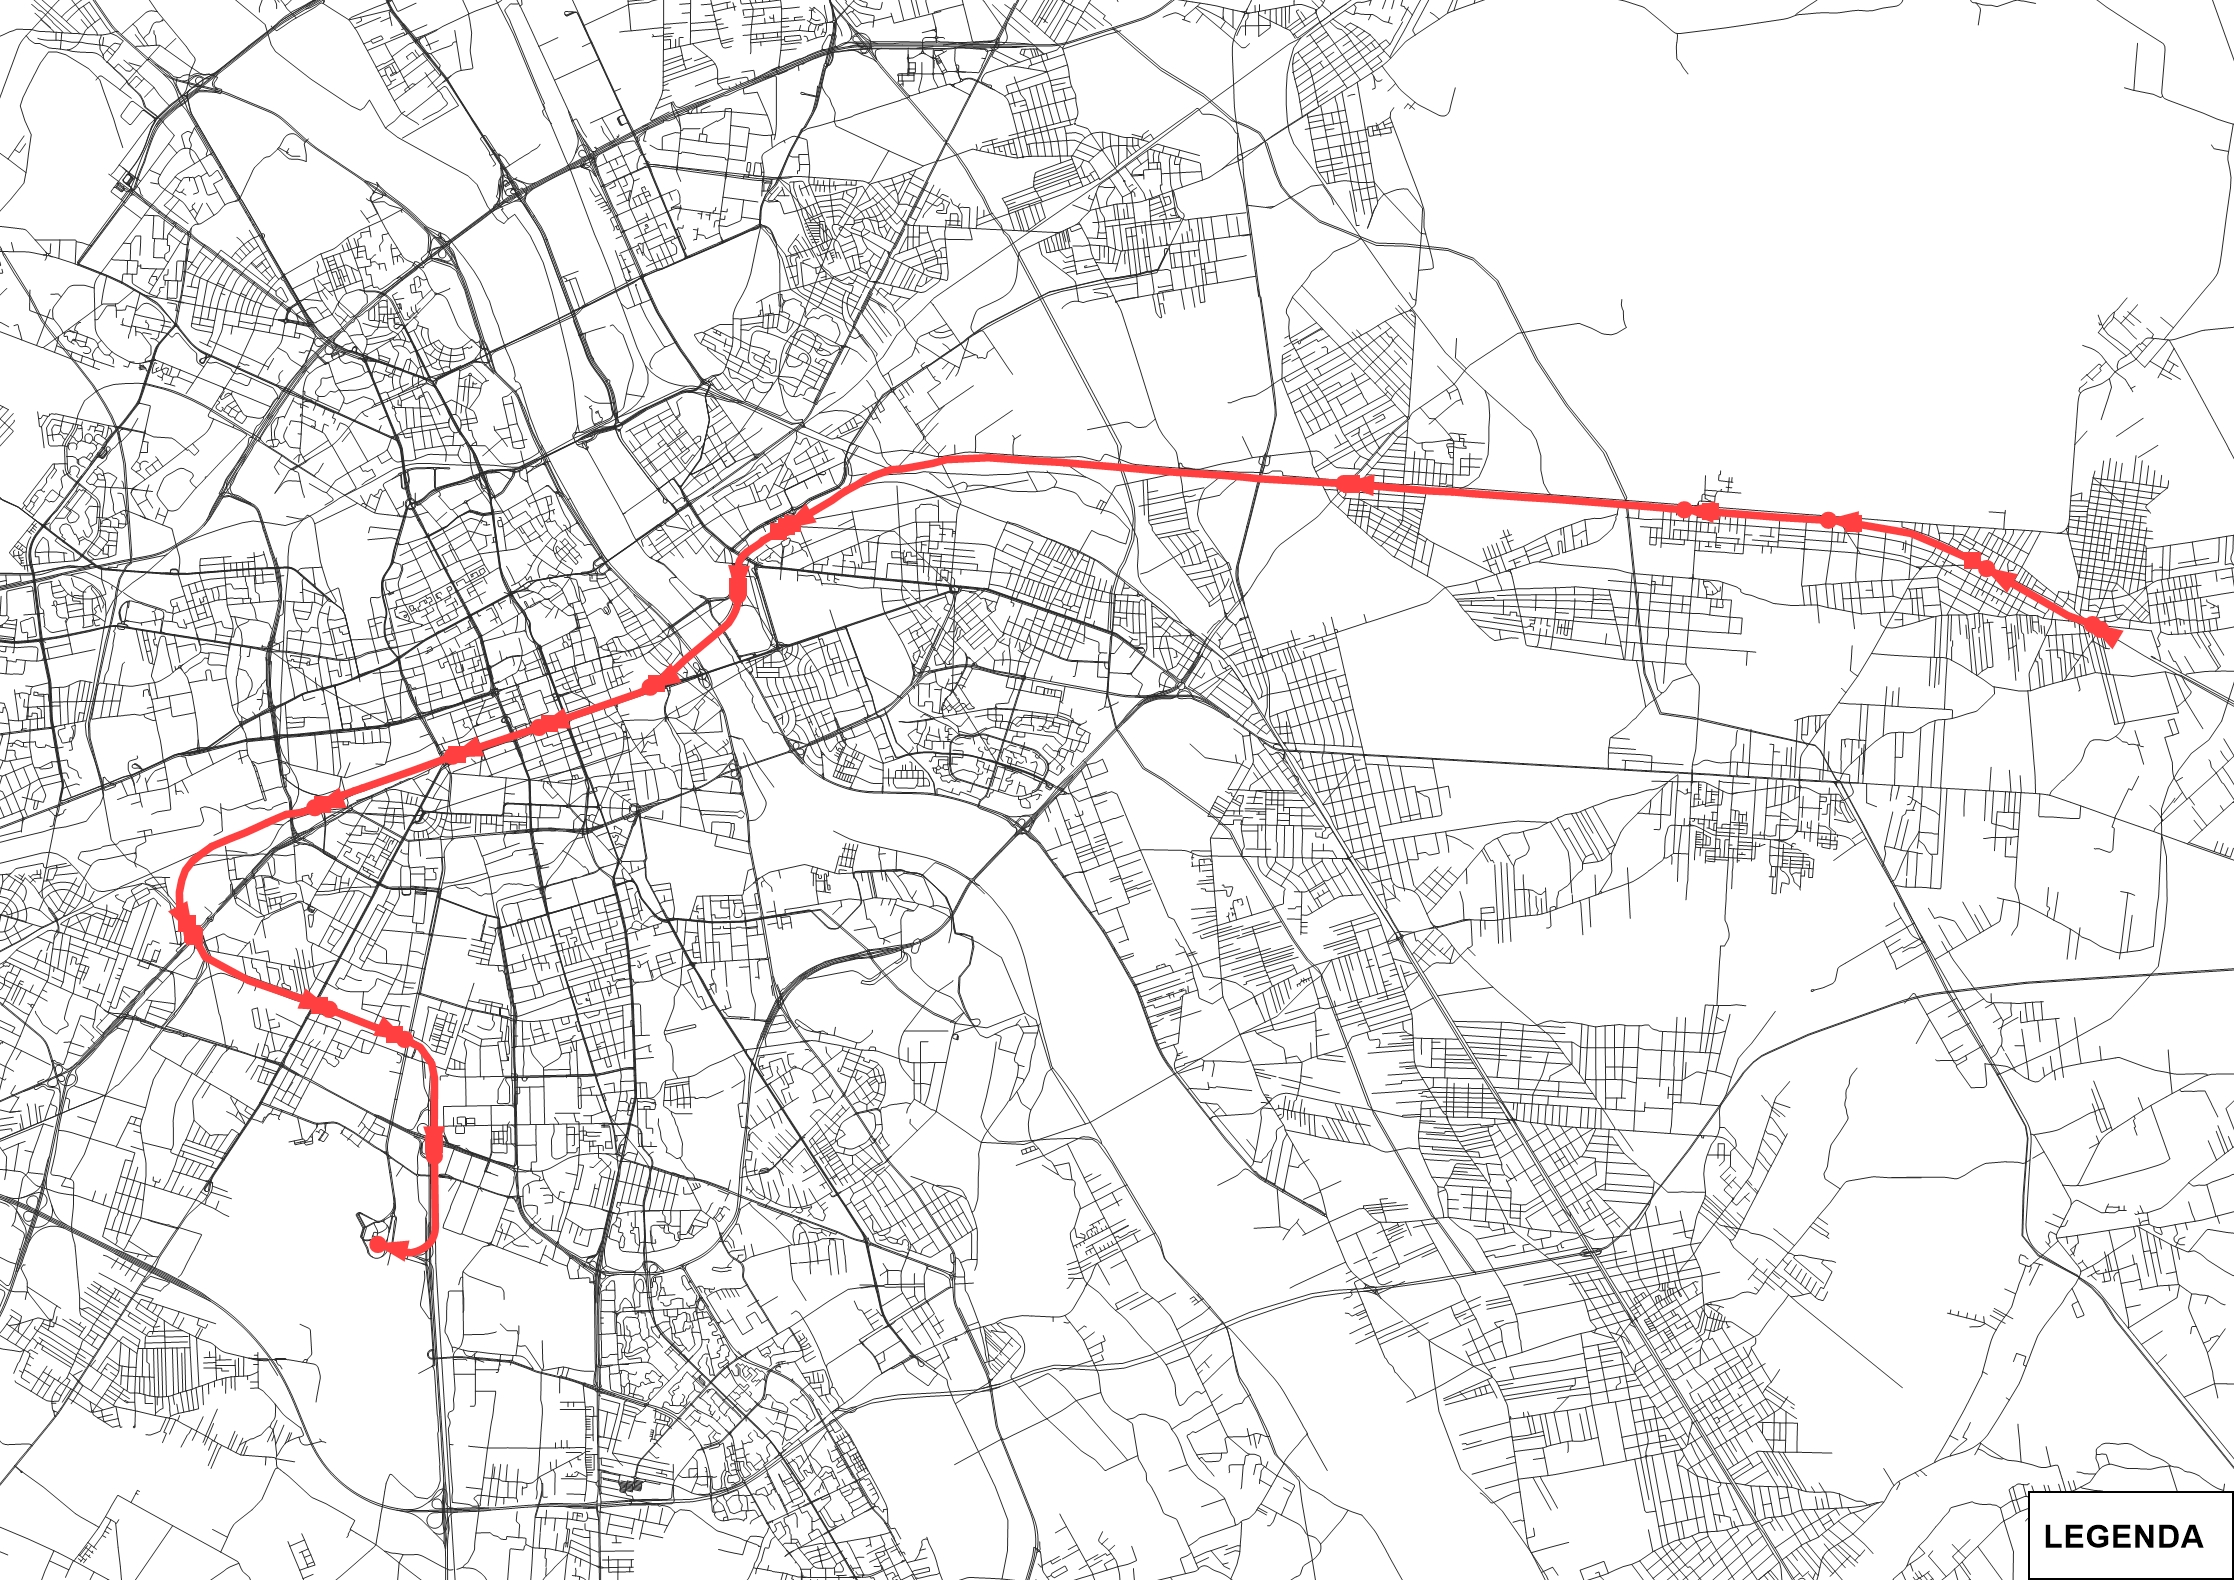
\includegraphics[width=0.9\textwidth]{line2}
 \end{center}  \end{figure} 
\end{frame}

\begin{frame}{Przebieg linii}{wiązka}
\begin{figure}\begin{center}
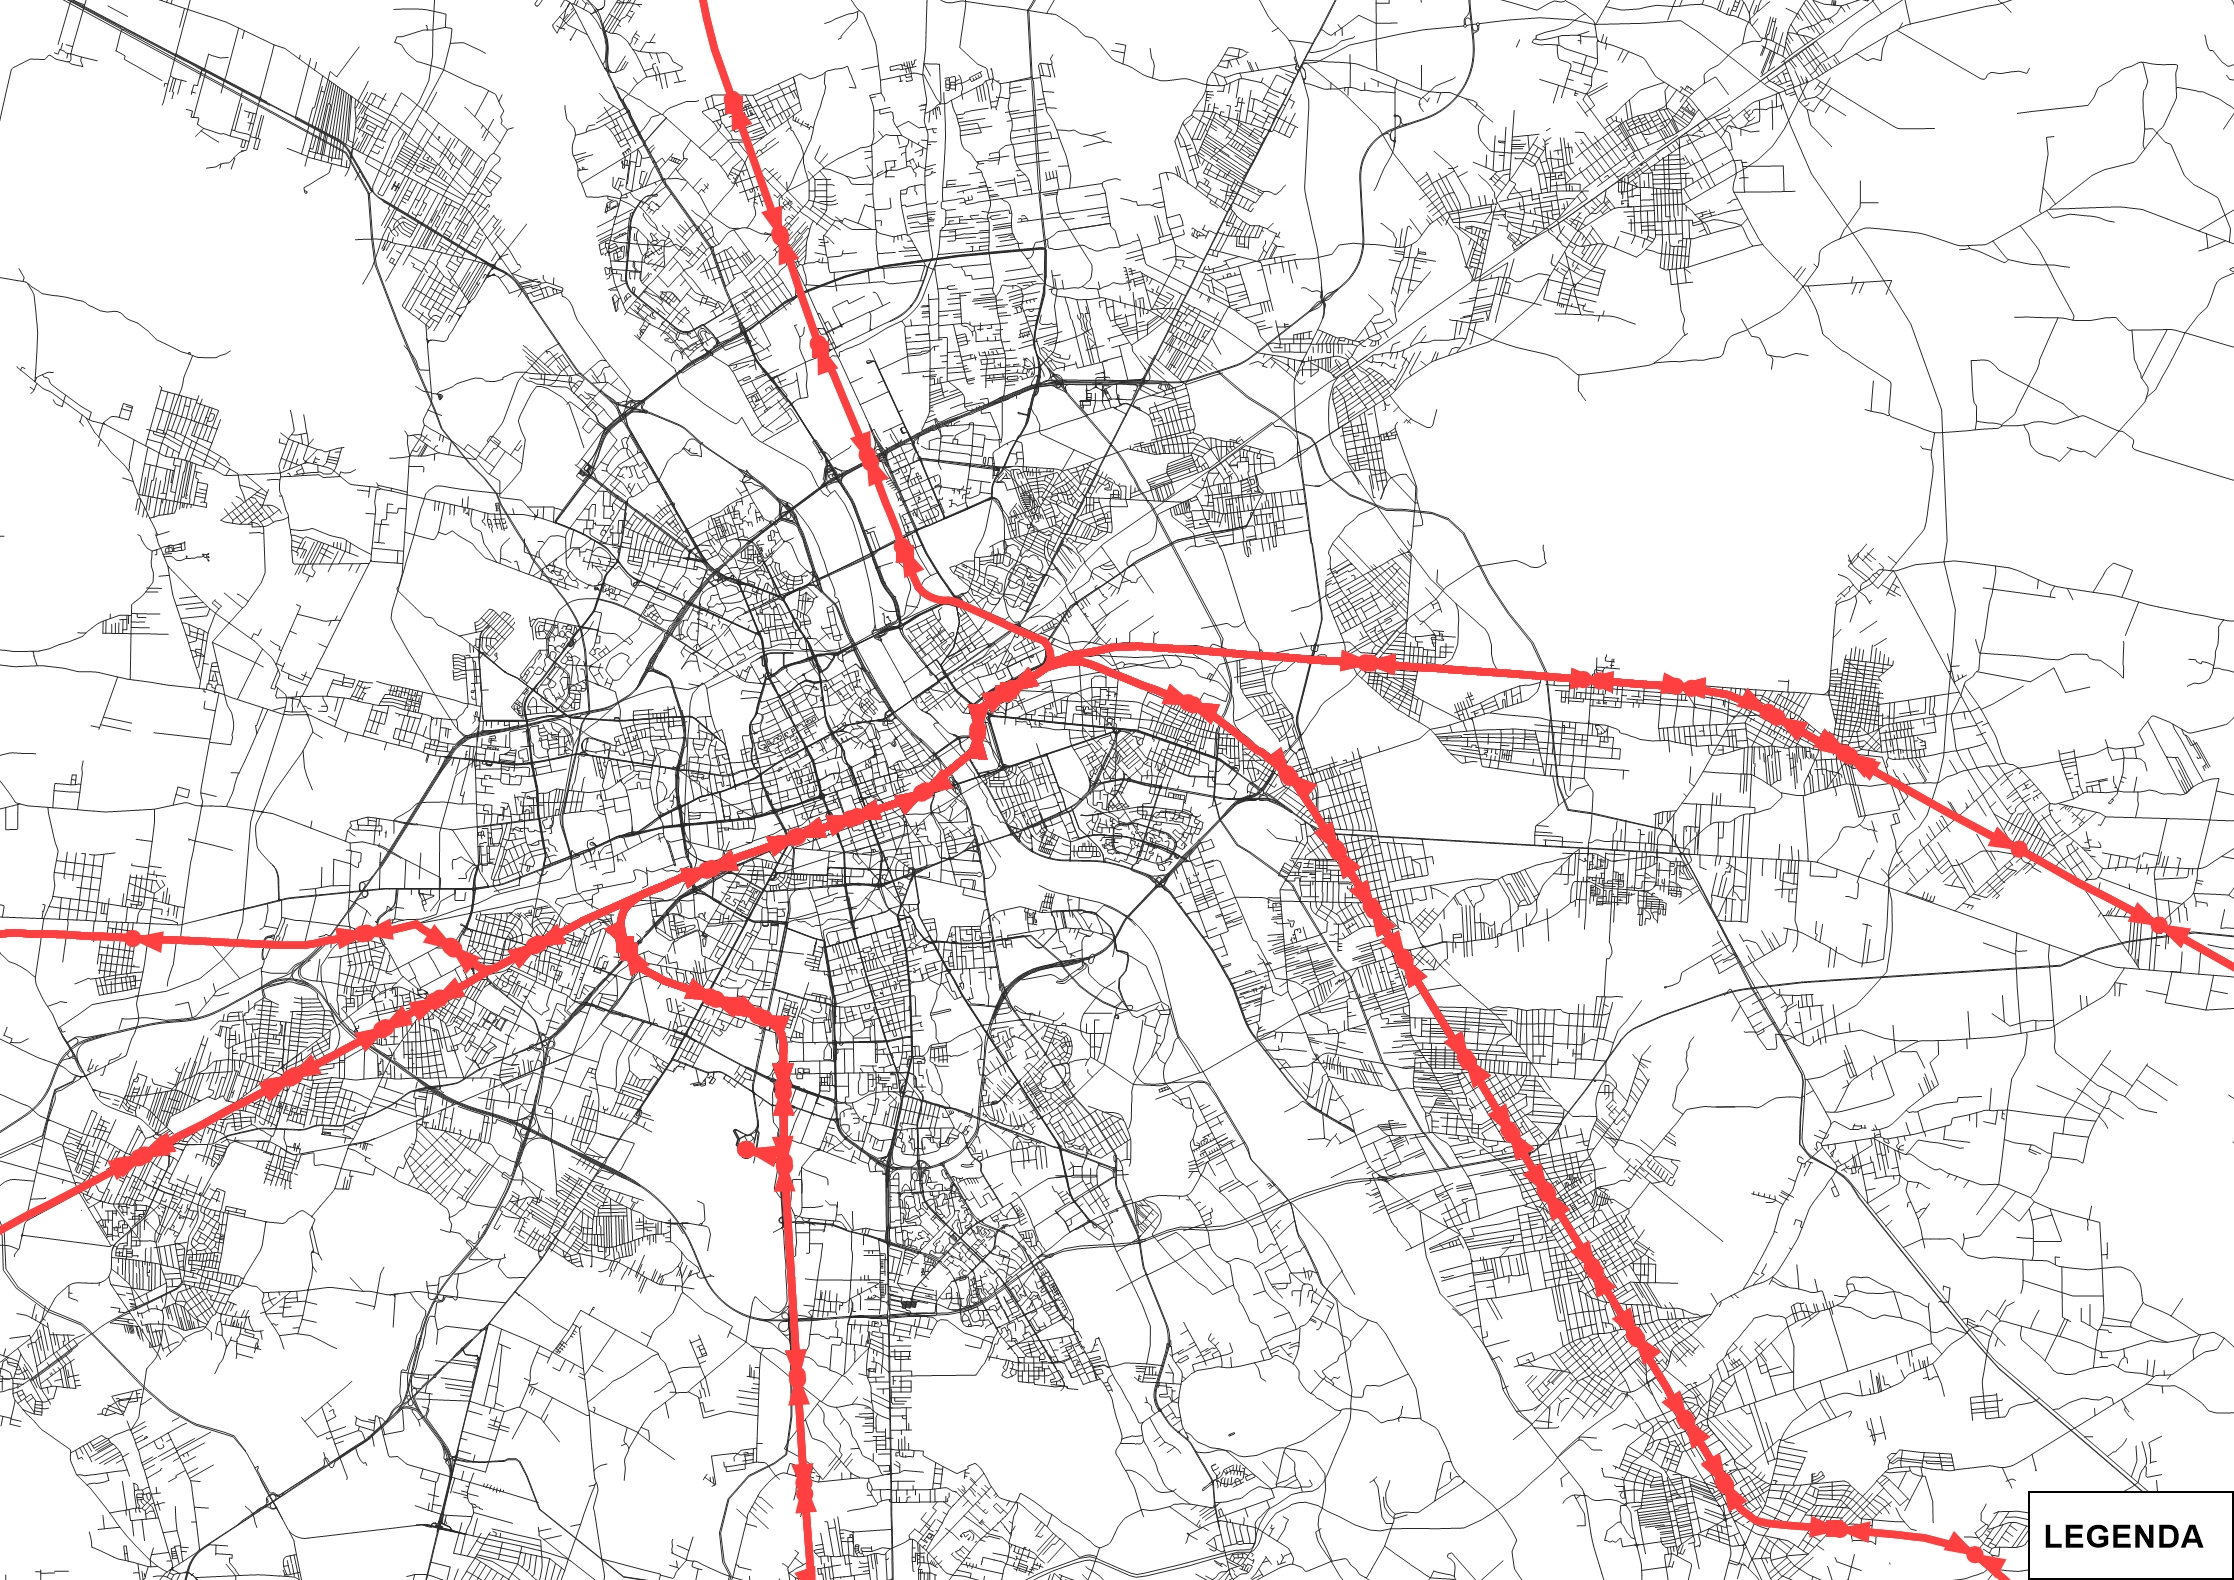
\includegraphics[width=0.9\textwidth]{line3}
 \end{center}  \end{figure} 
\end{frame}

\begin{frame}{Trasa}{sekwencja przystanków i czas rozkładowy}
\begin{figure}\begin{center}
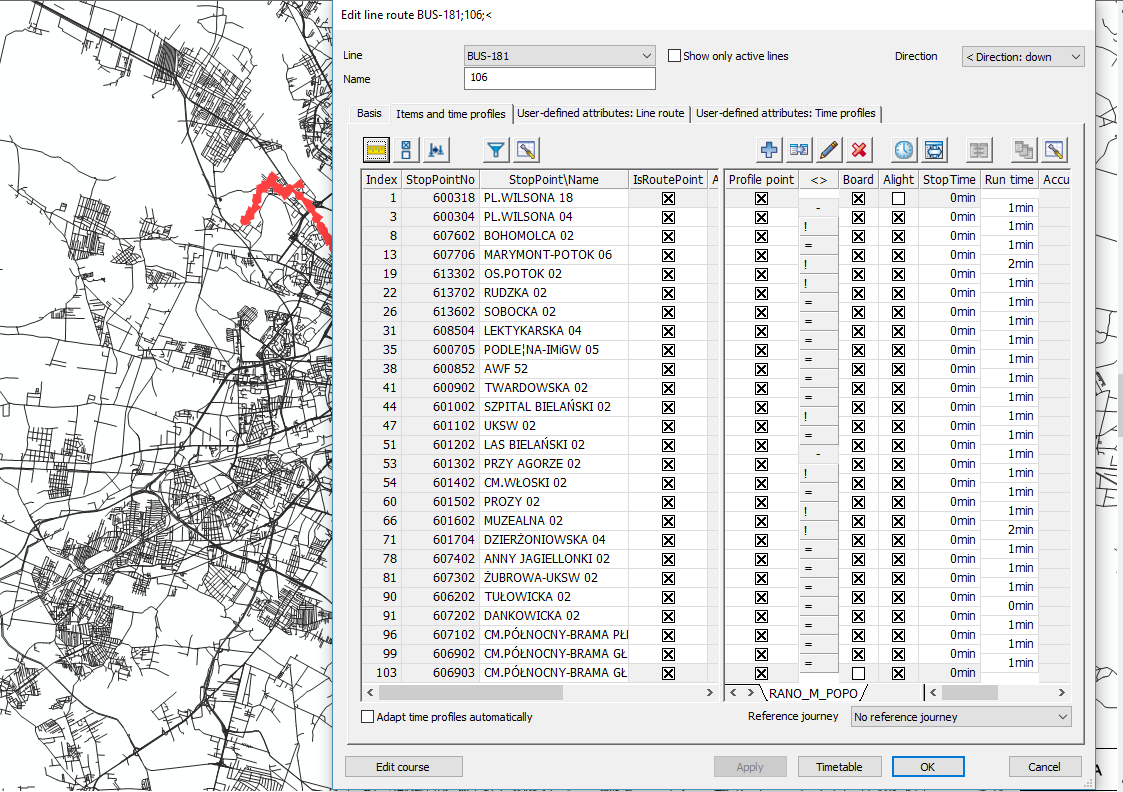
\includegraphics[width=0.9\textwidth]{route}
 \end{center}  \end{figure} 
\end{frame}

\begin{frame}{Trasa}{rozkład jazdy}
\begin{figure}\begin{center}
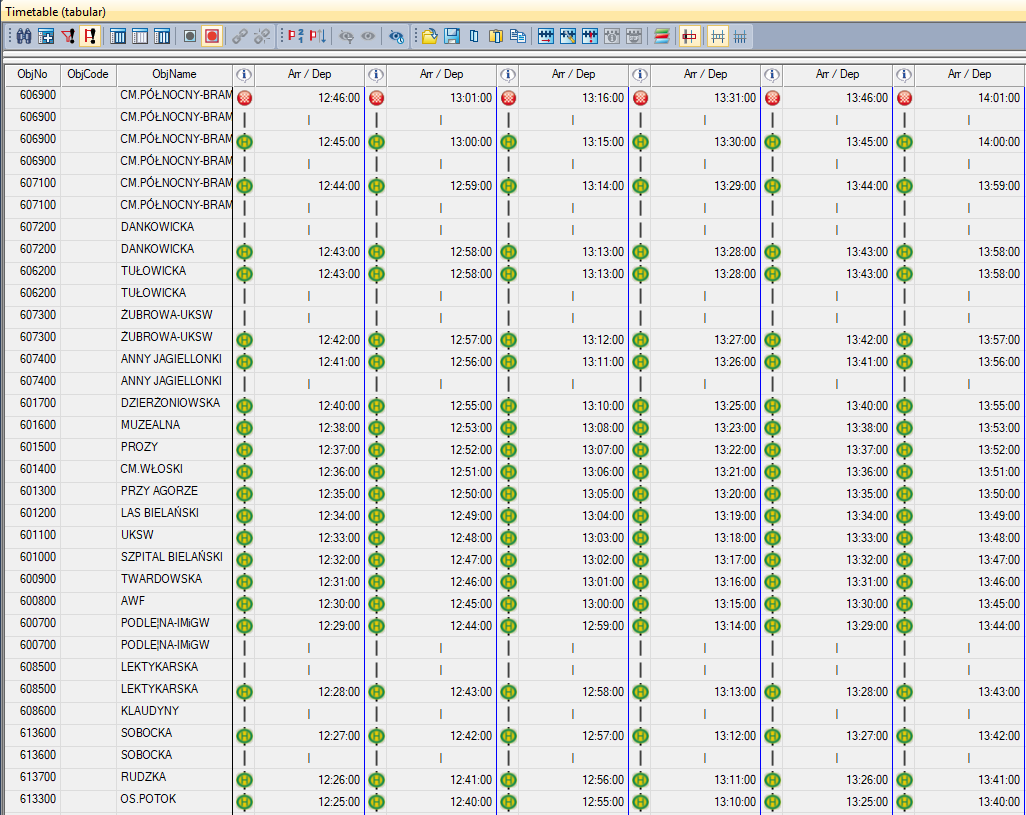
\includegraphics[width=0.9\textwidth]{timetable1}
 \end{center}  \end{figure} 
\end{frame}


\section{Warstwy dodatkowe}
\begin{frame}{Warstwy SIP}{Oznakowanie pionowe (znaki)}
\begin{figure}\begin{center}
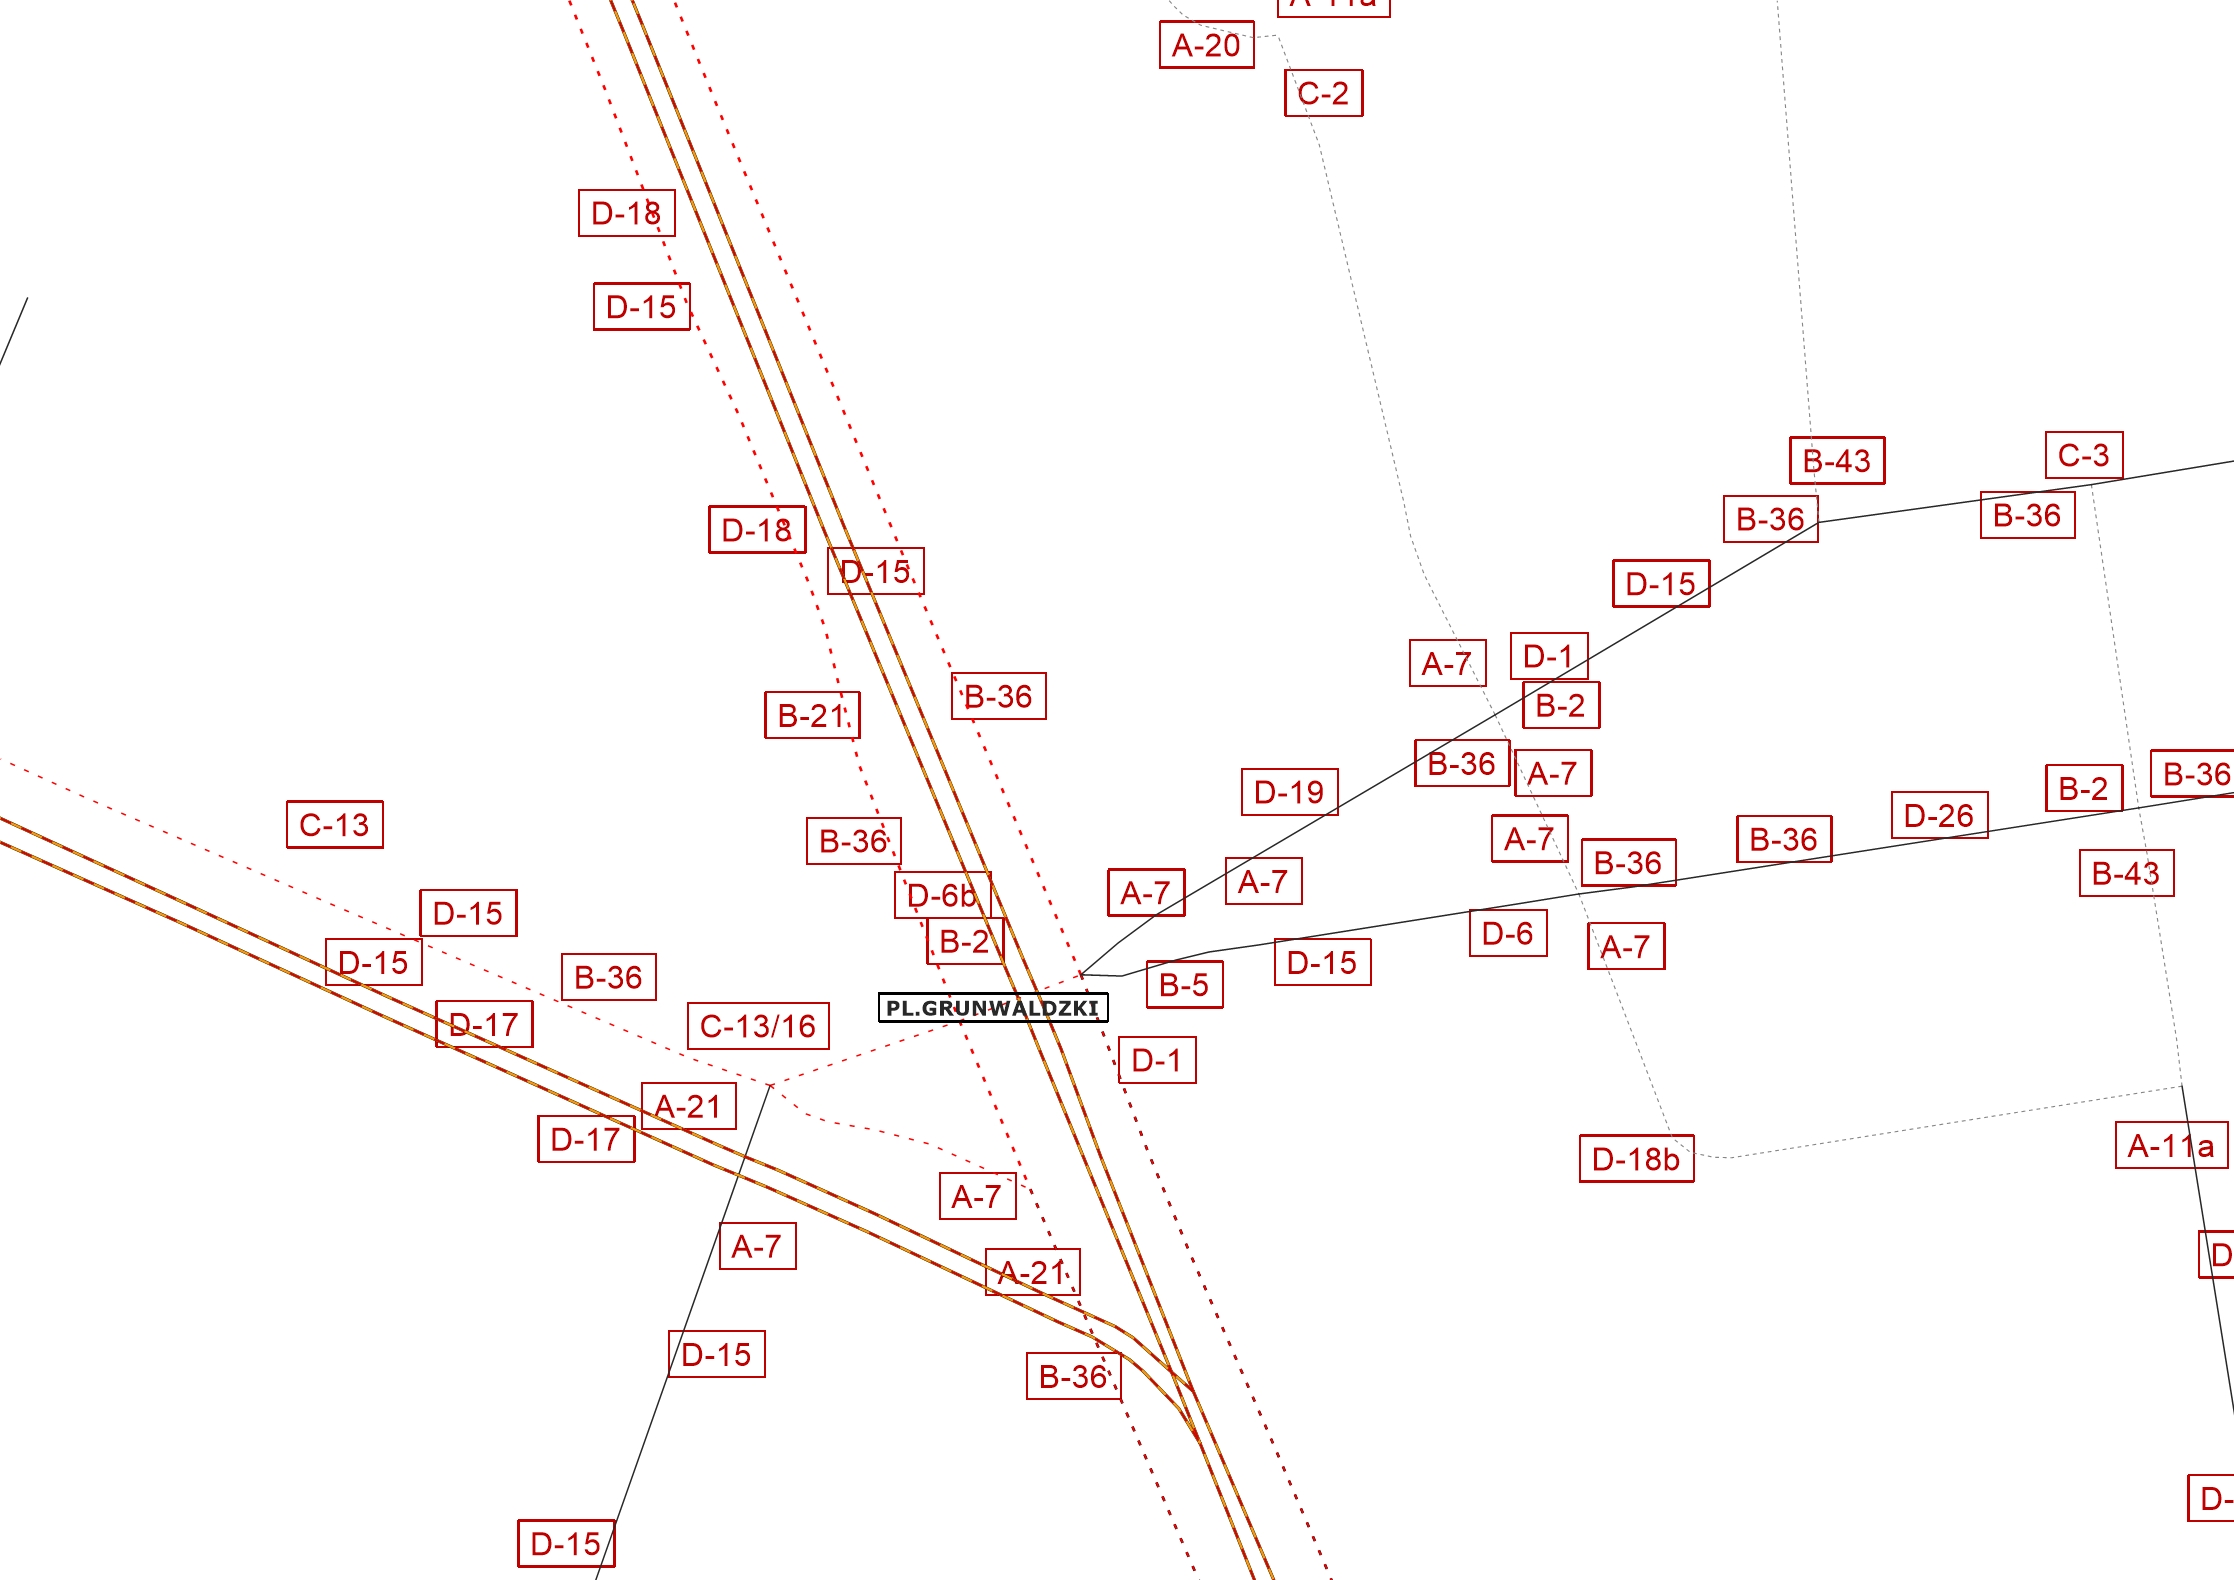
\includegraphics[width=0.9\textwidth]{POI1}
 \end{center}  \end{figure} 
\end{frame}

\begin{frame}{Warstwy SIP}{Oznakowanie poziomie (strzałki)}
\begin{figure}\begin{center}
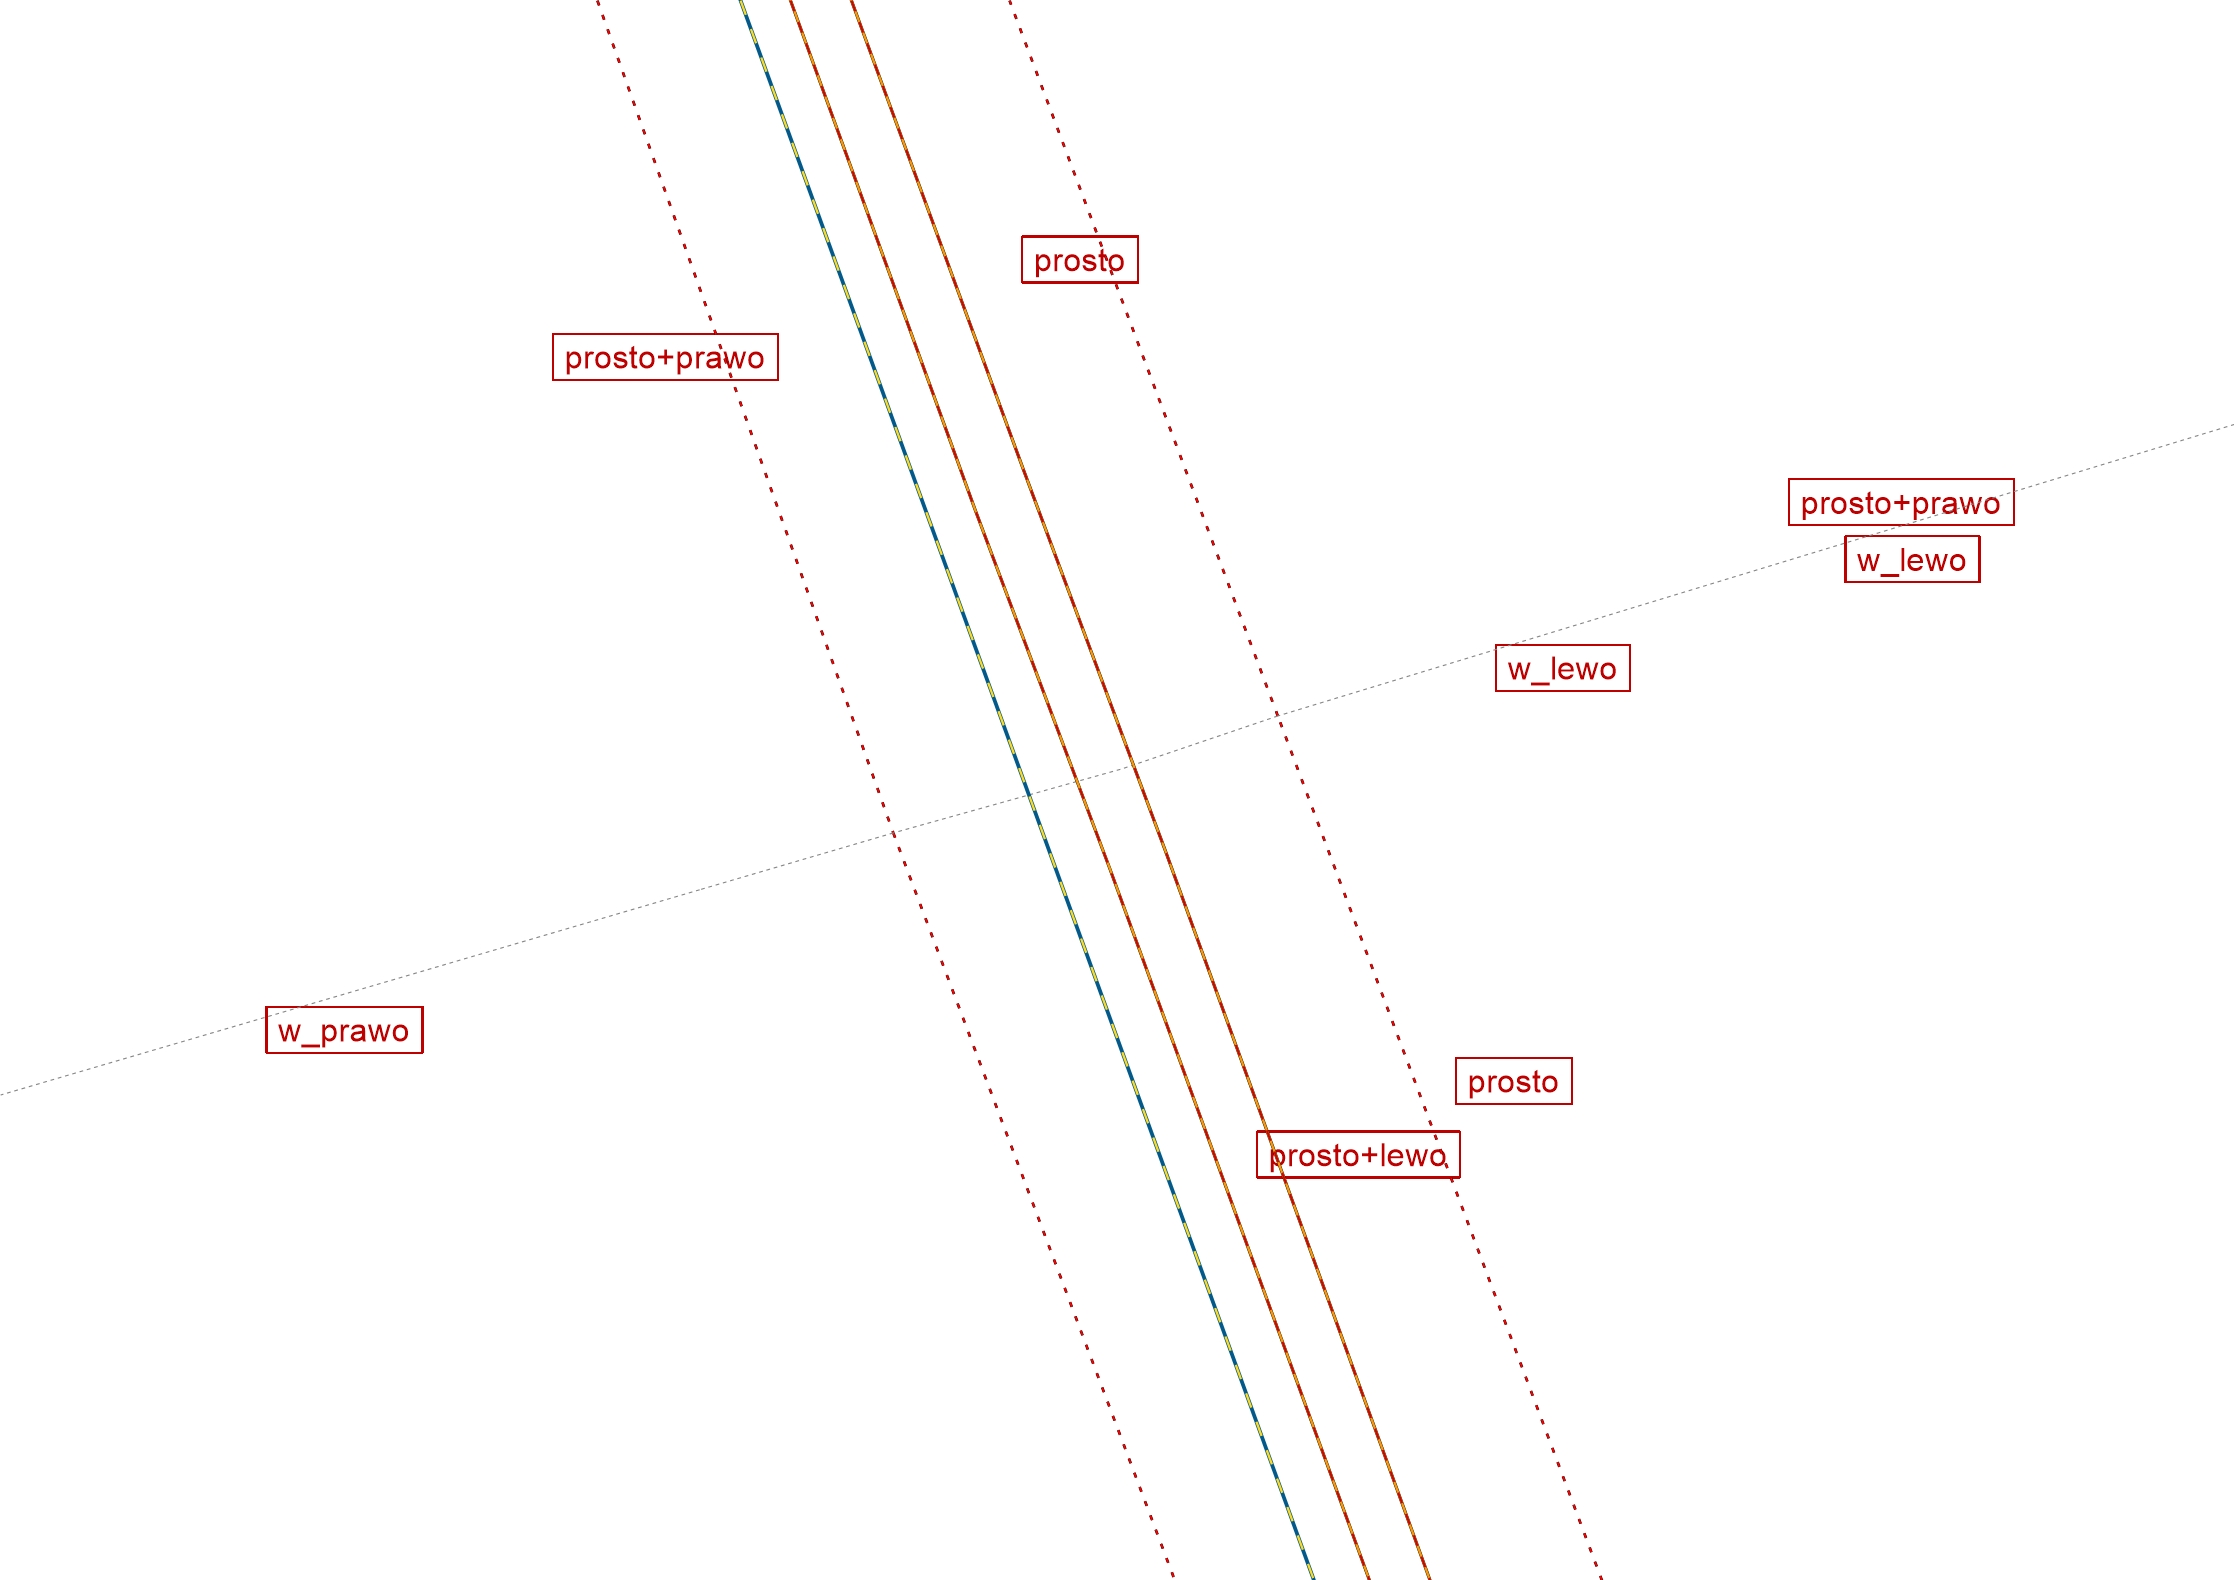
\includegraphics[width=0.9\textwidth]{strzalki}
 \end{center}  \end{figure} 
\end{frame}

\begin{frame}{Warstwy SIP}{Parkingi}
\begin{figure}\begin{center}
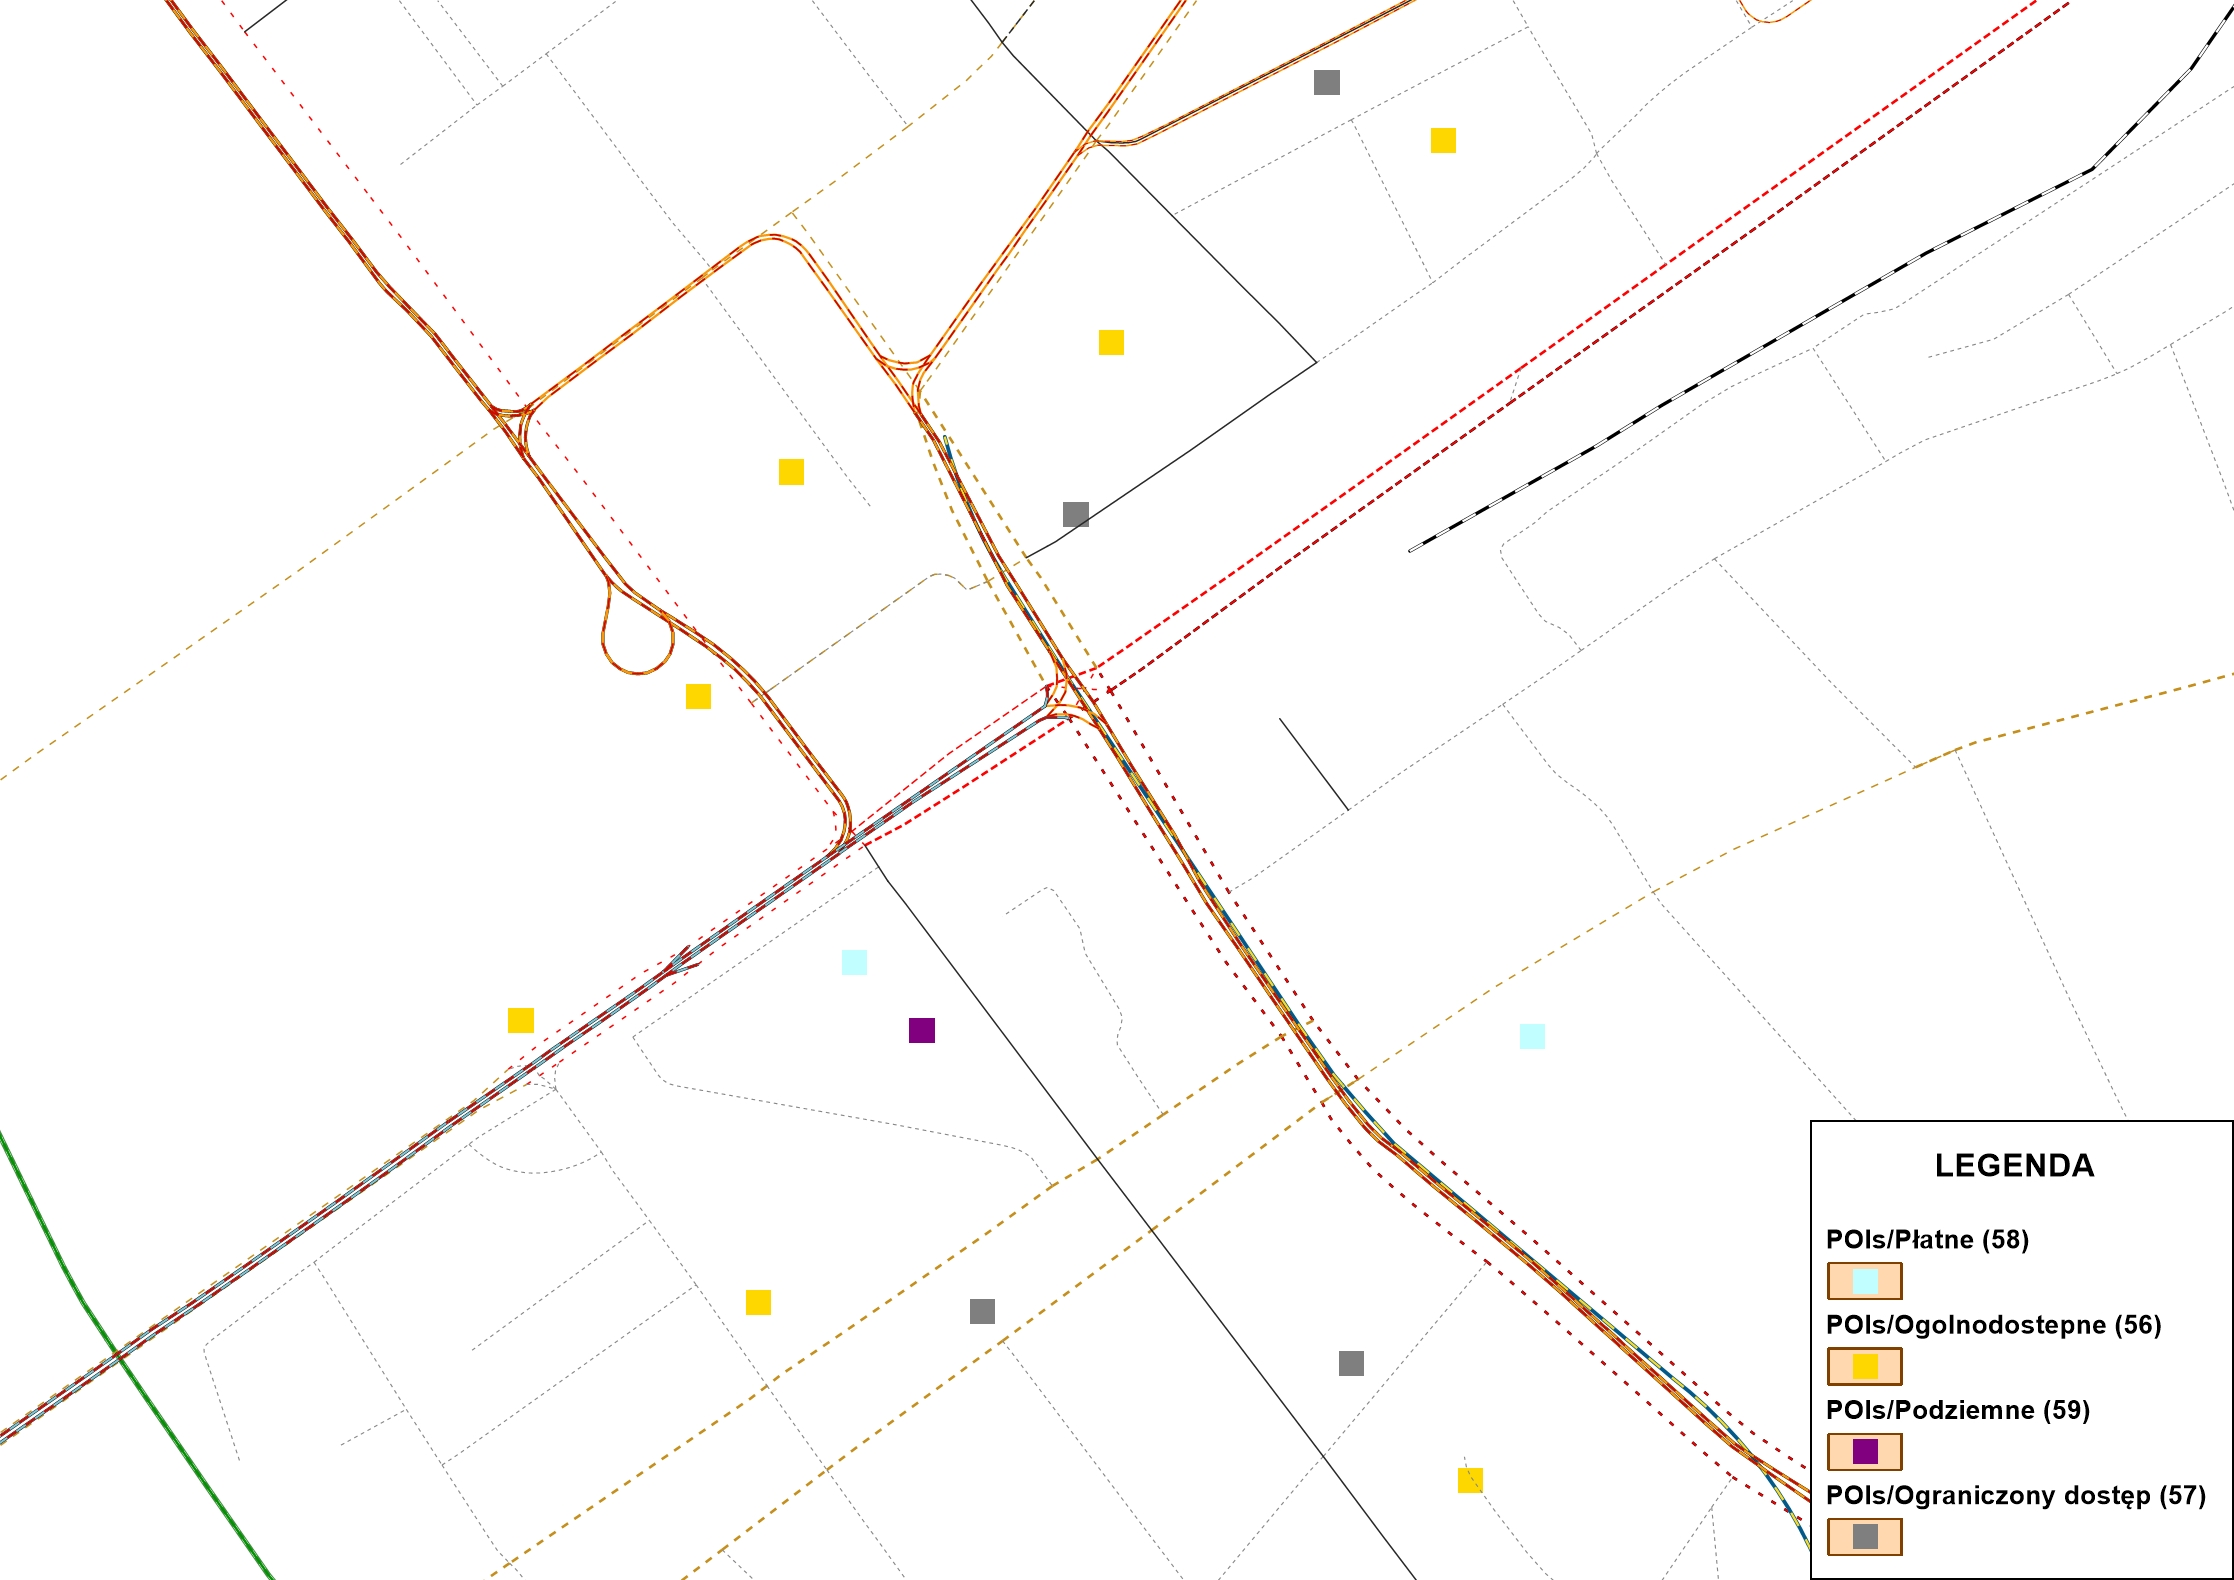
\includegraphics[width=0.9\textwidth]{parking}
 \end{center}  \end{figure} 
\end{frame}

\begin{frame}{Warstwy SIP}{Stacje roweru miejskiego}
\begin{figure}\begin{center}
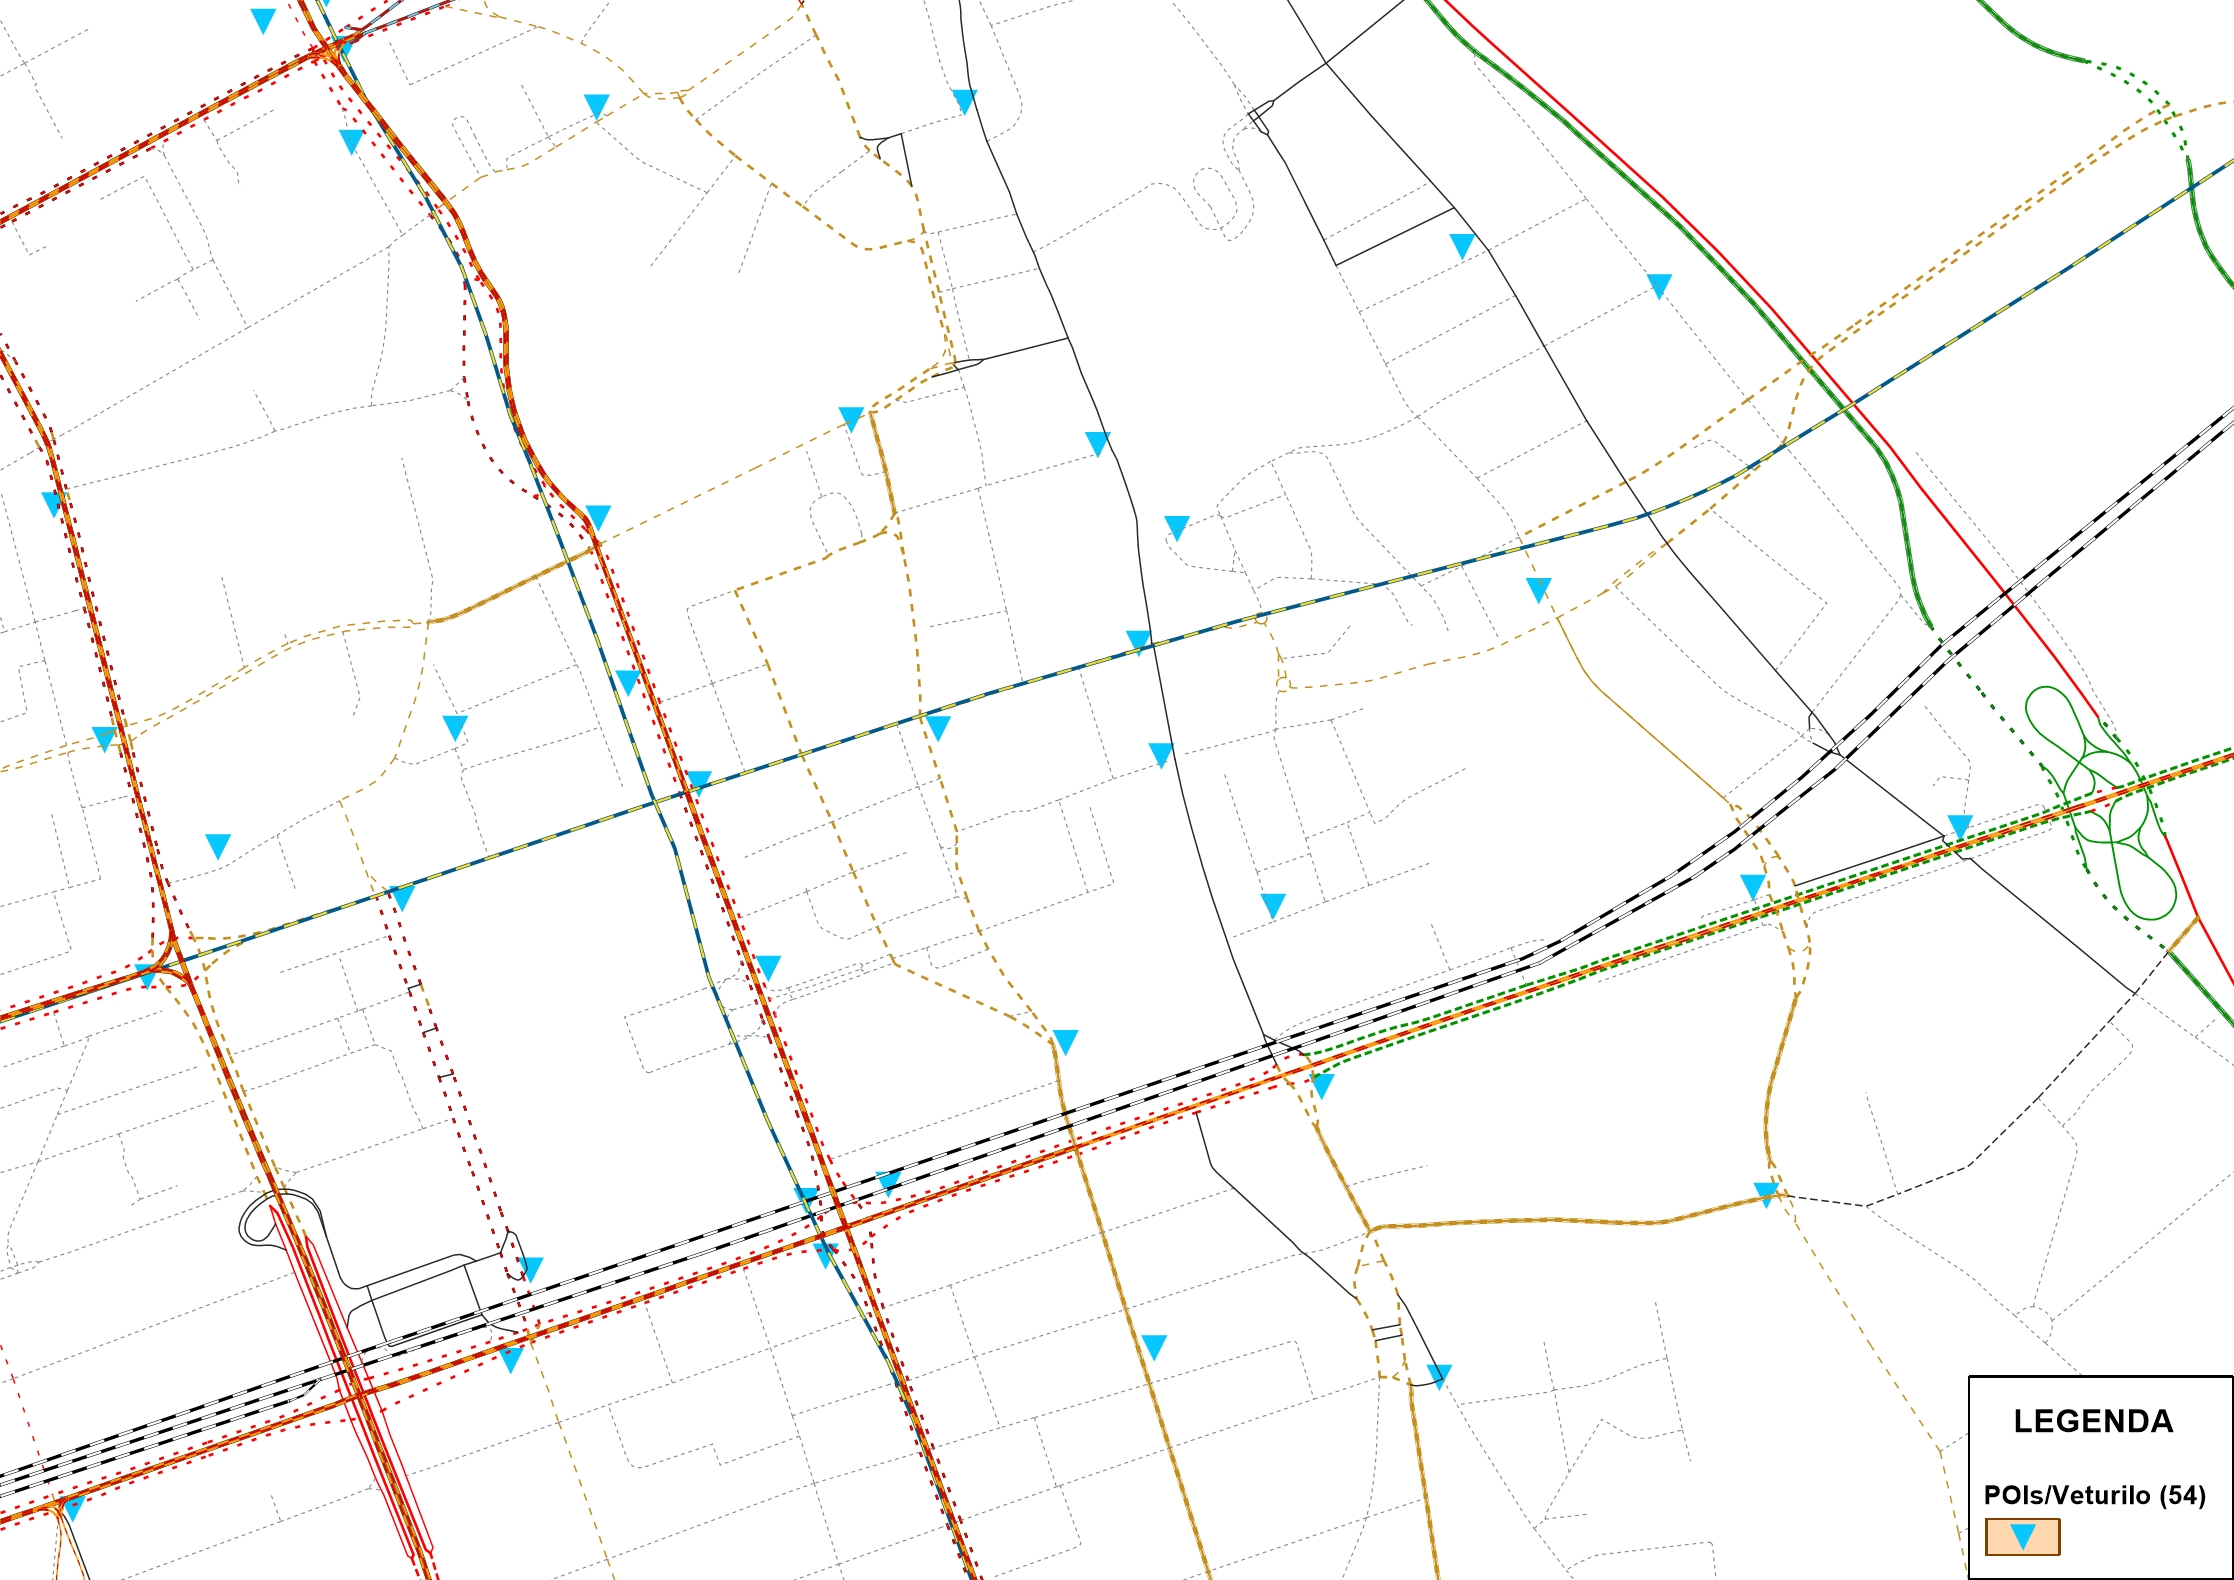
\includegraphics[width=0.9\textwidth]{bike}
 \end{center}  \end{figure} 
\end{frame}

\section{Parametryzacja}
\subsection{Parametryzacja sieci}
\begin{frame}{Odcinek}{podstawowe parametry}
\begin{figure}\begin{center}
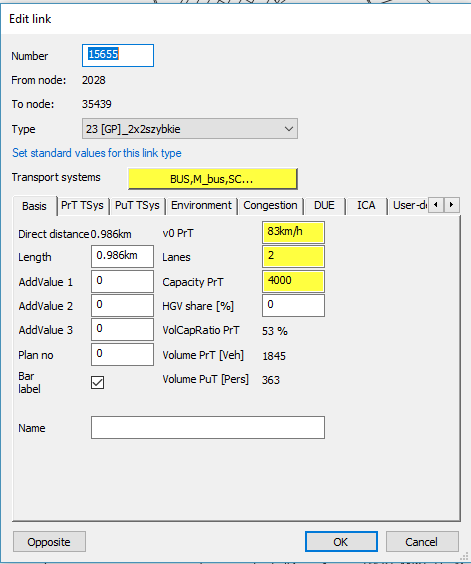
\includegraphics[width=0.5\textwidth]{link}
 \end{center}  \end{figure} 
\end{frame}


\begin{frame}{Odcinek}{dodatkowe parametry (Used Defined Attributes)}
\begin{figure}\begin{center}
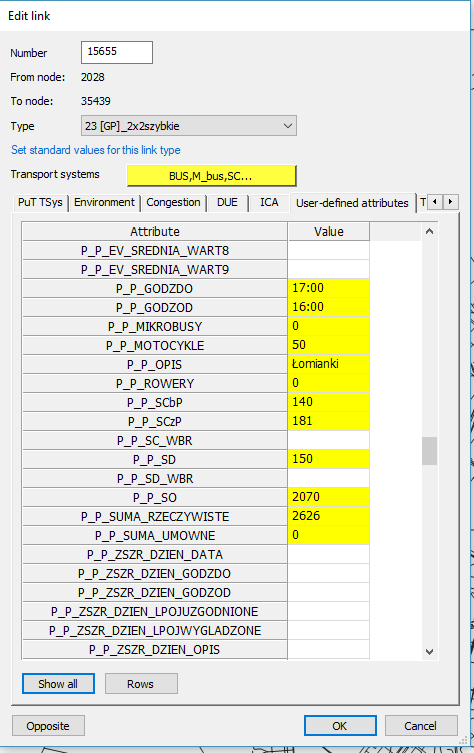
\includegraphics[width=0.4\textwidth]{link2}
 \end{center}  \end{figure} 
\end{frame}

\begin{frame}{Typy odcinków}{parametry}
\begin{figure}\begin{center}
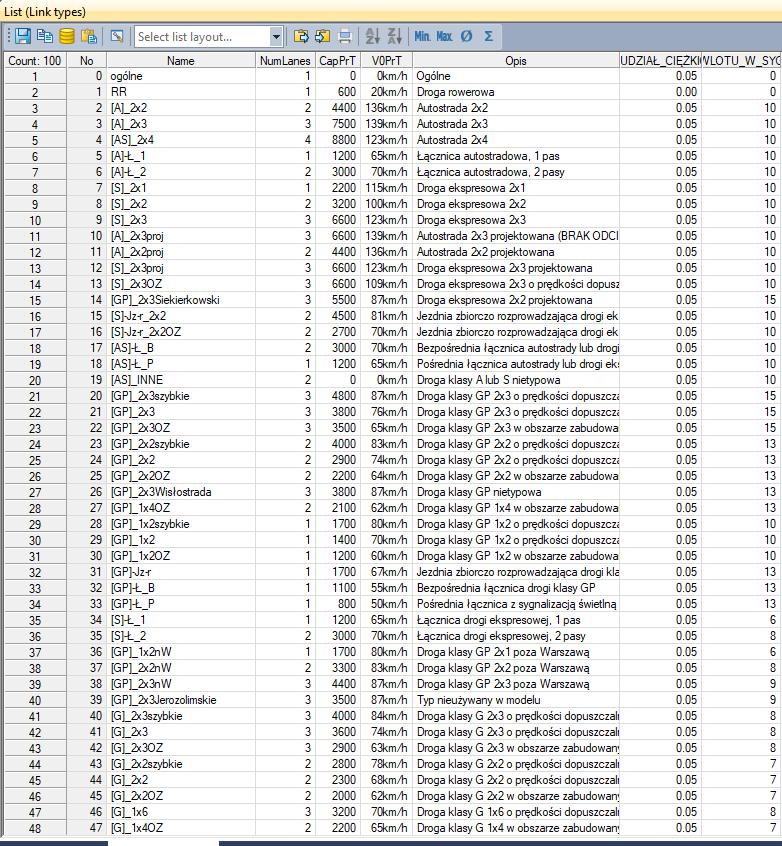
\includegraphics[width=0.8\textwidth]{link_types}
 \end{center}  \end{figure} 
\end{frame}

\begin{frame}{Parametryzacja}{prędkość}
\begin{figure}\begin{center}
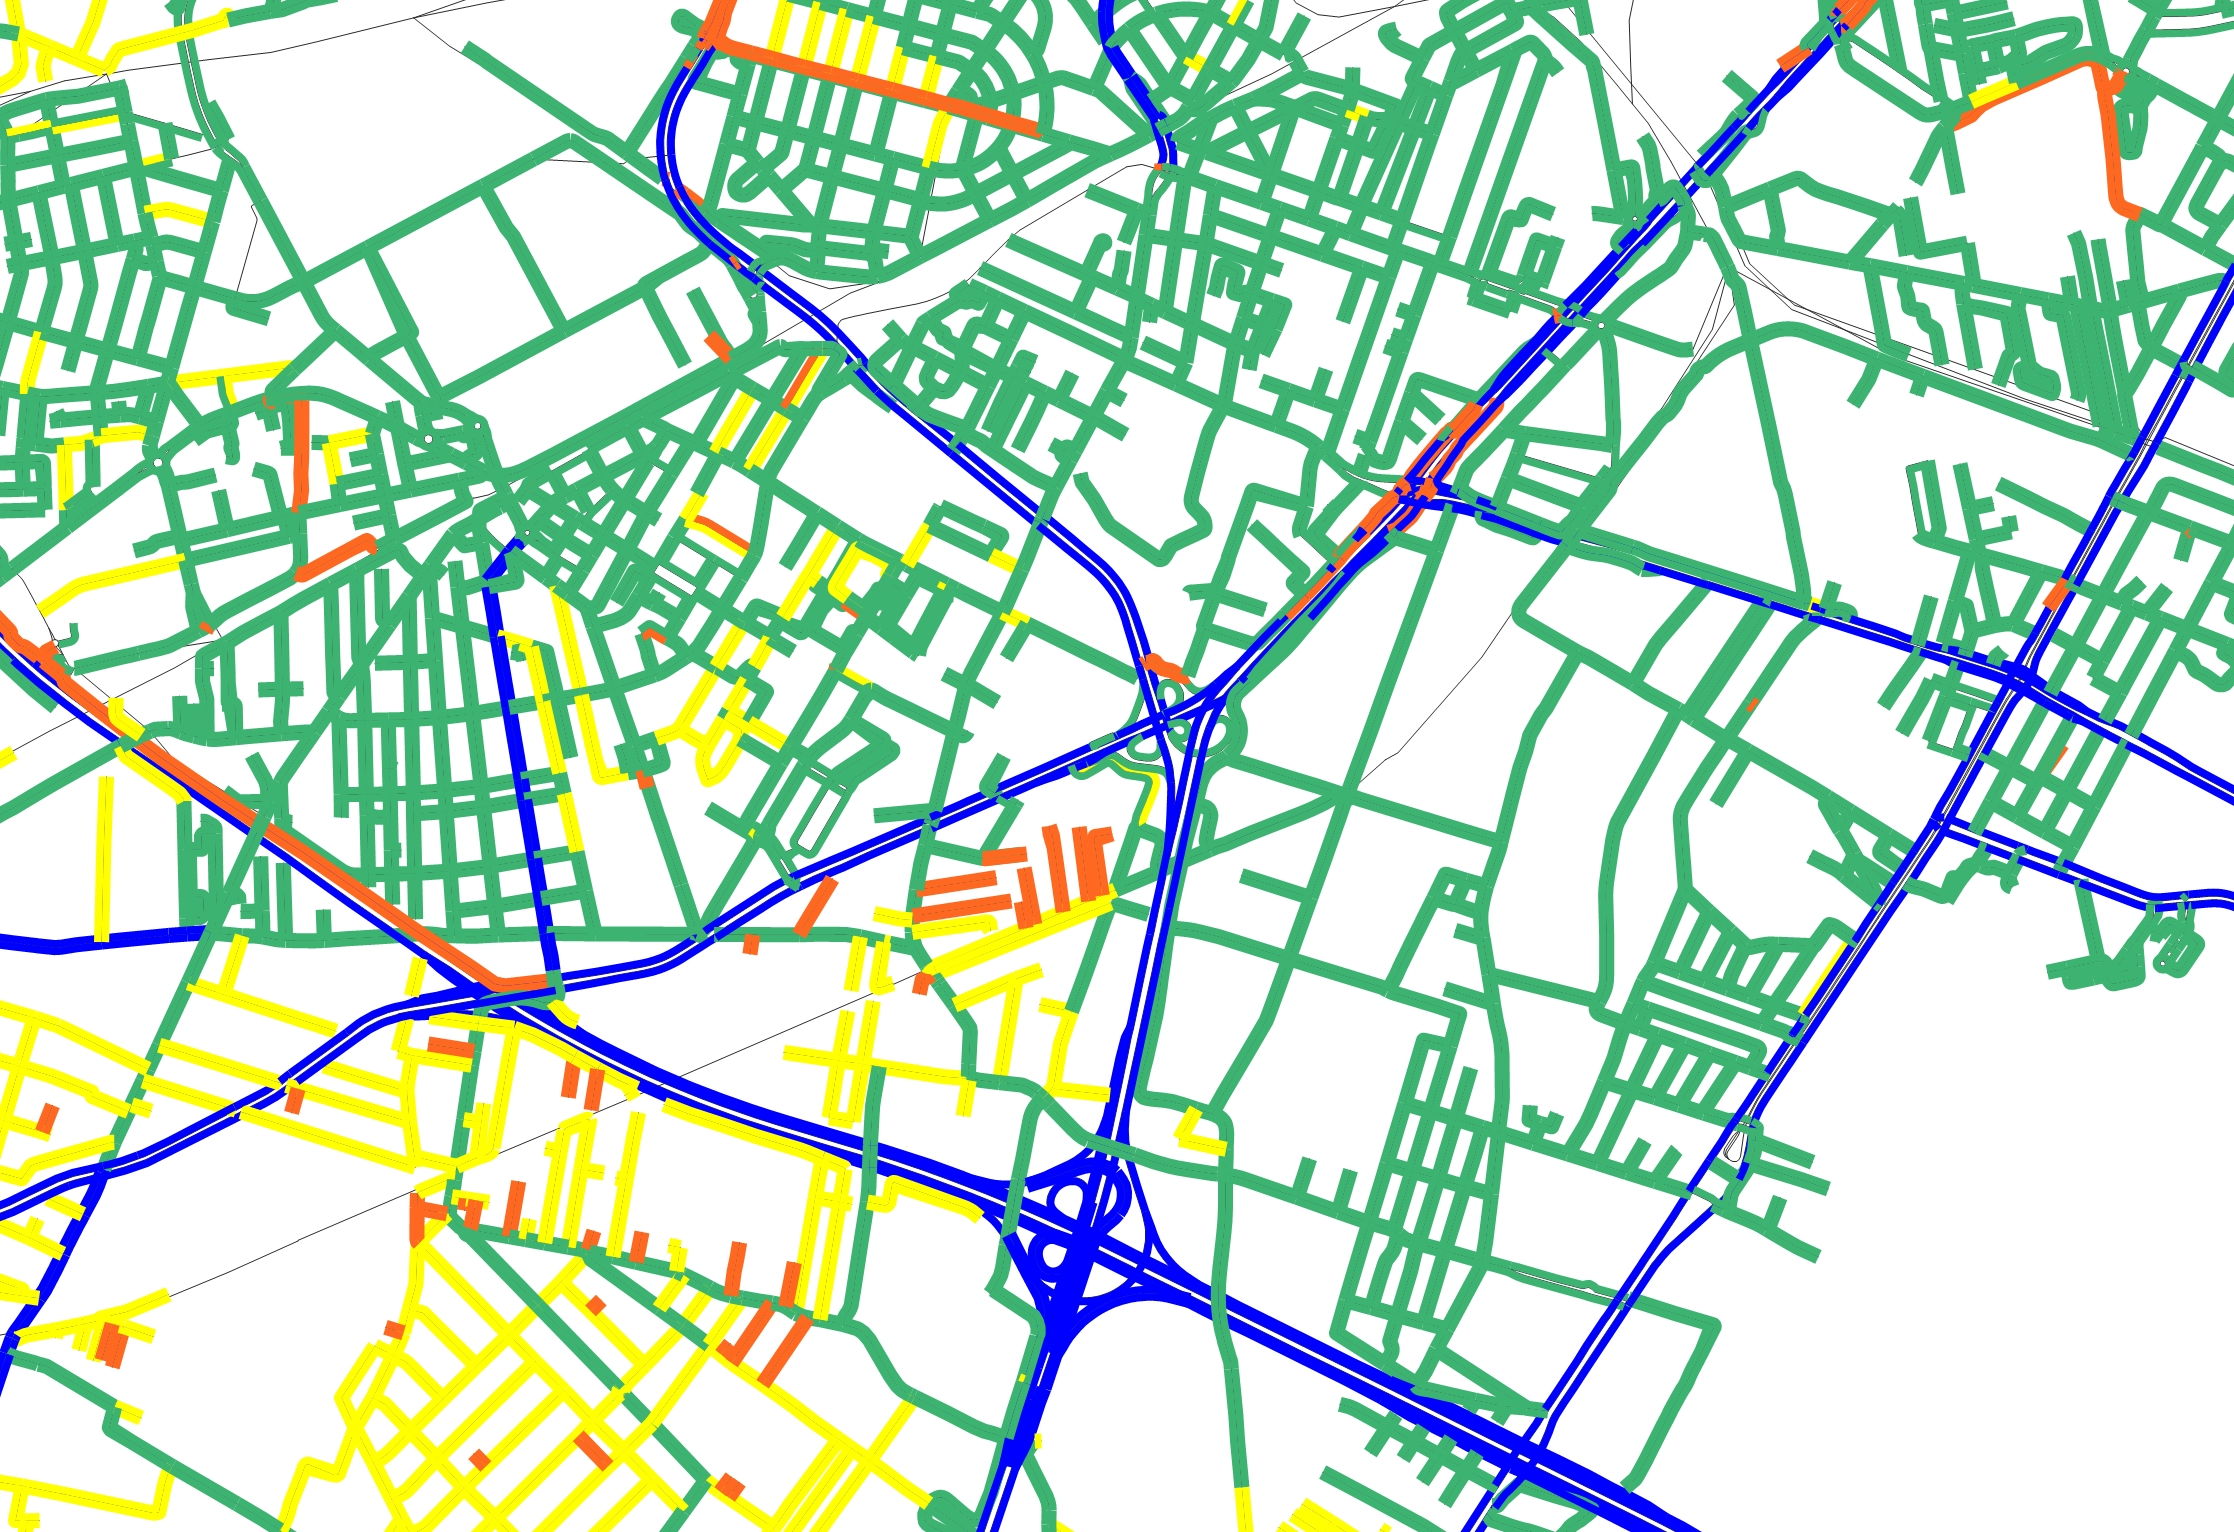
\includegraphics[width=0.8\textwidth]{speed_map}
 \end{center}  \end{figure} 
\end{frame}


\section{Skrzyżowania}
\subsection{Main Nodes}

\begin{frame}{Węzły grafu}{agregacja do węzłów głównych}
\begin{figure}\begin{center}
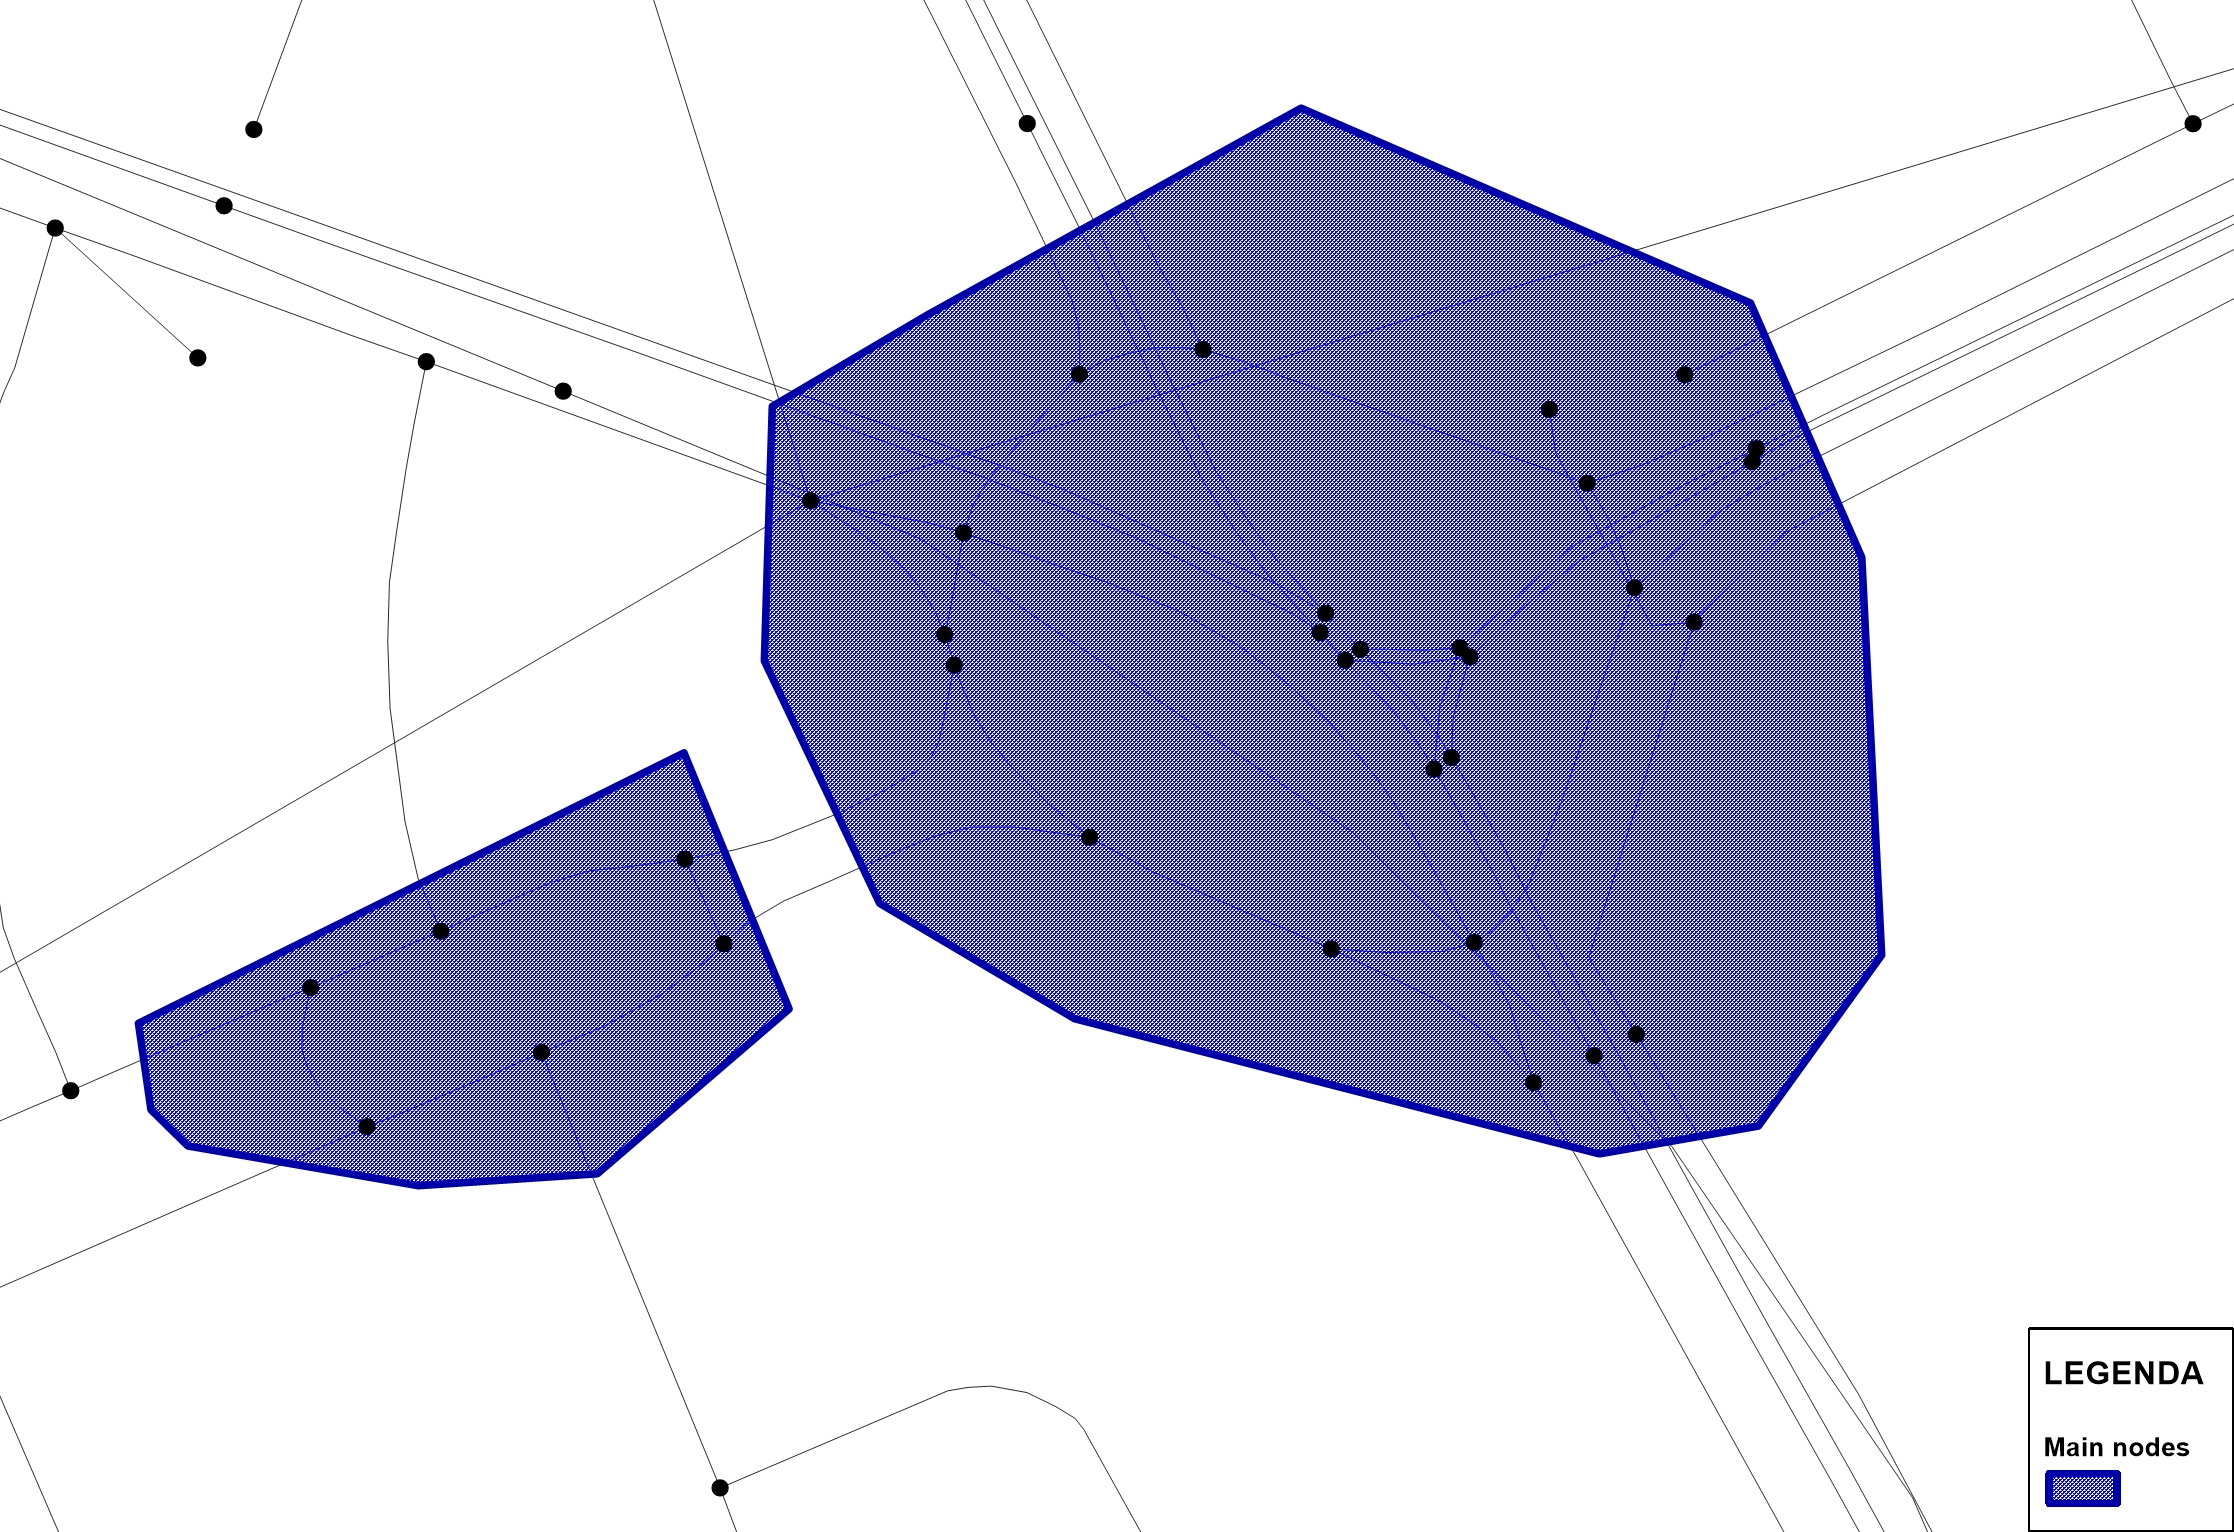
\includegraphics[width=0.9\textwidth]{aggr_node}
 \end{center}  \end{figure} 
\end{frame}


\begin{frame}{Skrzyżowania}{typy}
\begin{figure}\begin{center}
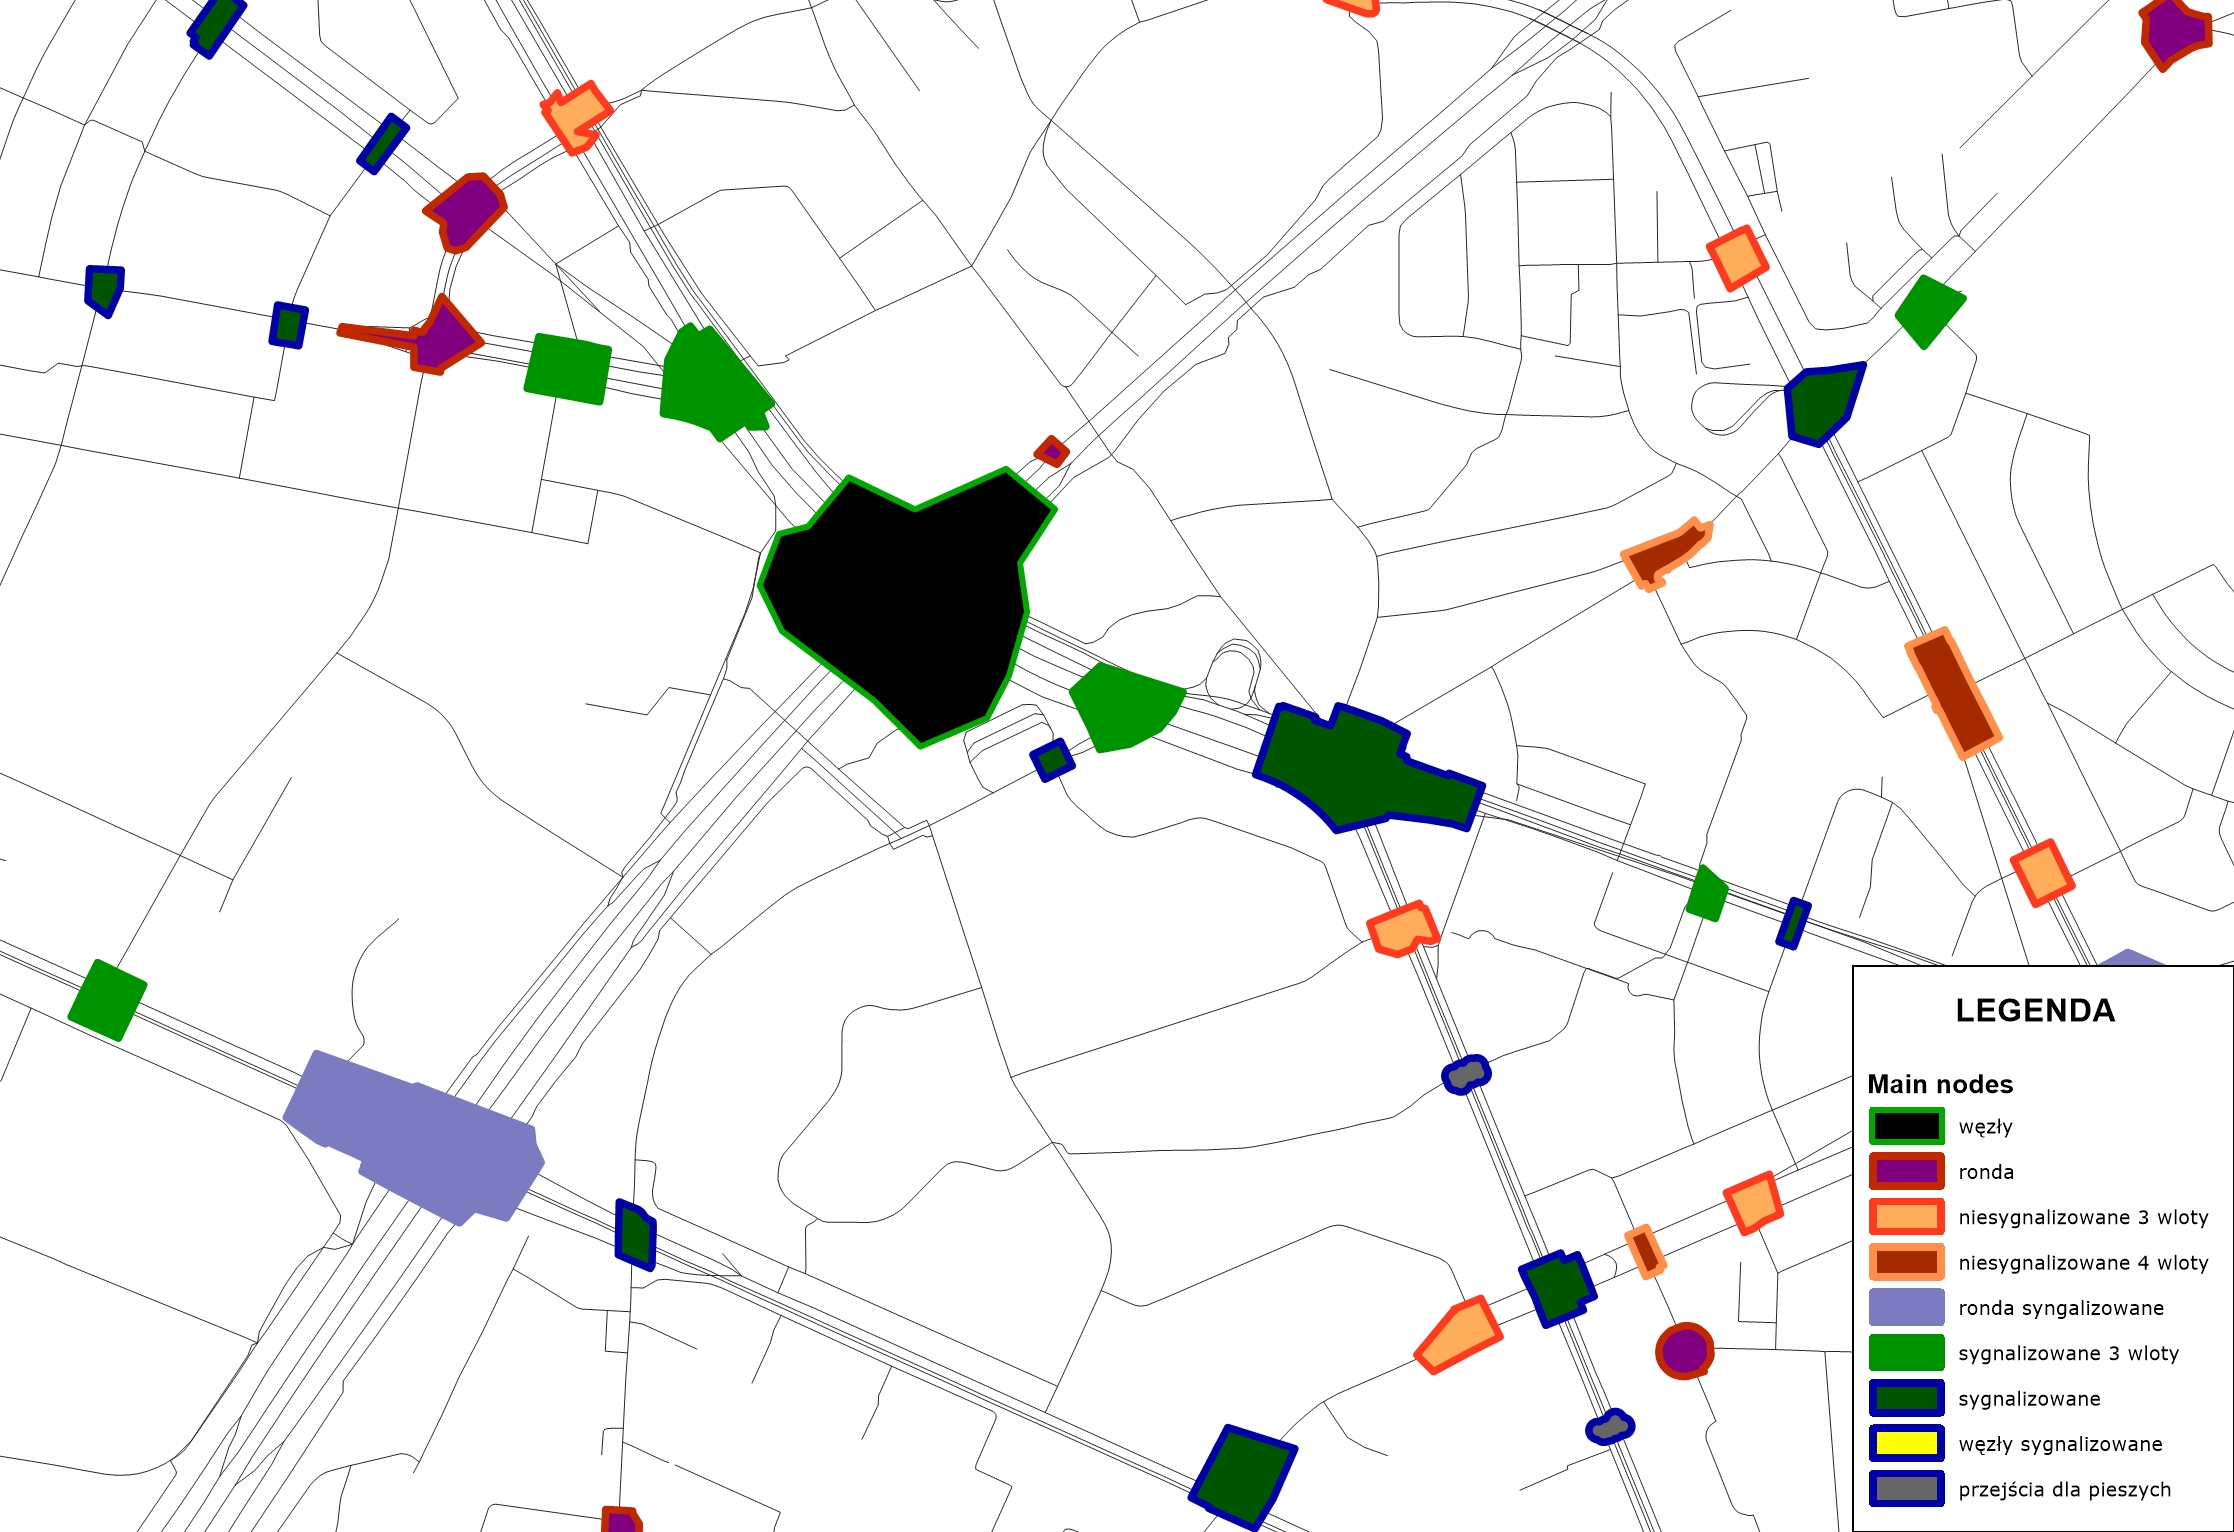
\includegraphics[width=0.9\textwidth]{main_nodes}
 \end{center}  \end{figure} 
\end{frame}

\begin{frame}{Skrzyżowania}{relacje skrętne}
\begin{figure}\begin{center}
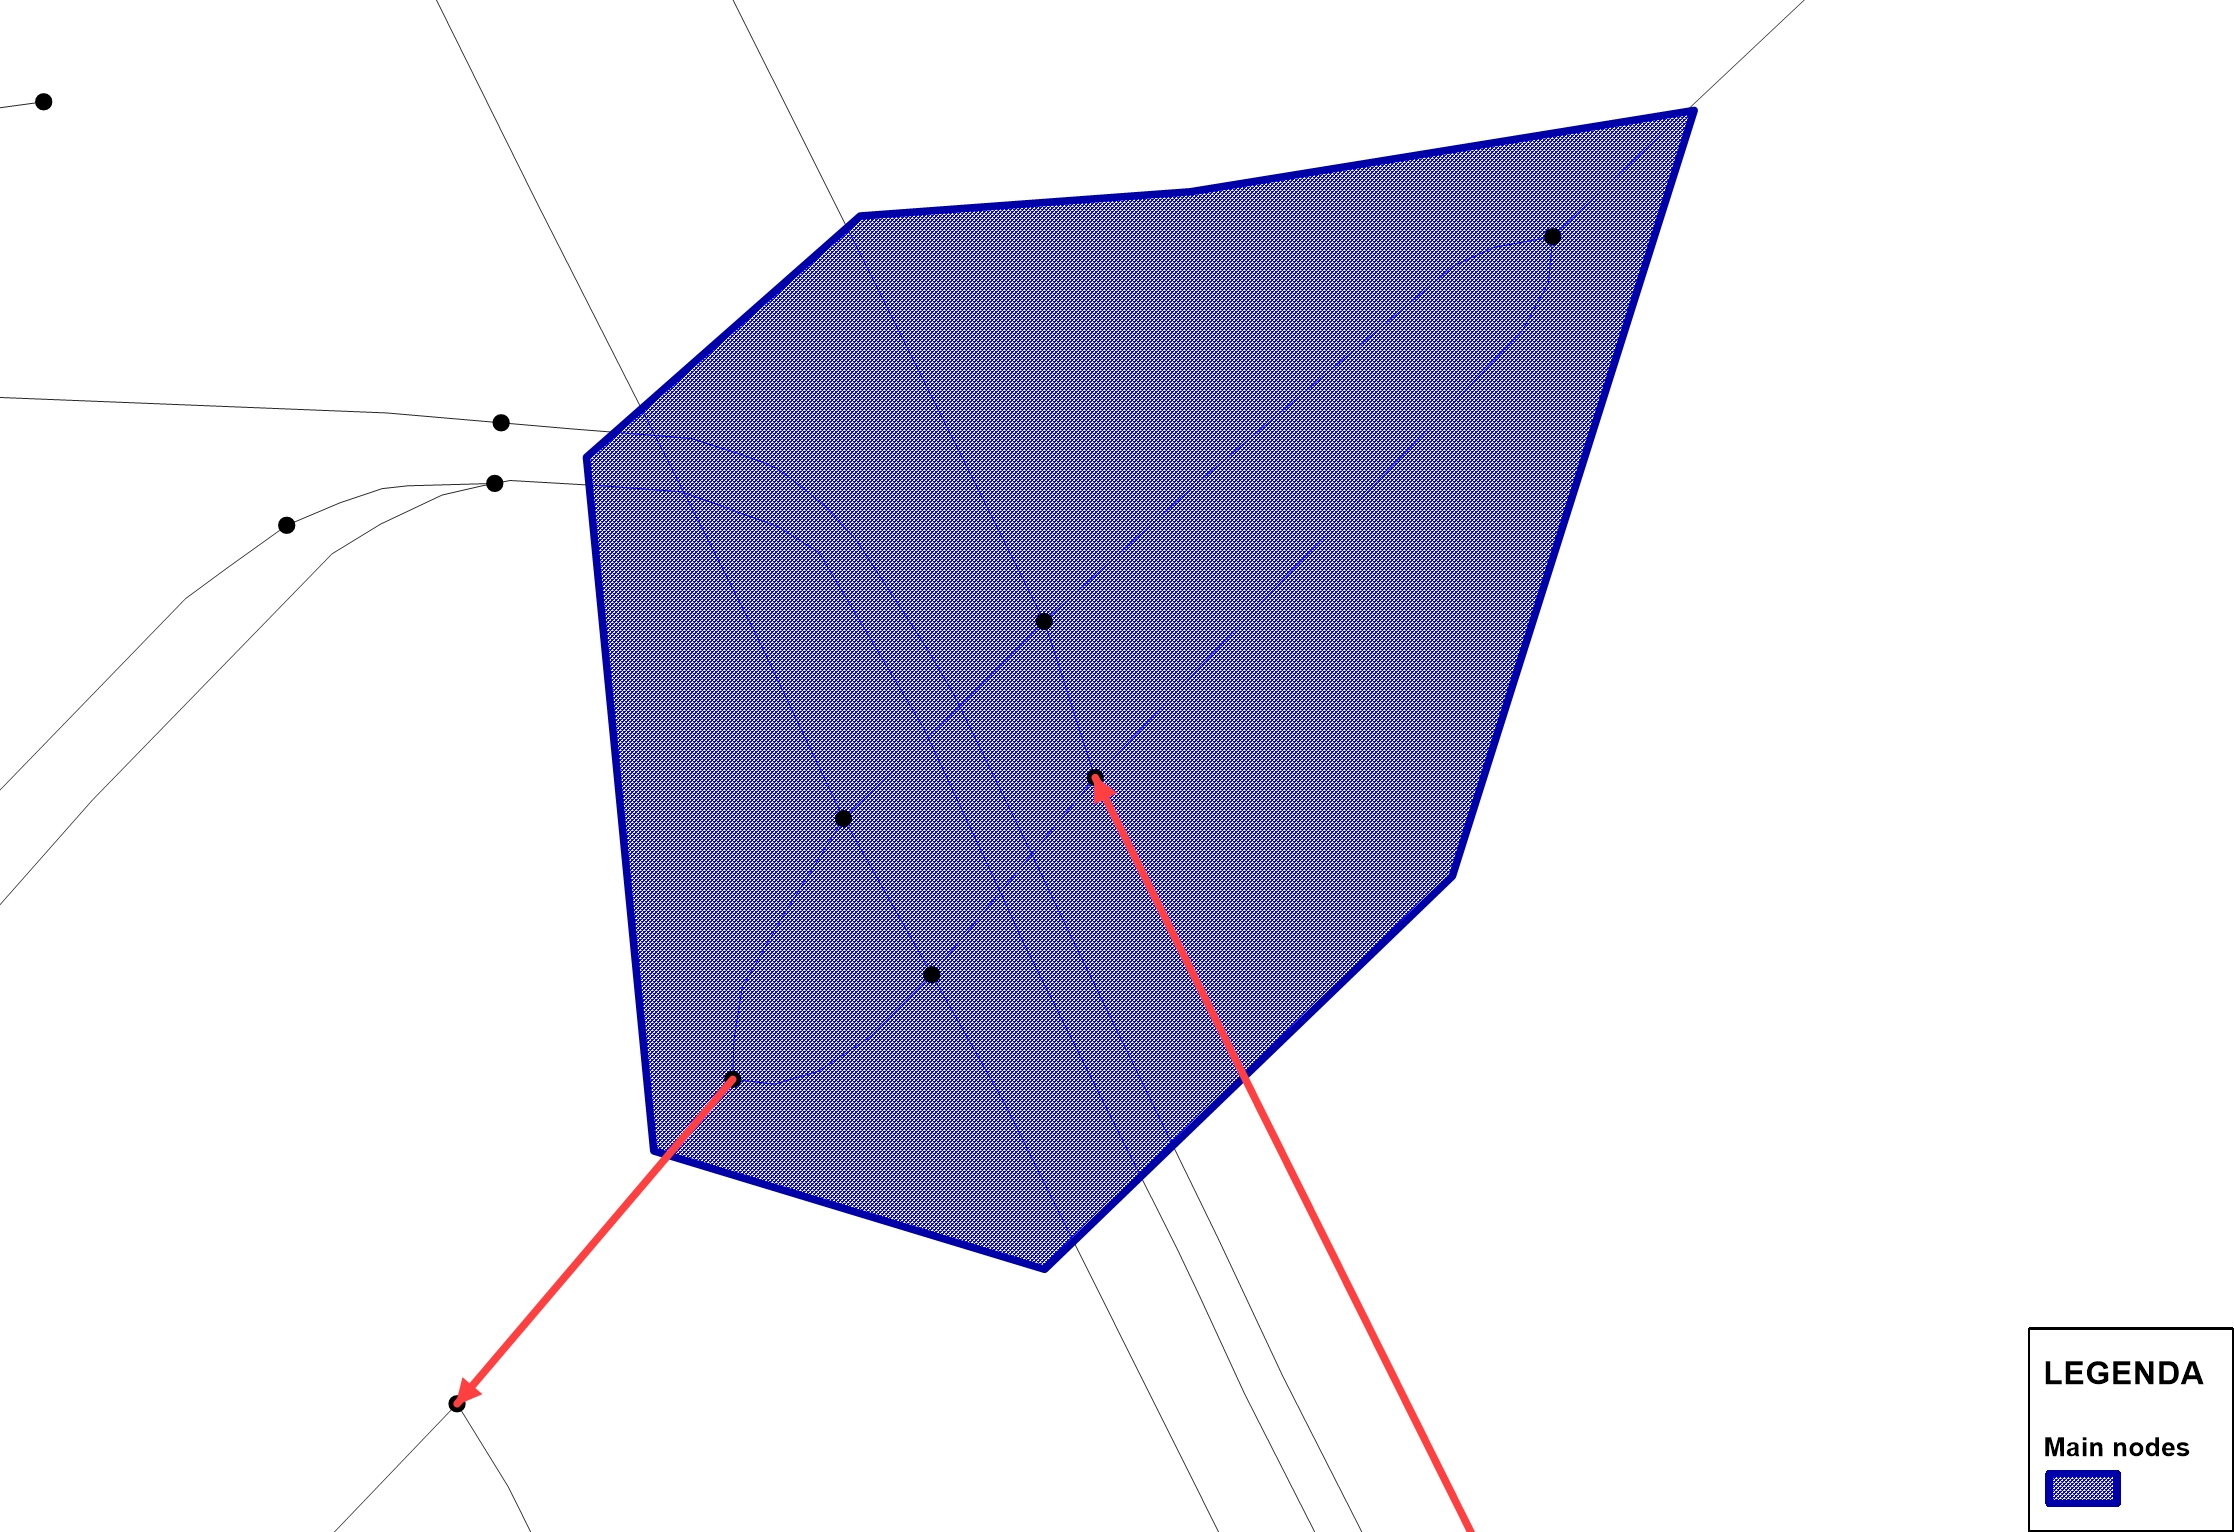
\includegraphics[width=0.9\textwidth]{main_turn}
 \end{center}  \end{figure} 
\end{frame}

\begin{frame}{Skrzyżowania}{edytor graficzny}
\begin{figure}\begin{center}
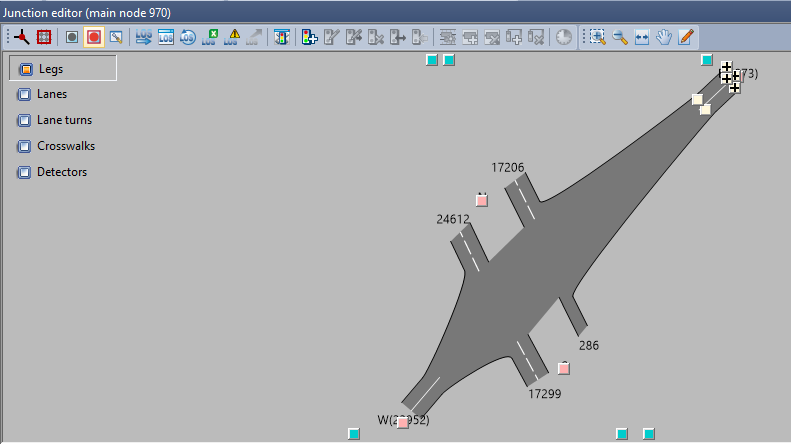
\includegraphics[width=0.9\textwidth]{geom_editor}
 \end{center}  \end{figure} 
\end{frame}

\begin{frame}{Skrzyżowania}{edytor relacji}
\begin{figure}\begin{center}
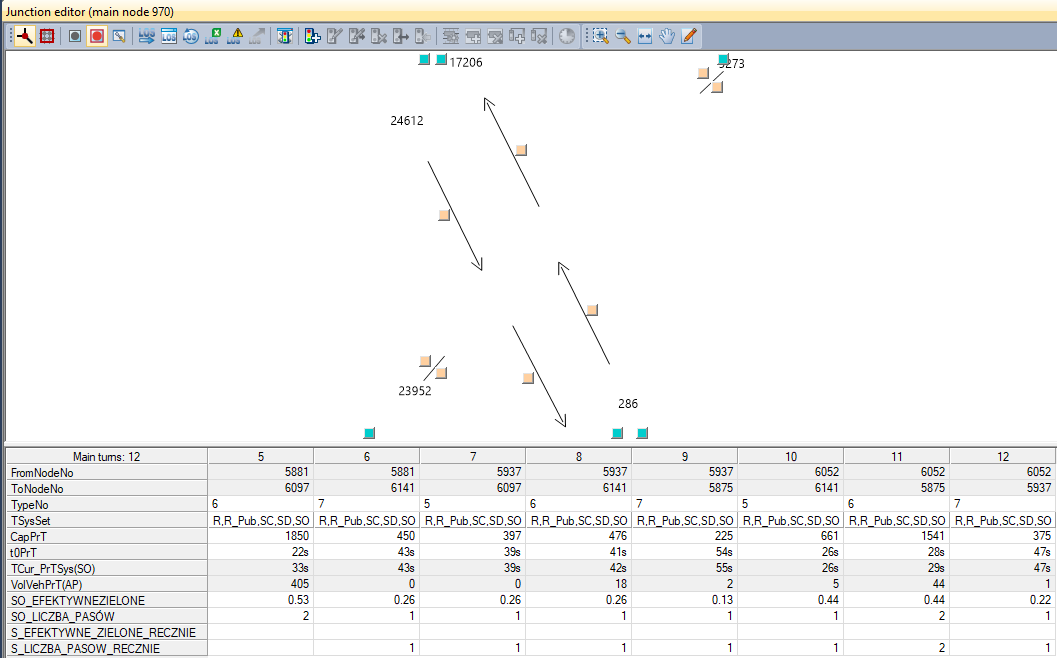
\includegraphics[width=0.9\textwidth]{junction_editor}
 \end{center}  \end{figure} 
\end{frame}

\begin{frame}{Metoda Obliczania Przepustowości}{algorytm}
\begin{figure}\begin{center}
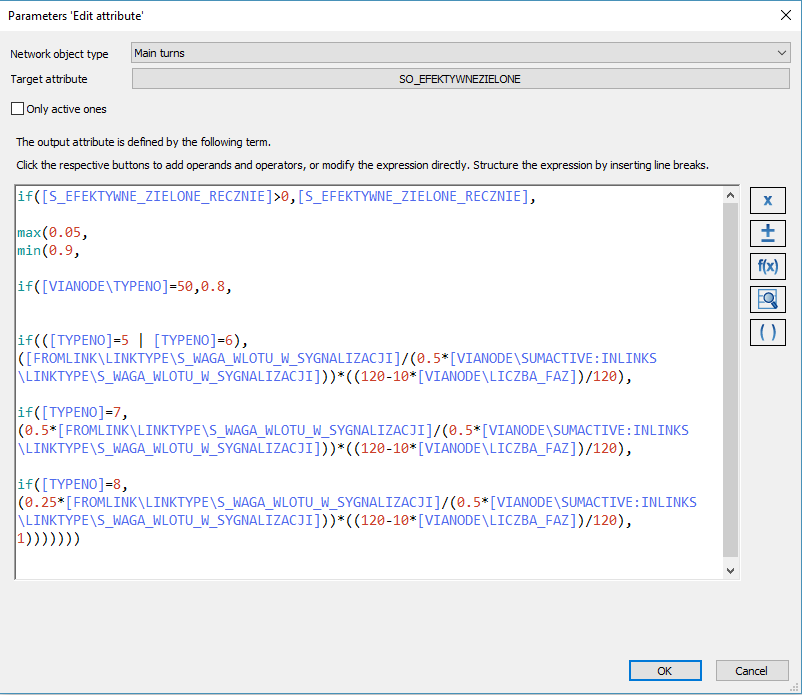
\includegraphics[width=0.9\textwidth]{algo}
 \end{center}  \end{figure} 
\end{frame}

\begin{frame}{Metoda Obliczania Przepustowości}{algorytm}
\begin{figure}\begin{center}
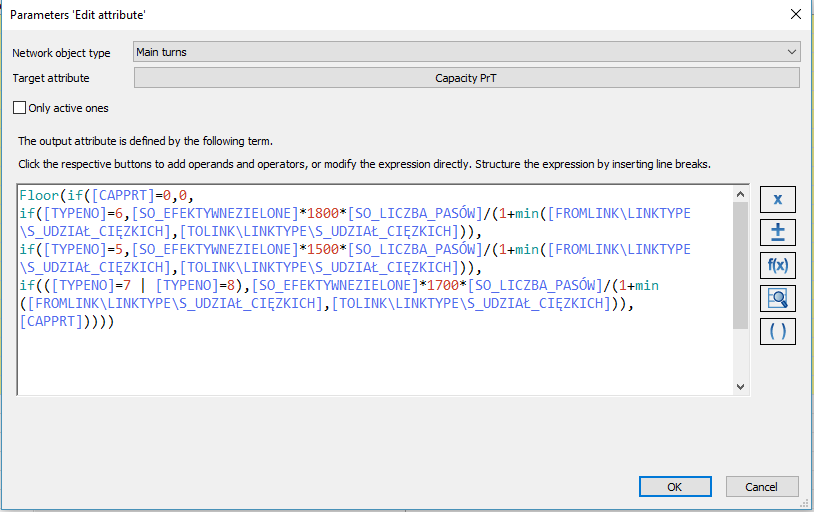
\includegraphics[width=0.9\textwidth]{algo2}
 \end{center}  \end{figure} 
\end{frame}

\section{Szukanie najkrótszej ścieżki}
\begin{frame}{Opór w sieci}{impedancja}
\begin{figure}\begin{center}
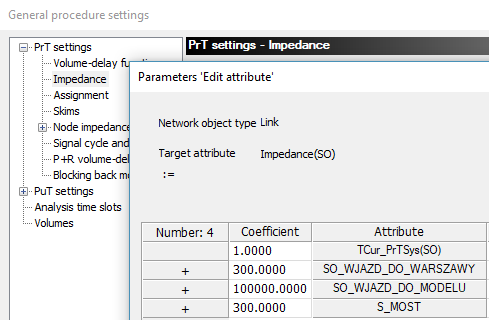
\includegraphics[width=0.5\textwidth]{imp}
 \end{center}  \end{figure} 
\end{frame}

\begin{frame}{Najkrótsza ścieżka}{odległość}
\begin{figure}\begin{center}
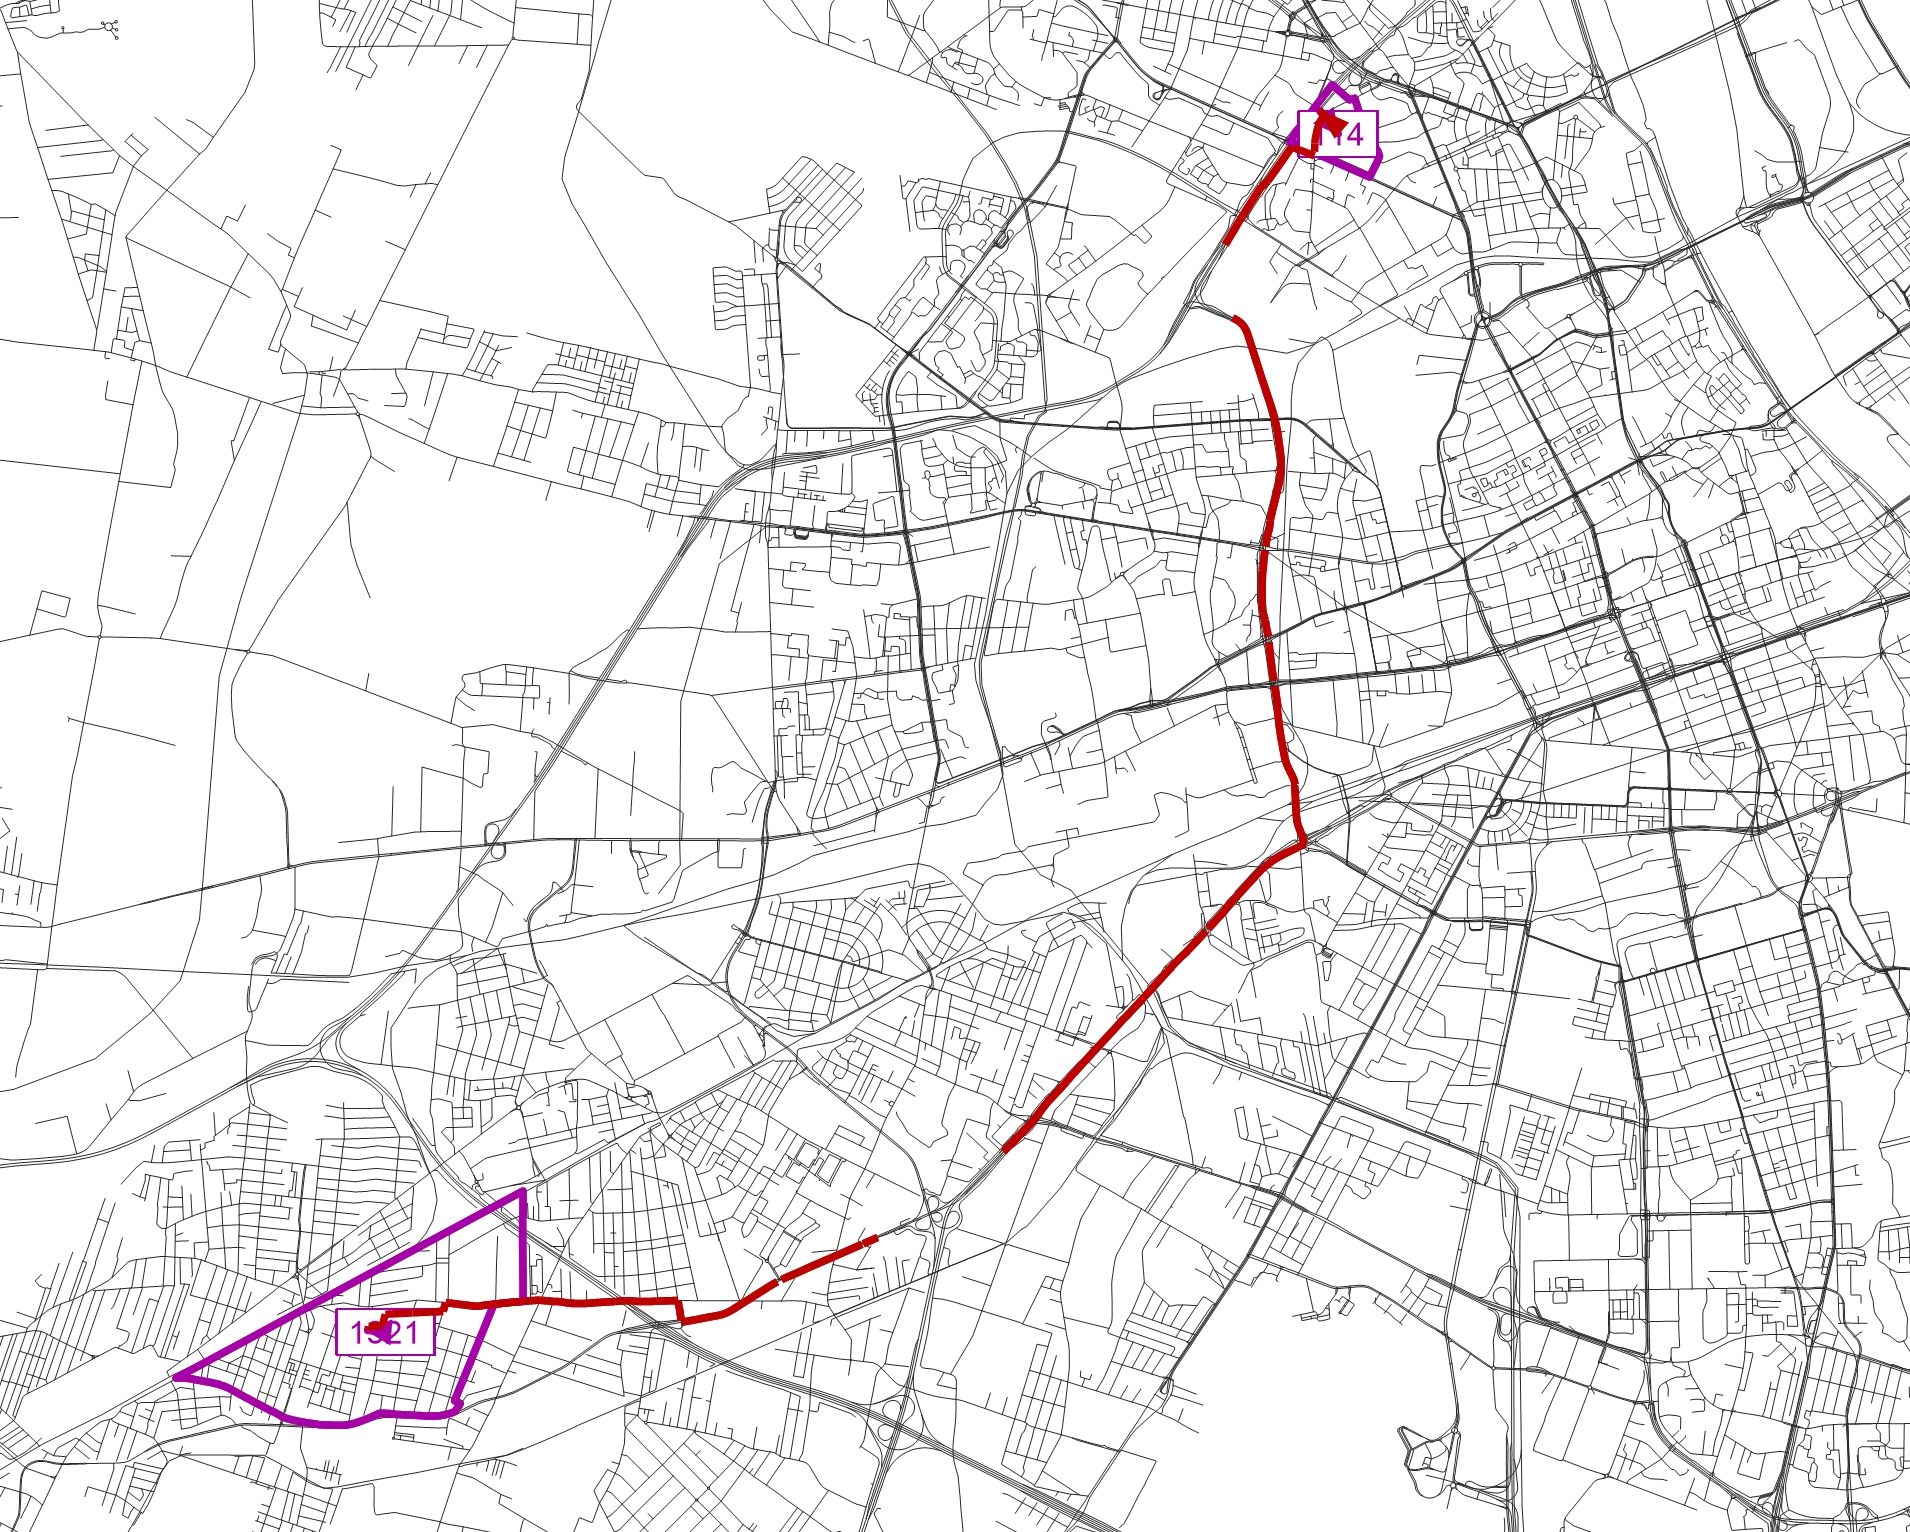
\includegraphics[width=0.8\textwidth]{path_dist}
 \end{center}  \end{figure} 
\end{frame}

\begin{frame}{Najkrótsza ścieżka}{czas}
\begin{figure}\begin{center}
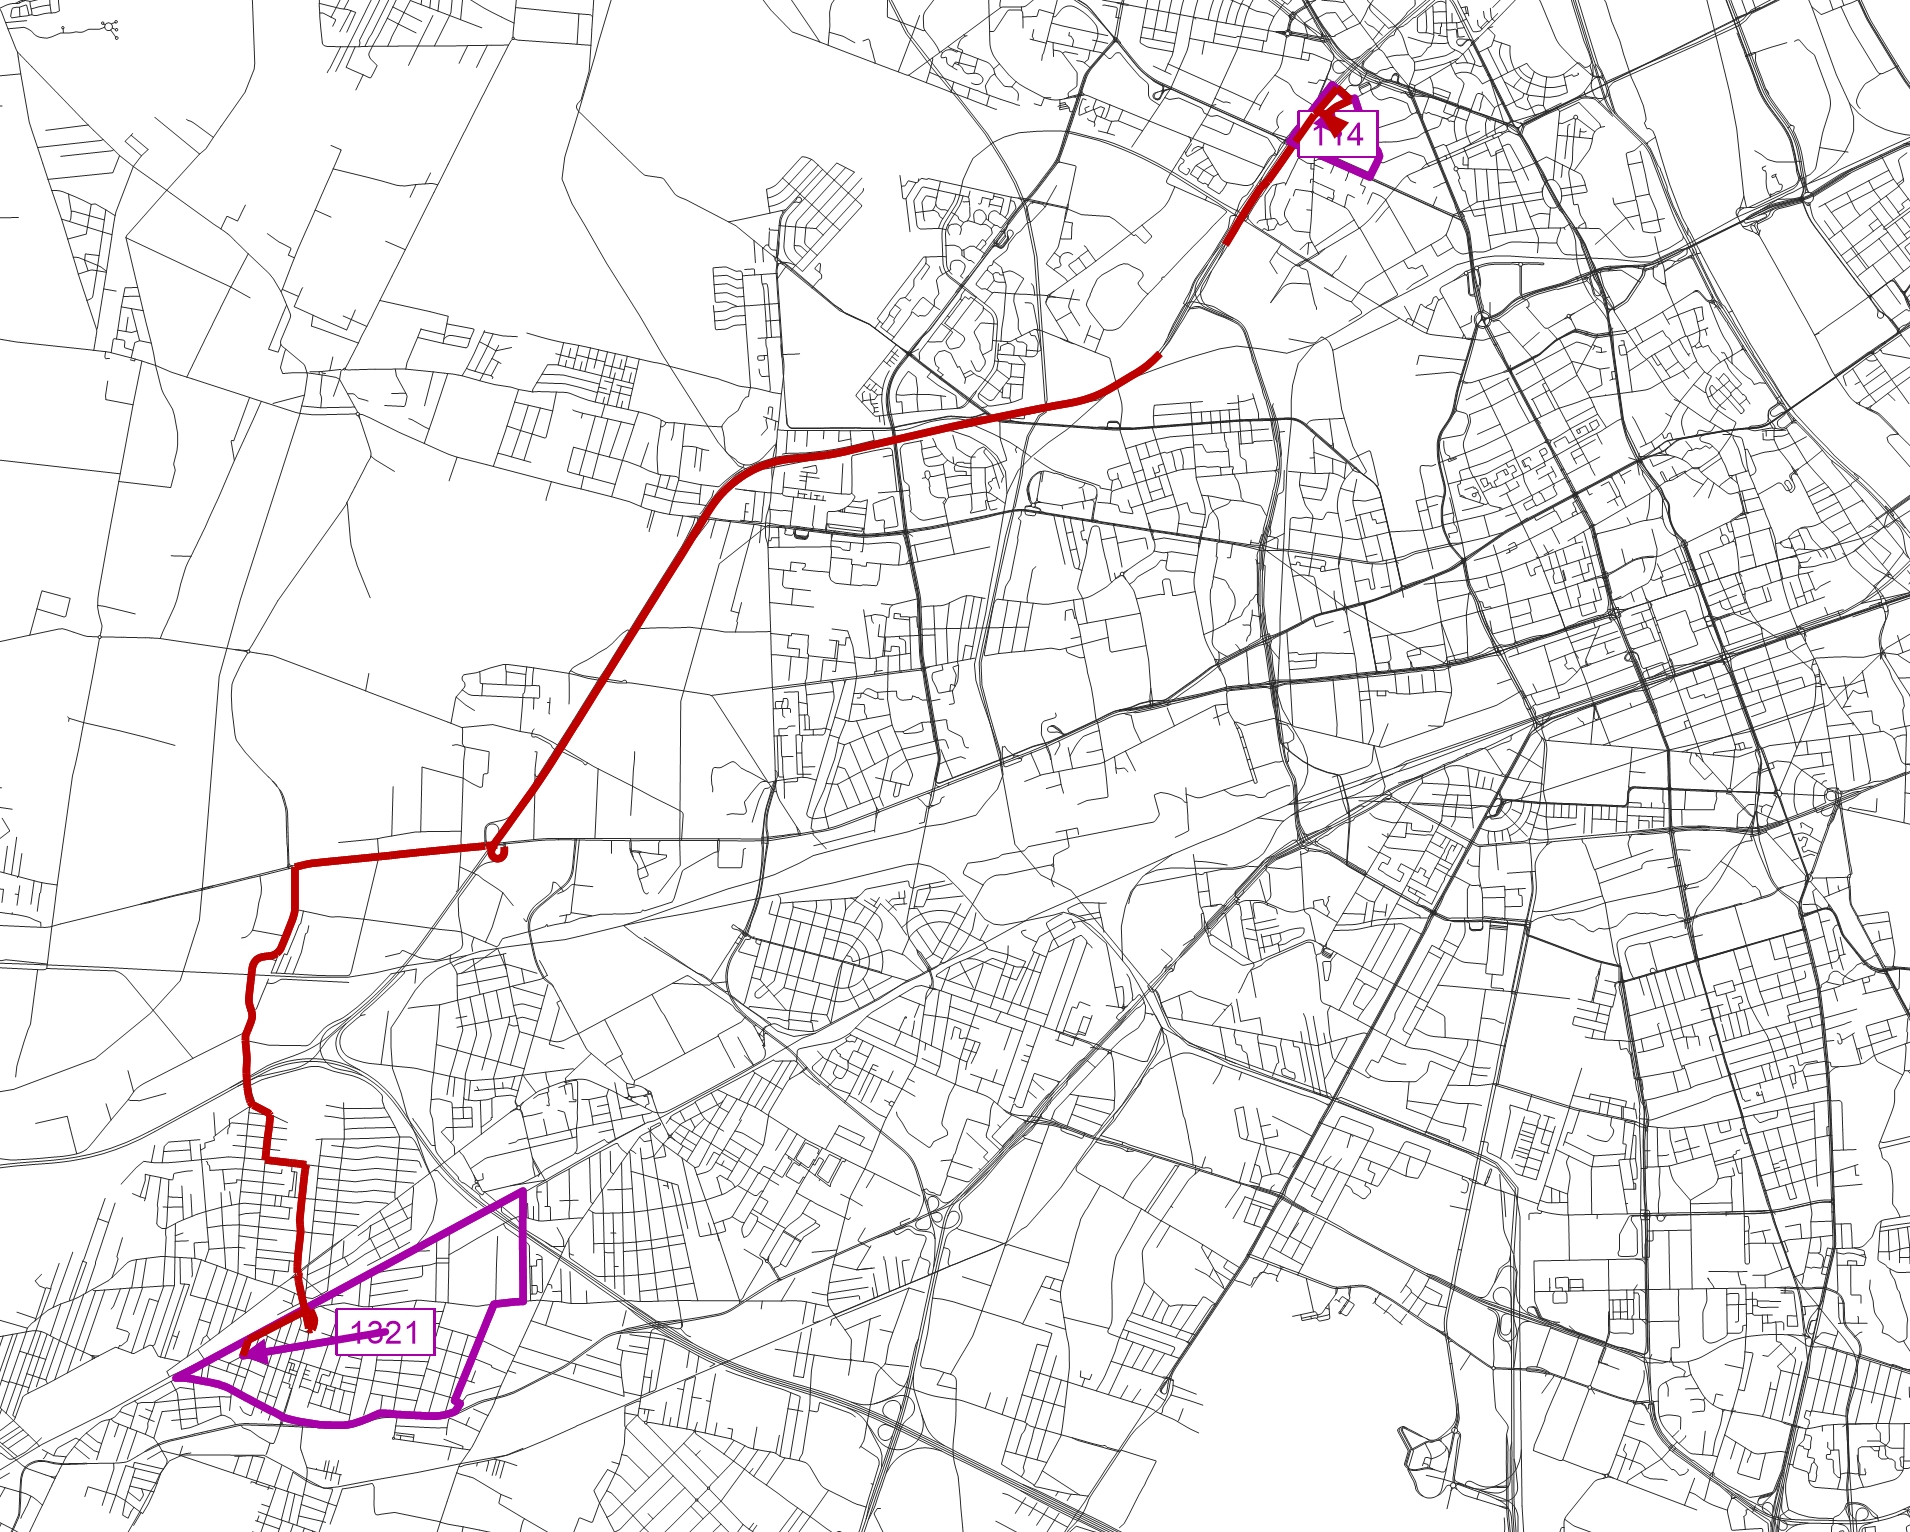
\includegraphics[width=0.8\textwidth]{path_time}
 \end{center}  \end{figure} 
\end{frame}

\begin{frame}{Najkrótsza ścieżka}{czas w zatłoczonej sieci}
\begin{figure}\begin{center}
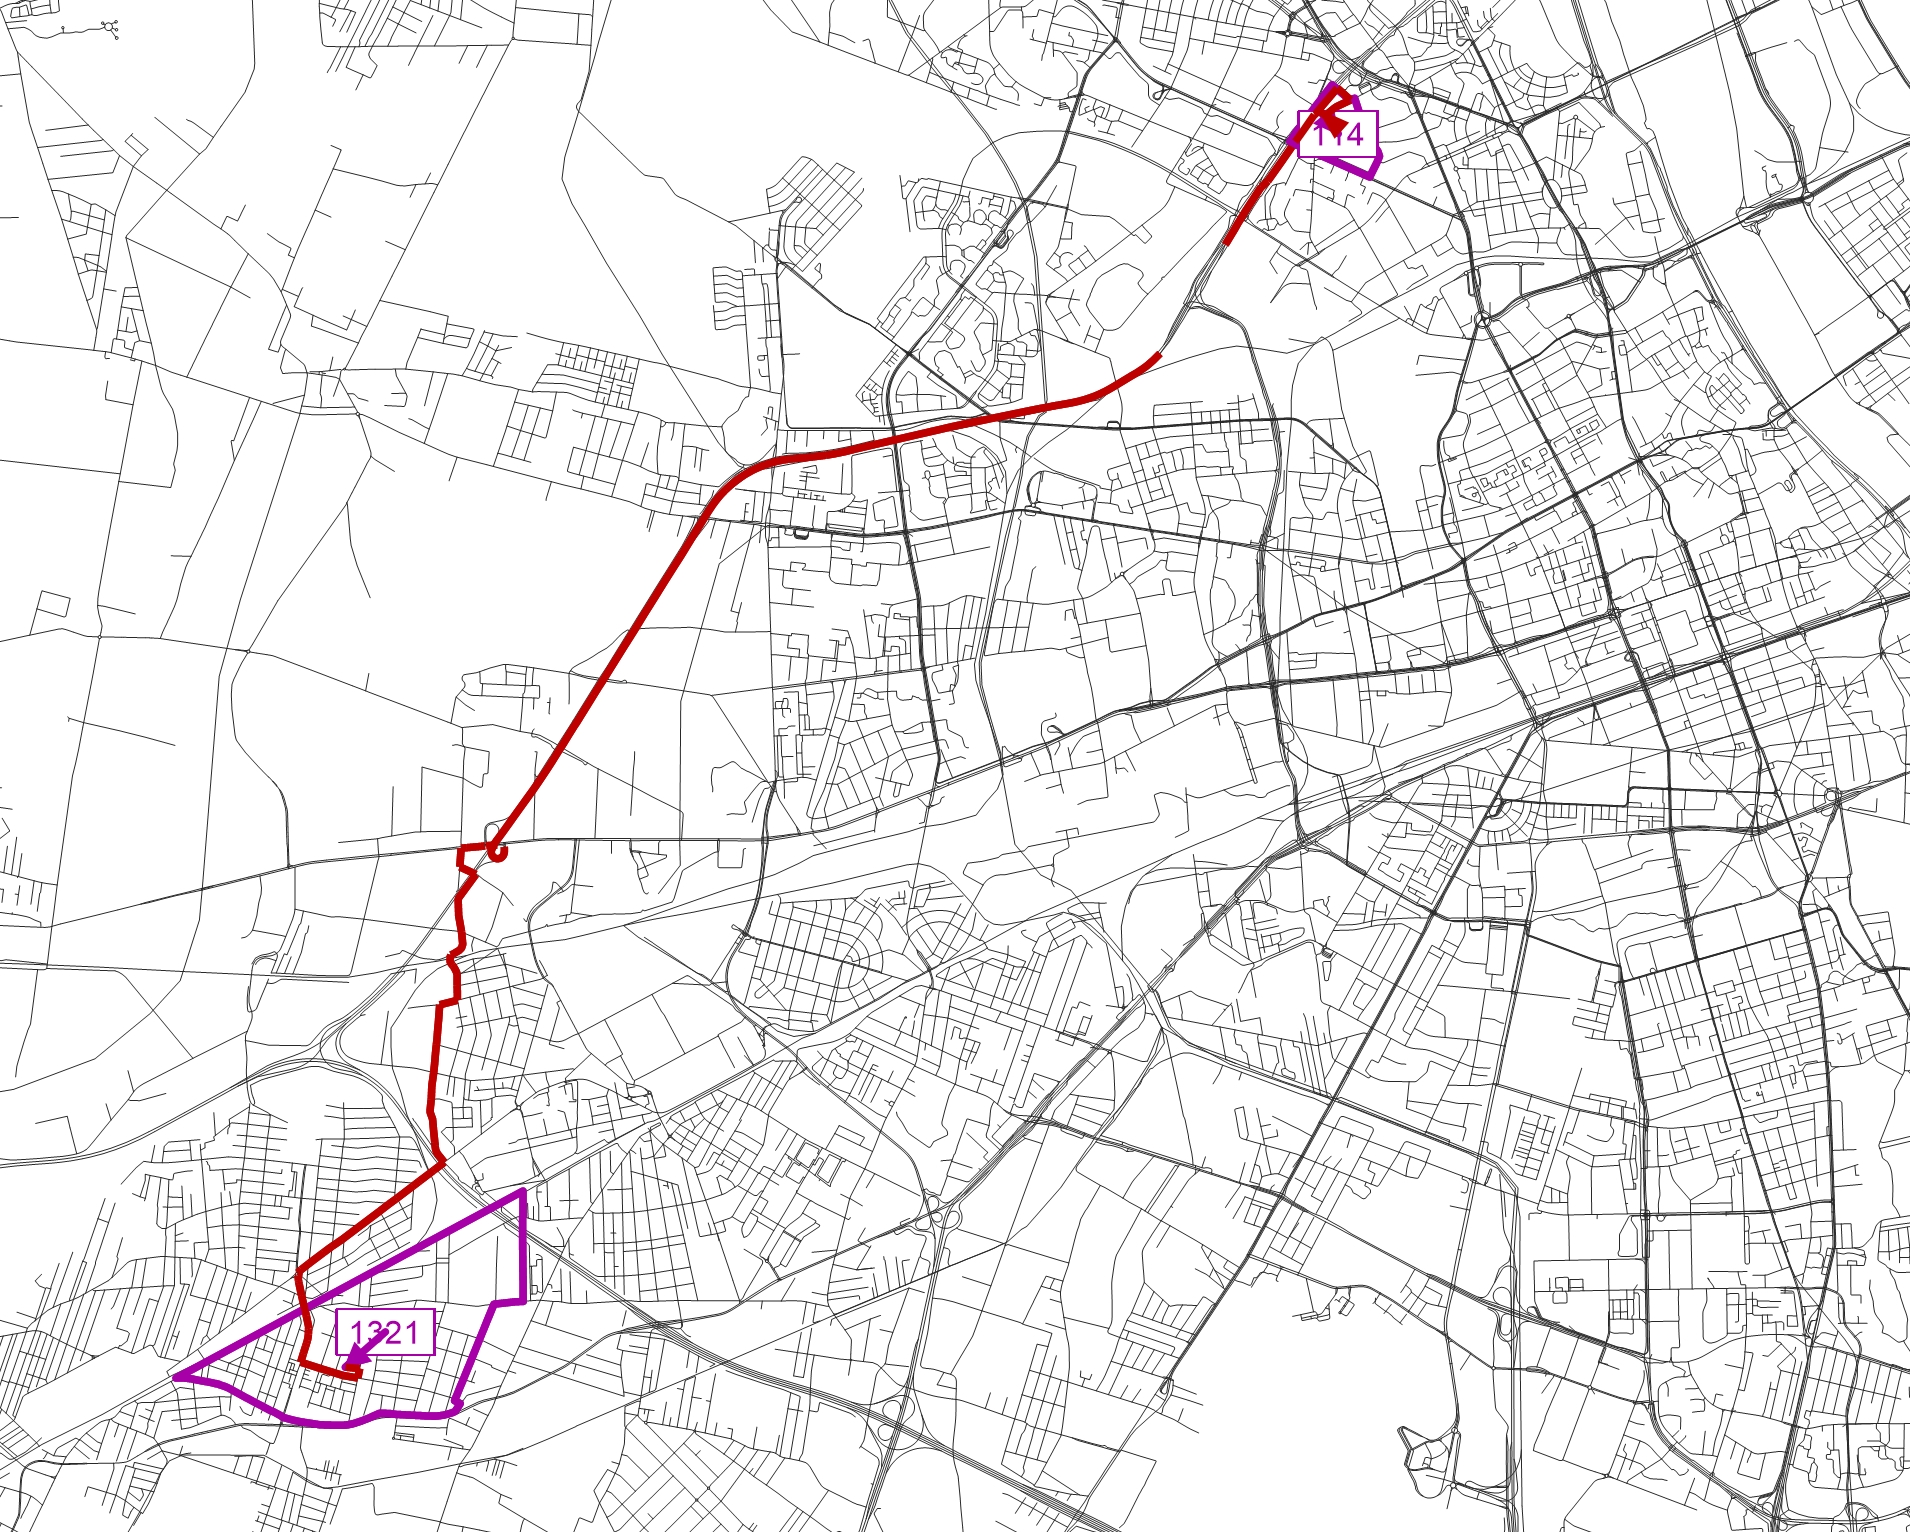
\includegraphics[width=0.8\textwidth]{path_jam}
 \end{center}  \end{figure} 
\end{frame}

\begin{frame}{Najkrótsza ścieżka}{komunikacja zbiorowa rano}
\begin{figure}\begin{center}
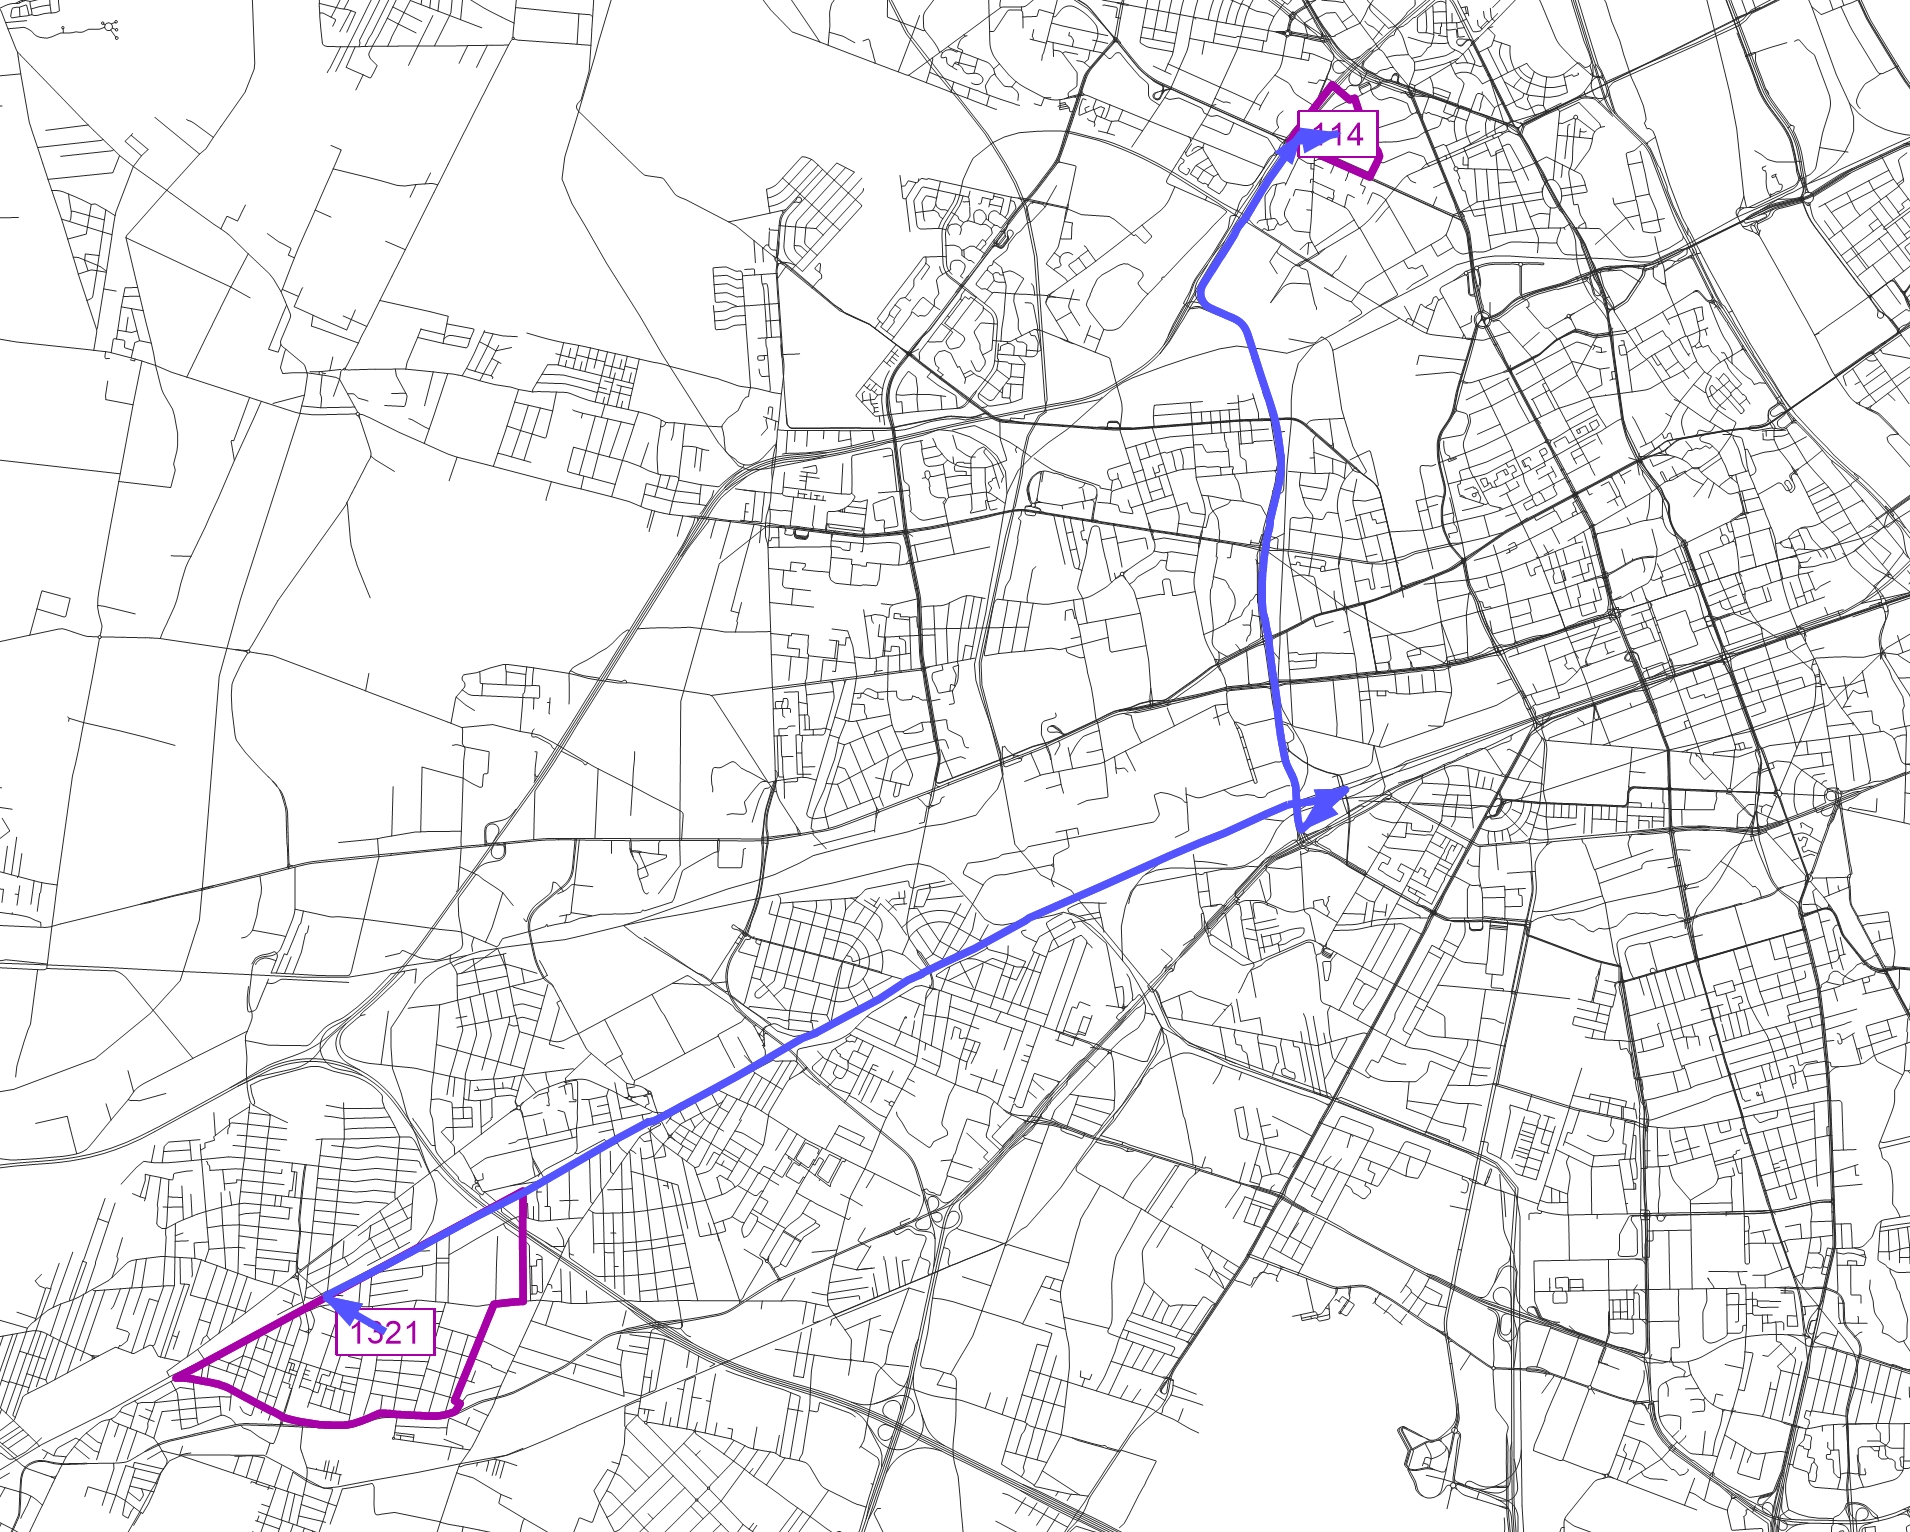
\includegraphics[width=0.8\textwidth]{path_transit}
 \end{center}  \end{figure} 
\end{frame}

\begin{frame}{Najkrótsza ścieżka}{komunikacja zbiorowa wieczór}
\begin{figure}\begin{center}
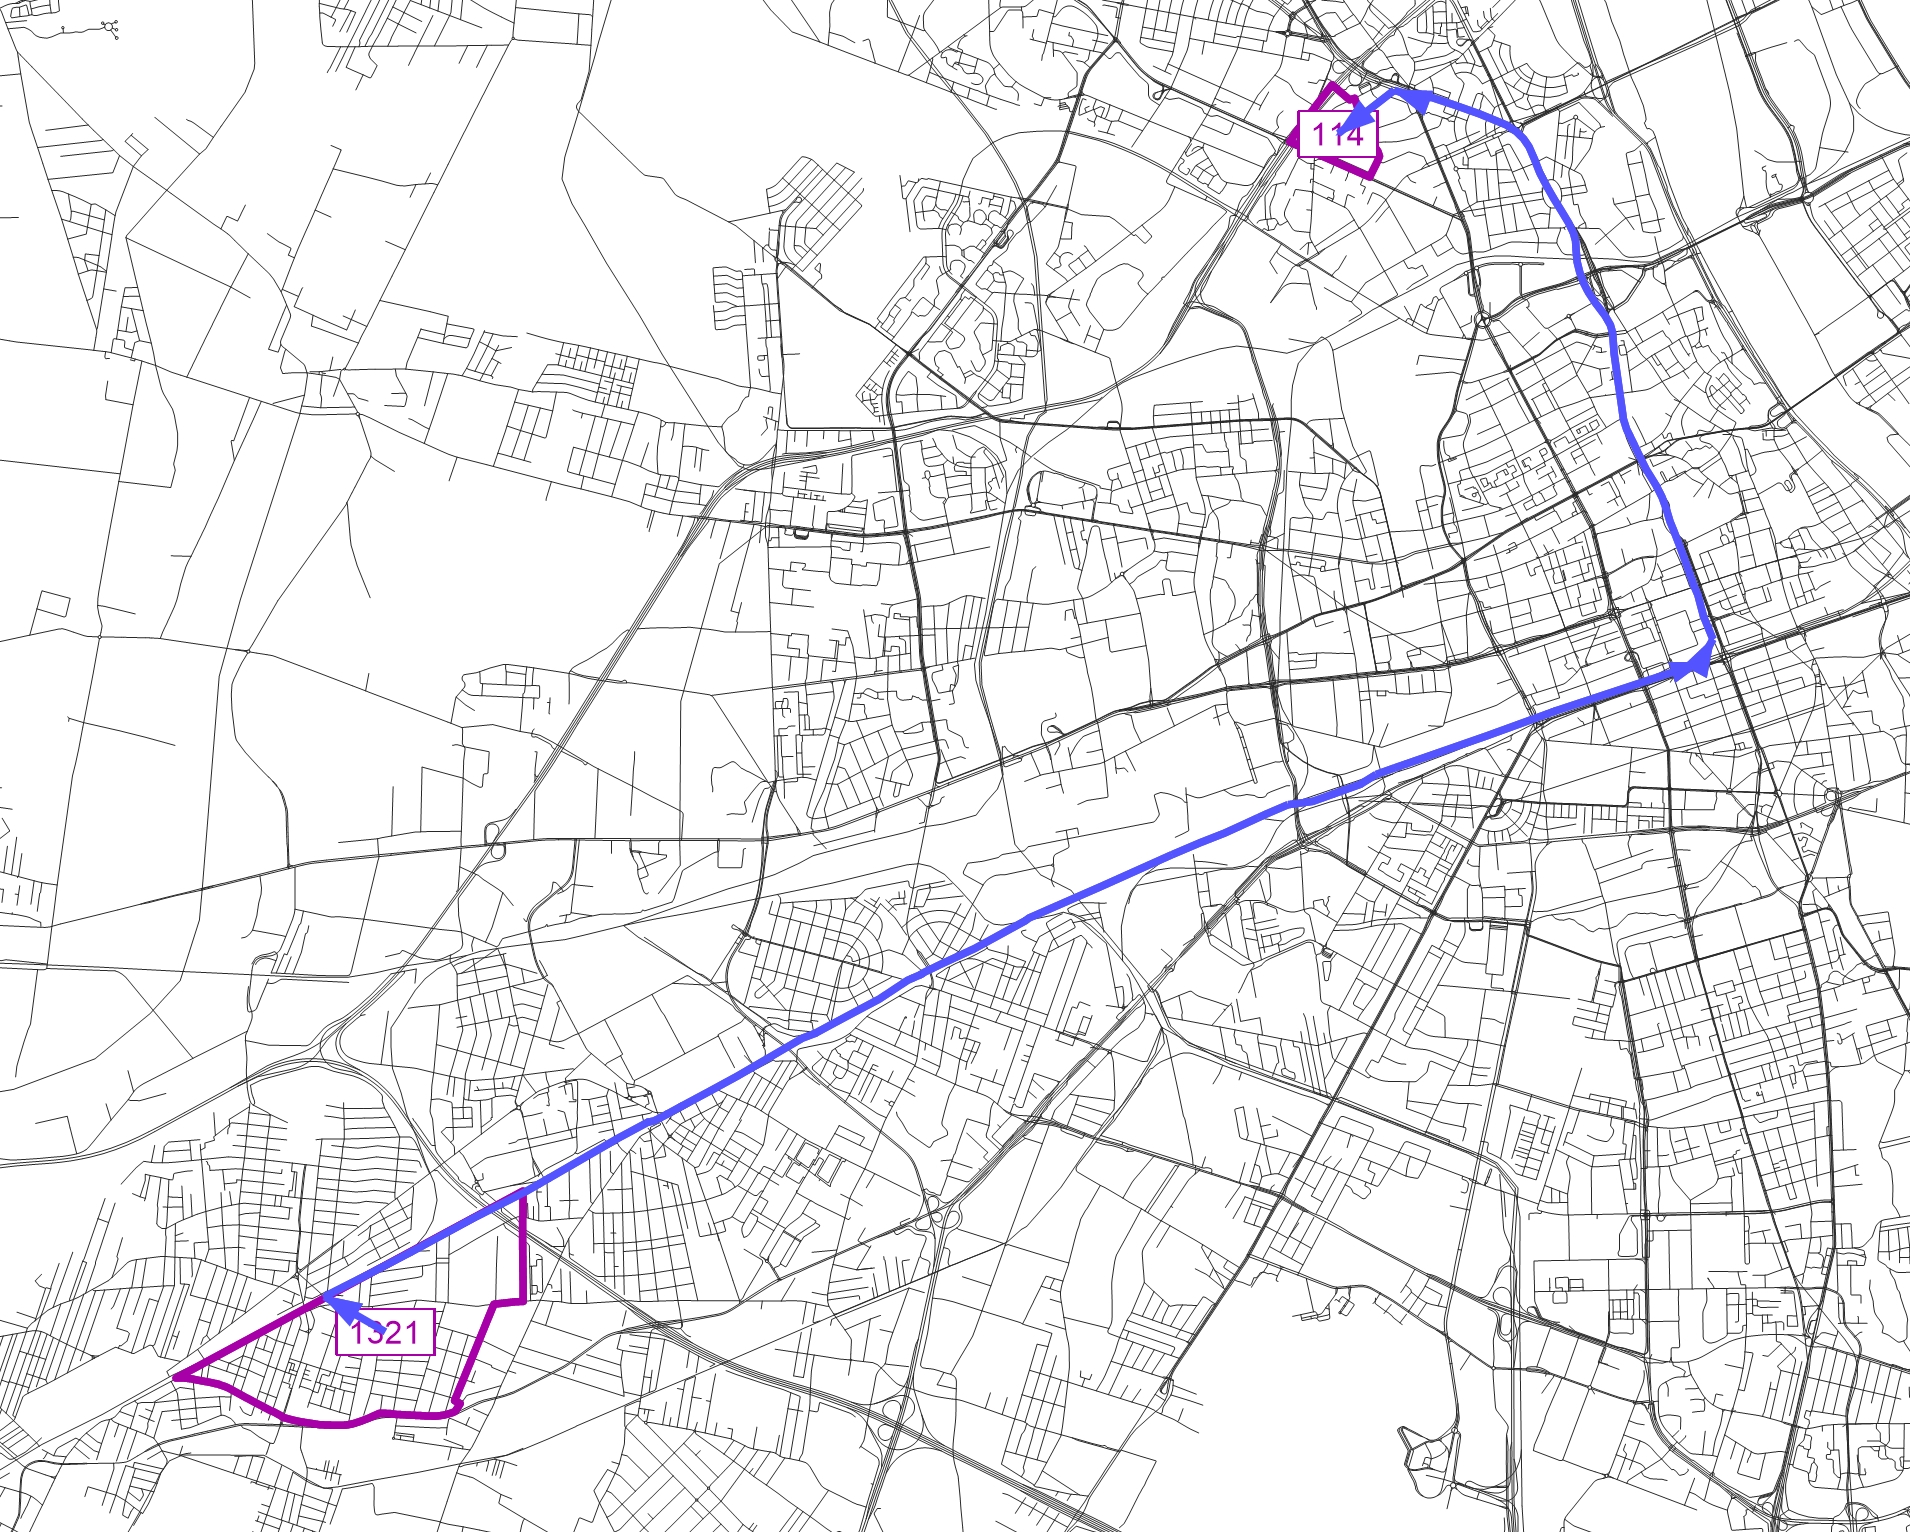
\includegraphics[width=0.8\textwidth]{path_transit2}
 \end{center}  \end{figure} 
\end{frame}

\section{Model popytu}
\subsection{Rejony komunikacyjne}
\begin{frame}{Rejony}
\begin{figure}\begin{center}
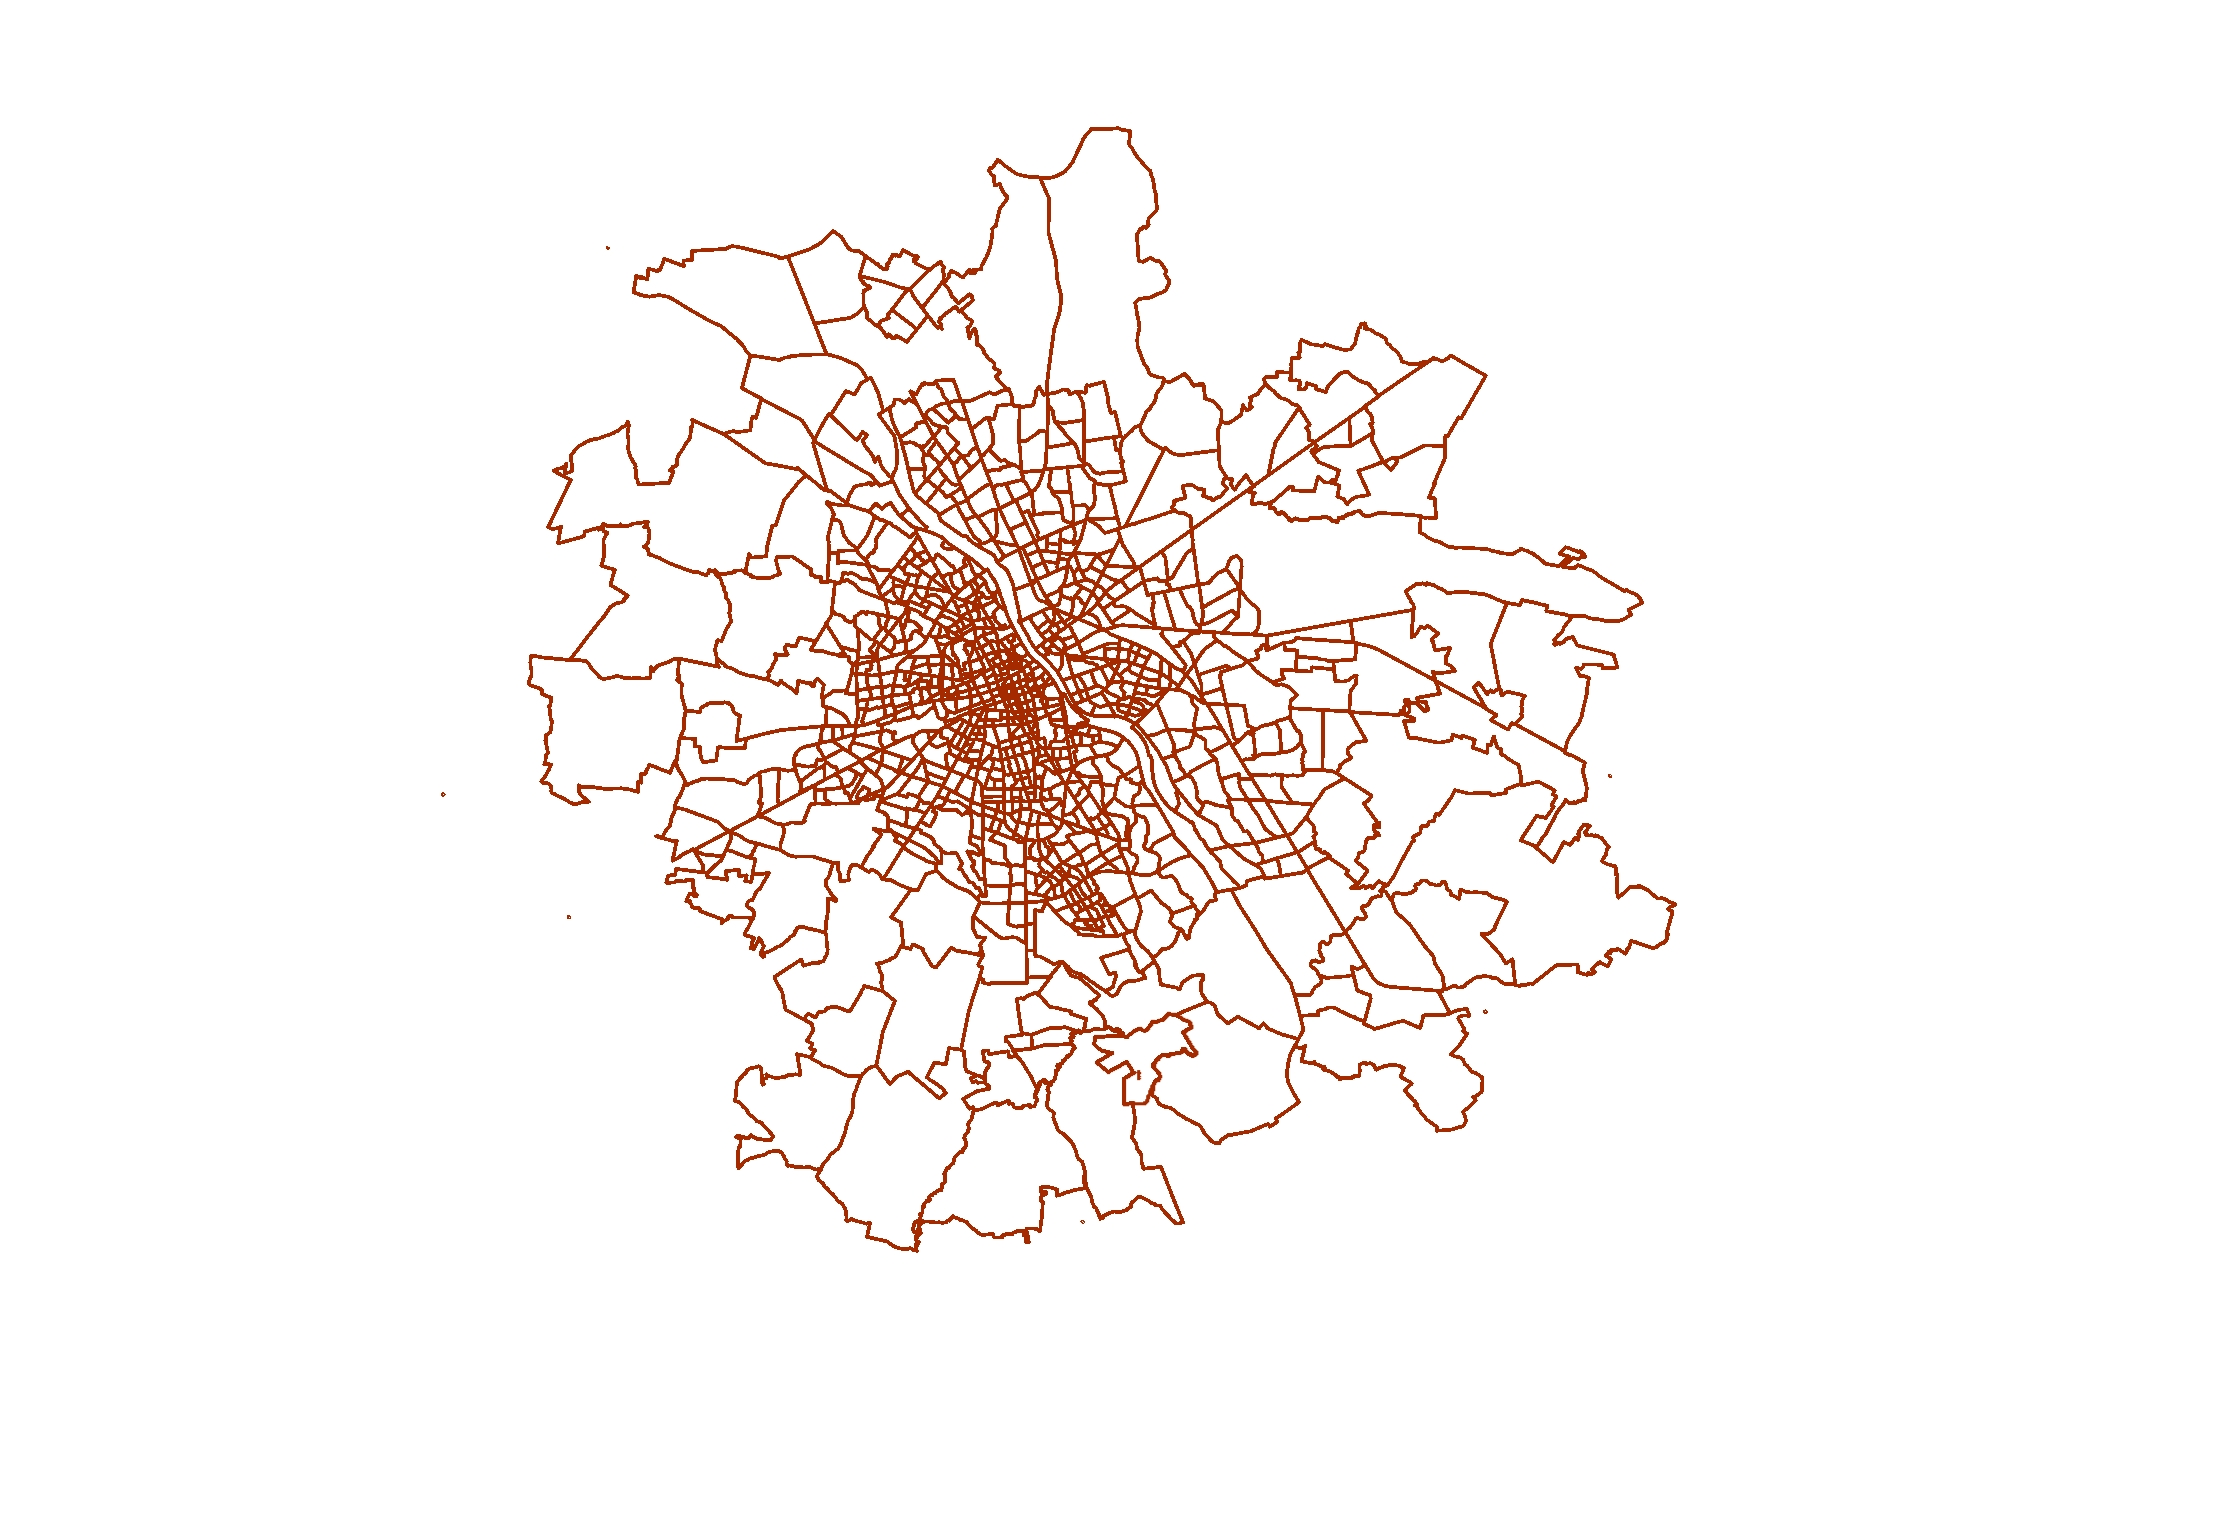
\includegraphics[width=0.9\textwidth]{zones1}
 \end{center}  \end{figure} 
\end{frame}

\begin{frame}{Rejony}
\begin{figure}\begin{center}
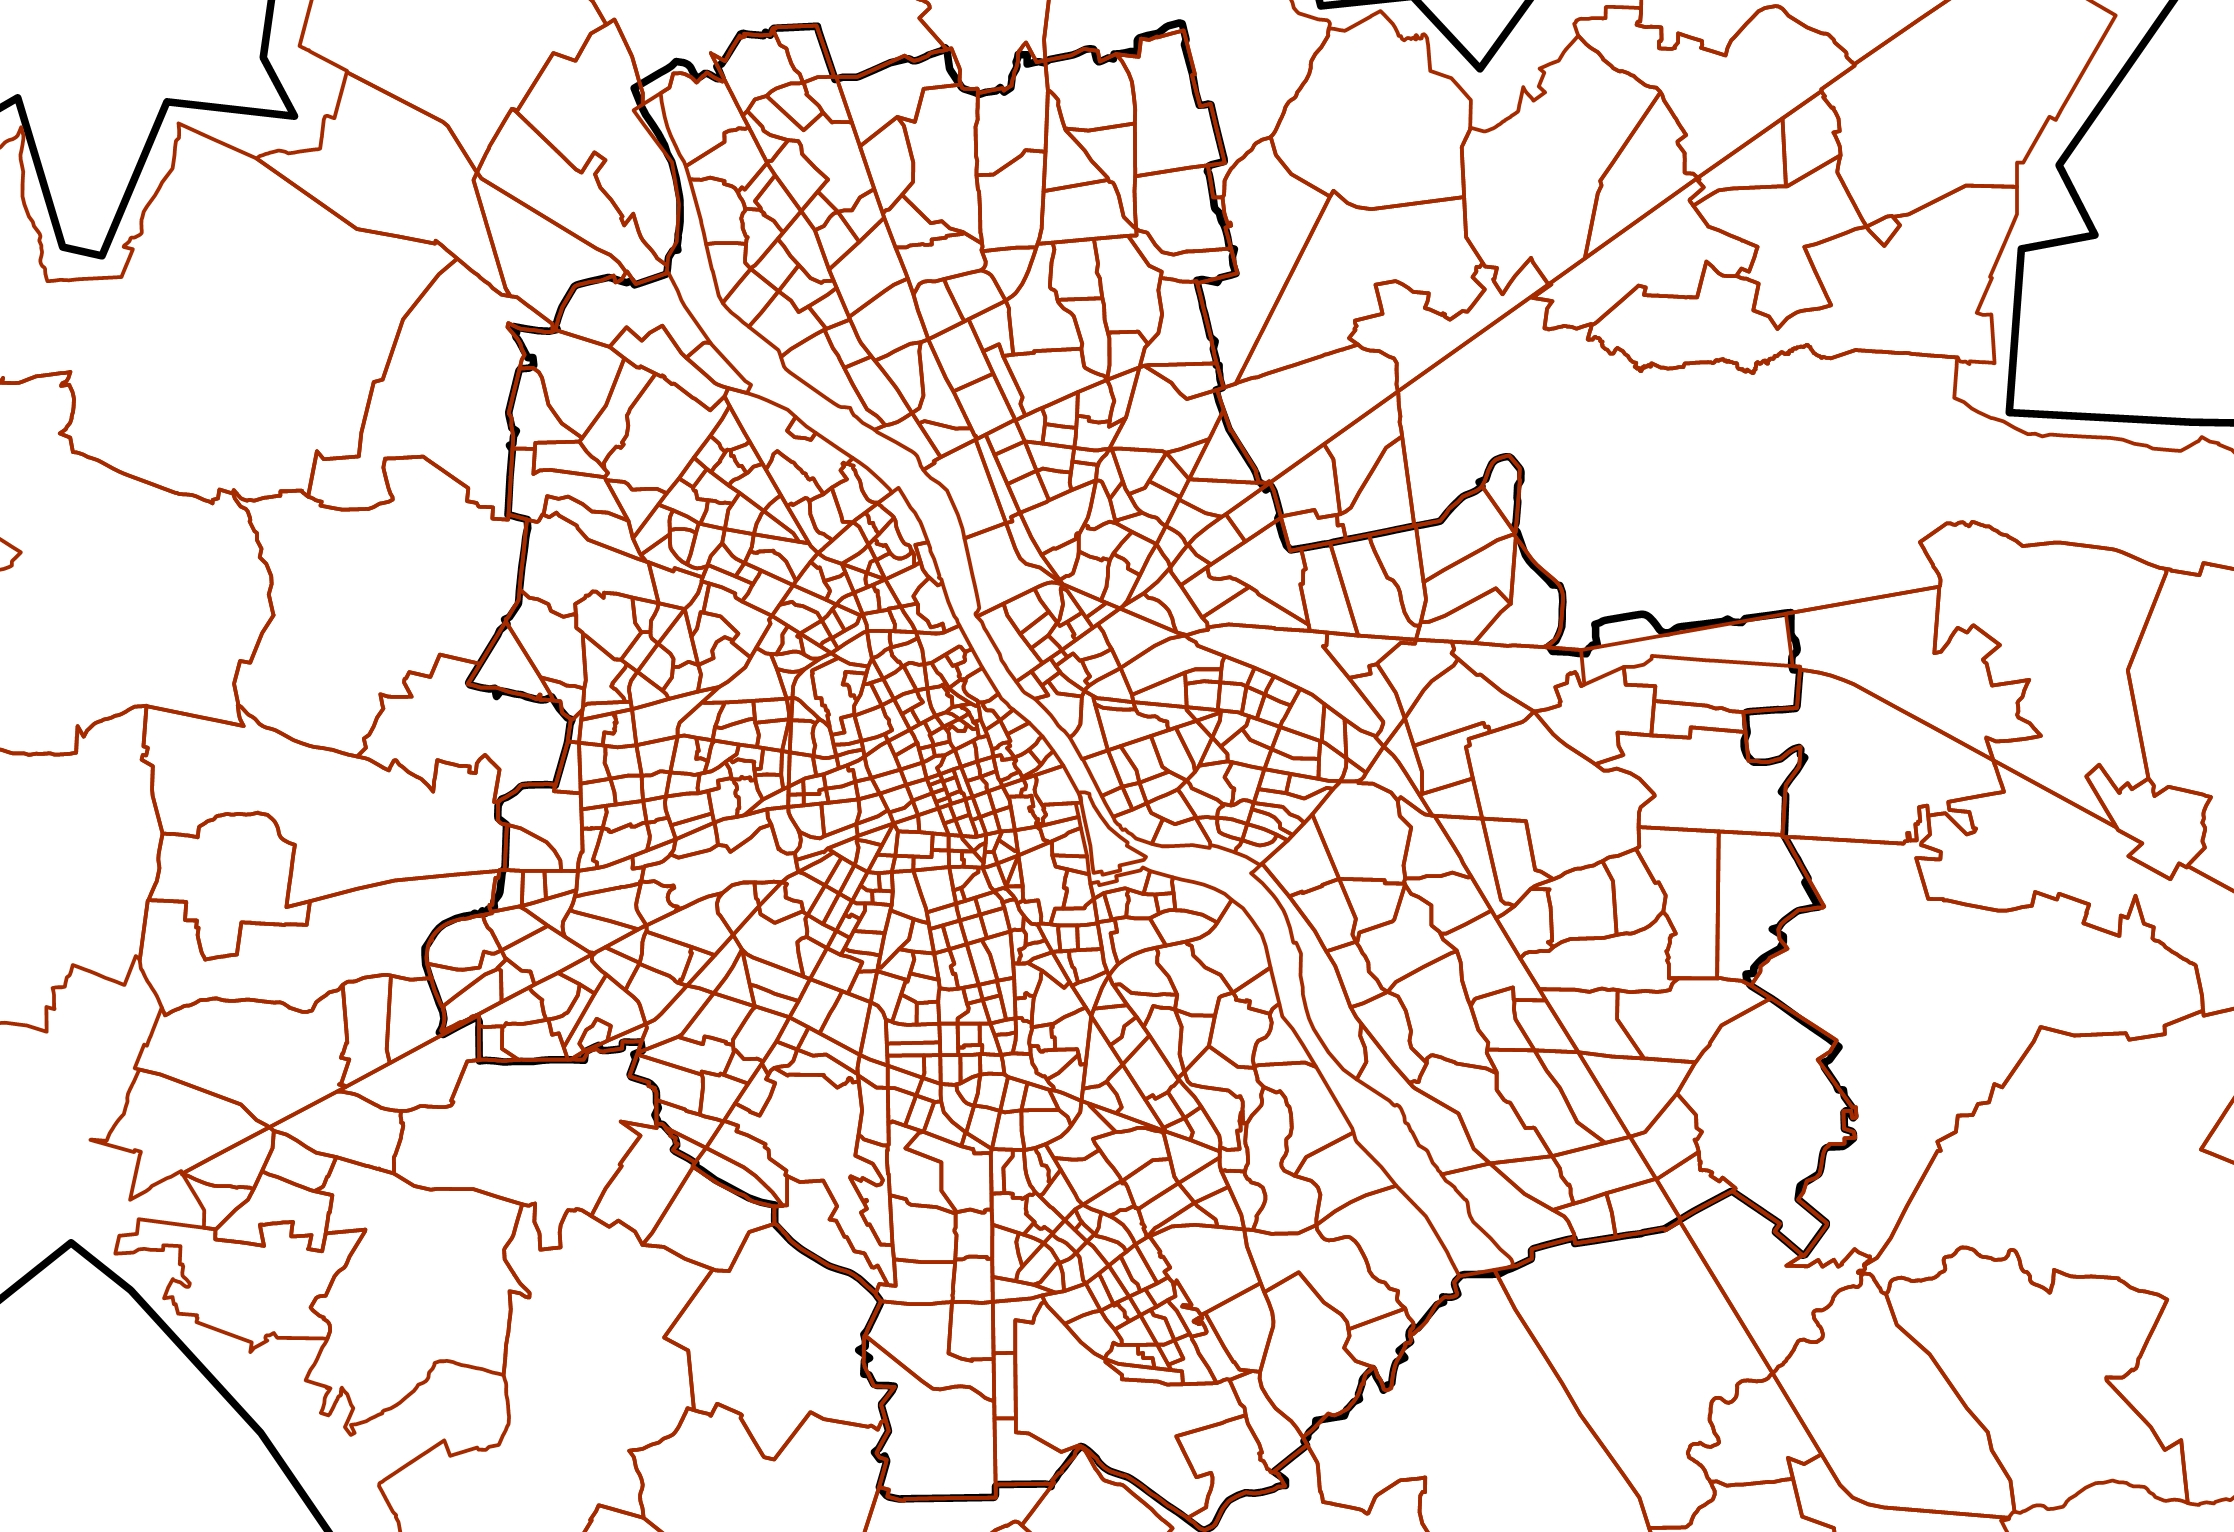
\includegraphics[width=0.9\textwidth]{zones2}
 \end{center}  \end{figure} 
\end{frame}

\begin{frame}{Rejony}
\begin{figure}\begin{center}
\includegraphics[width=0.9\textwidth]{zones3}
 \end{center}  \end{figure} 
\end{frame}

\subsection{Model popytu}
\begin{frame}{Motywacje}{ruch wewnętrzny}
\begin{figure}\begin{center}
\includegraphics[width=0.5\textwidth]{strata}
 \end{center}  \end{figure} 
\end{frame}

\subsection{Produkcja}
\begin{frame}{Produkcja}{Dom-Szkoła}
\begin{figure}\begin{center}
\includegraphics[width=0.9\textwidth]{prod_HE}
 \end{center}  \end{figure} 
\end{frame}

\begin{frame}{Produkcja}{Praca-Dom}
\begin{figure}\begin{center}
\includegraphics[width=0.9\textwidth]{prod_WH}
 \end{center}  \end{figure} 
\end{frame}

\begin{frame}{Produkcja}{Praca-Dom}
\begin{figure}\begin{center}
\includegraphics[width=0.9\textwidth]{prod_WH2}
 \end{center}  \end{figure} 
\end{frame}

\begin{frame}{Produkcja}{Potoki wyjazdowe - samochodowe}
\begin{figure}\begin{center}
\includegraphics[width=0.9\textwidth]{zone_bundle}
 \end{center}  \end{figure} 
\end{frame}

\begin{frame}{Produkcja}{Potoki wyjazdowe - pasażerskie}
\begin{figure}\begin{center}
\includegraphics[width=0.9\textwidth]{zone_bundle_PuT}
 \end{center}  \end{figure} 
\end{frame}

\section{Potoki w sieci}
\subsection{Komunikacja Zbiorowa}
\begin{frame}{Potoki pasażerów}
\begin{figure}\begin{center}
\includegraphics[width=0.9\textwidth]{put_flows1}
 \end{center}  \end{figure} 
\end{frame}

\begin{frame}{Potoki pasażerów}
\begin{figure}\begin{center}
\includegraphics[width=0.9\textwidth]{put_flows2}
 \end{center}  \end{figure} 
\end{frame}

\begin{frame}{Potoki pasażerów}
\begin{figure}\begin{center}
\includegraphics[width=0.9\textwidth]{put_flows3}
 \end{center}  \end{figure} 
\end{frame}

\begin{frame}{Potoki pasażerów}{wsiadający, wysiadający, przesiadający się na przystankach}
\begin{figure}\begin{center}
\includegraphics[width=0.9\textwidth]{stop_flows}
 \end{center}  \end{figure} 
\end{frame}


\subsection{Komunikacja Indywidualna}
\begin{frame}{Potoki pojazdów}
\begin{figure}\begin{center}
\includegraphics[width=0.9\textwidth]{prt_flows1}
 \end{center}  \end{figure} 
\end{frame}

\begin{frame}{Potoki pojazdów}
\begin{figure}\begin{center}
\includegraphics[width=0.9\textwidth]{prt_flows2}
 \end{center}  \end{figure} 
\end{frame}

\begin{frame}{Relacje skrętne}
\begin{figure}\begin{center}
\includegraphics[width=0.9\textwidth]{turn_flows}
 \end{center}  \end{figure} 
\end{frame}


\begin{frame}{Przepływ przez odcinek}{Wisłostrada}
\begin{figure}\begin{center}
\includegraphics[width=0.9\textwidth]{bundle_link}
 \end{center}  \end{figure} 
\end{frame}

\begin{frame}{Dziękuję za uwagę}
dr inż. Rafał Kucharski \\
Politechnika Krakowska
rkucharski _at_ pk.edu.pl
\end{frame}


\end{document}

